\documentclass[12pt,a4paper,twoside]{book}
\usepackage[utf8]{inputenc}
\usepackage{amsmath}
\usepackage{amstext}
\usepackage{amsfonts}
\usepackage{amssymb}
\usepackage{graphicx}
\usepackage{longtable}
\usepackage{booktabs}
\usepackage[bookmarks=true,colorlinks=true,urlcolor=blue,citecolor=blue,linkcolor=blue,unicode=true]{hyperref}
\usepackage[top=2.5cm, bottom=2.5cm]{geometry}
\usepackage{siunitx}

\setlength{\parindent}{0pt}
\setlength{\parskip}{6pt plus 2pt minus 1pt}
\setlength{\emergencystretch}{3em}  % prevent overfull lines
\providecommand{\tightlist}{%
  \setlength{\itemsep}{0pt}\setlength{\parskip}{0pt}}

%predefined commands
\newcommand{\Cb}{C_\beta} 
\newcommand{\eq}{\!=\!} 
\newcommand{\Gauss}{\mathcal{N}} 
\renewcommand{\H}{\mathbf{H}} 
\newcommand{\Hij}{\H_{ij}} 
\newcommand{\I}{\mathbf{I}} 
\newcommand{\Lijk}{\mathbf{\Lambda}_{ij,k}}
\newcommand{\Lk}{\mathbf{\Lambda}_k}
\newcommand{\LLreg}{L\!L_\mathrm{reg}}
\newcommand{\muijk}{\mathbf{\mu}_{ij,k}}
\newcommand{\muk}{\mathbf{\mu}_k}
\newcommand{\neff}{N_\mathrm{eff}}
\renewcommand{\r}{\mathbf{r}}
\newcommand{\rij}{r_{ij}}
\newcommand{\seq}{\mathbf{x}}
\newcommand{\Qij}{\mathbf{Q}_{ij}}
\newcommand{\q}{\mathbf{q}}
\newcommand{\qij}{\mathbf{q\prime}_{ij}}
\newcommand{\Sn}{\mathcal{S}_n}
\renewcommand{\v}{\mathbf{v}}
\newcommand{\vi}{\mathcal{v}_{i}}
\newcommand{\via}{\mathcal{v}_{ia}}
\newcommand{\w}{\mathbf{w}}
\newcommand{\wij}{\mathbf{w}_{ij}}
\newcommand{\wijab}{\mathcal{w}_{ijab}}
\newcommand{\wijcd}{\mathcal{w}_{ijcd}}
\newcommand{\wklcd}{\mathcal{w}_{klcd}}
\newcommand{\X}{\mathbf{X}}
\newcommand{\angstrom}{\si{\angstrom}}


% Numbering of sections unto depth=5
\setcounter{secnumdepth}{5}

% Table of contents formatting
\renewcommand{\contentsname}{Table of Contents}
\setcounter{tocdepth}{1}

% Headers and page numbering 
\usepackage{fancyhdr}
\pagestyle{plain}

% Chapter styling
\usepackage[grey]{quotchap}
\makeatletter 
\renewcommand*{\chapnumfont}{%
  \usefont{T1}{\@defaultcnfont}{b}{n}\fontsize{80}{100}\selectfont% Default: 100/130
  \color{chaptergrey}%
}
\makeatother


%------------------- Definition of LMU title pages
\newcommand{\LMUCover}[3]{
    \thispagestyle{empty}
    {\parindent0cm \rule{\linewidth}{.7ex}}
    
    \begin{flushright}
      \vspace*{\stretch{1}}
      \sffamily\bfseries\Huge
      #1\\
      \vspace*{\stretch{1}}
      \sffamily\bfseries\large
      #2
      \vspace*{\stretch{1}}
    \end{flushright}
  
    \rule{\linewidth}{.7ex}
    \vspace*{\stretch{5}}
    \vspace*{\stretch{1}}
    
    \begin{center}\sffamily\LARGE{#3}\end{center}
}



\newcommand{\LMUTitlePage}[4]{
    \thispagestyle{empty}
    \vspace*{\stretch{1}}
    
    \begin{center}
      \Large Dissertation zur Erlangung des Doktorgrades der Fakultät für Chemie und Pharmazie der Ludwig-Maximilians-Universität München
    \end{center}
    
    \vspace*{\stretch{1}}
    {\parindent0cm \rule{\linewidth}{.7ex}}
    
    \begin{flushright}
      \vspace*{\stretch{1}}
      \sffamily\bfseries\Huge
      #1\\
      \vspace*{\stretch{1}}
    \end{flushright}
  
    \rule{\linewidth}{.7ex}

    \vspace*{\stretch{3}}
    \begin{center}
      \Large vorgelegt von\\
      \Large #2\\
      \Large geboren in #3\\
      \vspace*{\stretch{2}}
      \Large München, den #4
    \end{center}
}


\newcommand{\LMUErklaerung}[5]{
    \thispagestyle{empty}
    \begin{flushleft}
      \large \textbf{Erklärung} \\[1mm]
      \large Diese Dissertation wurde im Sinne von §7 der Promotionsordnung vom 28. November 2011 von #2 betreut.
      \bigskip
  
      \large \textbf{Eidesstattliche Versicherung}\\[1mm]
      \large Diese Dissertation wurde eigenständig und ohne unerlaubte Hilfe erarbeitet.
      \vspace{5em}
  
      \dots\dots\dots   \dots\dots\dots \hfill \dots\dots\dots\dots\dots\dots\dots\dots\\
      \large Ort, Datum \hfill #1
      \vfill
  
  
      \large Dissertation eingereicht am: \hfill #4
      \bigskip
    
      \large Erstgutachter:  #2 \hfill \dots\dots\dots\dots\dots\dots\dots
      \bigskip
    
      \large Zweitgutachter: #3 \hfill \dots\dots\dots\dots\dots\dots\dots
      \bigskip
    
      \large Tag der mündlichen Prüfung: \hfill #5
    \end{flushleft}
}


\usepackage{amsthm}
\newtheorem{theorem}{Theorem}[chapter]
\newtheorem{lemma}{Lemma}[chapter]
\theoremstyle{definition}
\newtheorem{definition}{Definition}[chapter]
\newtheorem{corollary}{Corollary}[chapter]
\newtheorem{proposition}{Proposition}[chapter]
\theoremstyle{definition}
\newtheorem{example}{Example}[chapter]
\theoremstyle{remark}
\newtheorem*{remark}{Remark}
\begin{document}

\frontmatter

%%% LMU cover page
\LMUCover
	{Bayesian Model for Prediction of Protein Residue-Residue Contacts}
	{Susann Vorberg}
	{15.10.2017}

\newpage
\thispagestyle{empty}
\cleardoublepage

%%% LMU title page
\LMUTitlePage
	{Bayesian Model for Prediction of Protein Residue-Residue Contacts}
	{Susann Vorberg}
	{Leipzig, Germany}
	{15.10.2017}

\newpage
\thispagestyle{empty}
\cleardoublepage

%%% LMU statement page
\LMUErklaerung
	{Susann Vorberg}
	{Dr. Johannes Soeding}
	{Prof. Dr. Julien Gagneur}
	{15.10.2017}
	{15.12.2017}

\newpage
\thispagestyle{empty}
\cleardoublepage
\frontmatter\setcounter{page}{1}

\chapter*{Summary}\label{summary}
\addcontentsline{toc}{chapter}{Summary}

Awesome contact prediction project abstract

\chapter*{Acknowledgements}\label{acknowledgements}
\addcontentsline{toc}{chapter}{Acknowledgements}

I thank the world.

\tableofcontents
\addcontentsline{toc}{chapter}{Table of Contents}

\mainmatter \setcounter{page}{1}

\chapter{Introduction}\label{general-intro}

dsfgdsfg \(\AA\) ds dfg

In his Nobel Prize speech in 1973
{[}\protect\hyperlink{ref-Anfinsen1973}{1}{]} Anfinsen postulated one of
the basic principles in molecular biology, which is known as
\emph{Anfinsen's dogma}: a protein's native structure is uniquely
determined by its amino acid sequence. With certain exceptions (e.g.
\protect\hyperlink{abbrev}{IDP}
{[}\protect\hyperlink{ref-Wright1999}{2}{]}), this dogma has proven to
hold true for the majority of proteins.

Ever since, it is regarded as the biggest challenge in structural
bioinformatics {[}\protect\hyperlink{ref-Samish2015}{3}{]}, to realiably
predict a protein's structure given only its amino acid sequence.
\emph{De-novo} protein structure prediction methods use physical or
knowledge based energy potentials to find a protein conformation that
minimizes the protein's energy landscape. However, these methods are
limited by the complexity of the conformational space and the accuracy
of the energy potentials. Considering a protein with 150 amino acids,
that has approximately 450 degrees of freedom, Regarding the rotational
and translational degrees of freedom of the protein chain, the
complexity scales with XXX
{[}\protect\hyperlink{ref-Anfinsen1973}{1}{]}.

Far more successfull are template-based modelling approaches. Given the
observation that structure is more conserved than sequence in a protein
family {[}\protect\hyperlink{ref-Lesk1980}{4}{]}, the structure of a
target protein can be inferred from a homologue protein
{[}\protect\hyperlink{ref-Sander1991}{5}{]}. The degree of structural
conservation is linked to the level of pairwise sequence identity
{[}\protect\hyperlink{ref-Chothia1986}{6}{]}. Therefore, the accuracy of
a model crucially depends on the sequence identity between target and
template and determines the applicability of the model
{[}\protect\hyperlink{ref-Marti-Renom2000}{7}{]}. By definition,
homology derived models are unable to capture new folds
{[}\protect\hyperlink{ref-Dorn2014}{8}{]} and their main limitation lies
in the availability of suitable templates.

\begin{figure}
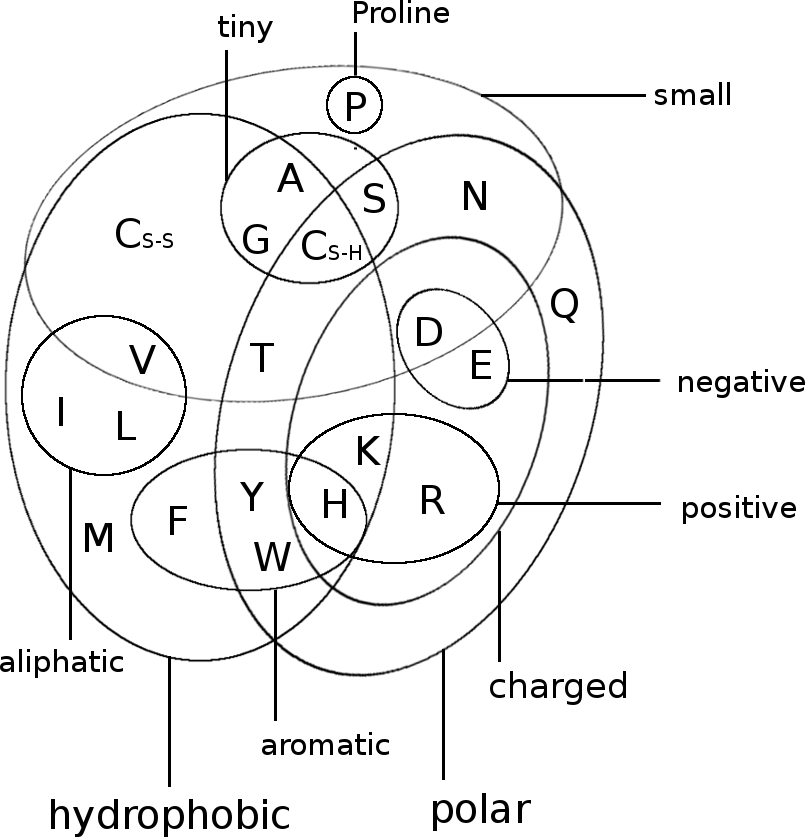
\includegraphics[width=1\linewidth]{img/amino_acid_physico_chemical_properties_venn_diagramm} \caption{Yearly growth of number of solved structures in the PDB[@Berman2000] and protein sequences in the Uniprot[@TheUniProtConsortium2013].}\label{fig:seq-str-gap}
\end{figure}

Unfortunately, the number of solved protein structures increases only
slowly, as experimental methods are both time consuming and expensive
{[}\protect\hyperlink{ref-Dorn2014}{8}{]}. The
\protect\hyperlink{abbrev}{PDB}{[}\protect\hyperlink{ref-Berman2000}{9}{]}
is the main repository for marcomolecular structures and currently (Jul
2017) holds about 120 000 atomic models of proteins. The primary
technique for determining protein structures is X-ray crystallography,
accounting for roughly 90\% of entries in the
\protect\hyperlink{abbrev}{PDB}. About 9\% of protein structures have
been solved using \protect\hyperlink{abbrev}{NMR} and less than 1\%
using \protect\hyperlink{abbrev}{EM} (see FIG 1).

All three experimental techniques have advantages and limitations with
respect to certain modelling aspects. X-ray crystallography requires the
protein to form crystals, which is an arduous and sometimes impossible
task. Furthermore, crystal packing forces the protein into a unnatural
and rigid environment preventing the observation of conformational
flexibility. NMR studies the protein in an physiological environment in
solution and enables the study of protein dynamics as ensembles of
protein structures can be observed. However, NMR is limited to look at
small proteins. Recently, EM has undergone a ``resolution revolution''
{[}\protect\hyperlink{ref-Egelman2016}{10}{]} and macromolecular
structures have been solved with resolutions up to 2A{[}citation{]}. The
limit of cryo-EM lies in the size of proteins.

Compared to the tedious task of revealing atomic resolution of a protein
tertiary structure, it has become very easy to decipher the primary
sequence of proteins. With the latest sequencing technologies
{[}examples{]}, it takes only hours to sequence millions of basepaires
at low costs {[}example numbers{]} and the number of sequenced genomes
has risen tremendously. The UniProtKB
{[}\protect\hyperlink{ref-TheUniProtConsortium2013}{11}{]}, the leading
resource for protein sequences, contains more than 80 million sequence
entries (24 July 2017).

Consequently, the gap between the number of protein structures and
sequences is still growing and even new developments as single protein
structure determination {[}{\textbf{???}}{]} are not expected to close
this gap near in time. {[}Figure sequence structure gap{]}

Protein structure determines protein function. Therefore, structural
insights are of uttermost importance. They are essential for a detailed
understanding of chemical reactions, regulatory processes and transport
mechanisms. They are fundamental for the design of drugs and
antibiotics. Moreover structural abnormalities can lead to misfolding
and aggregation potentially causing diseases so studying them is
pathologically relevant.

The aformentioned trends illustrate the need of computational methods
and motivate research to solve \emph{Ansinsens Dogma} to reliably
predict protein structures from sequence alone.

\section{Protein Structure}\label{protein-structure}

\begin{itemize}
\tightlist
\item
  Primary: Amino Acid Sewuence
\item
  Secondary: Helices, sheets, coils, repeats,..
\item
  tertiary: interaction of secondary structure elementws
\item
  quartary: interaction of domains
\end{itemize}

\subsection{Amino Acid Interactions}\label{amino-acid-interactions}

The Venn diagram in figure
\ref{fig:amino-acid-physico-chemical-properties} displays a typical
classification of amino acids with respect to their physico-chemical
properties.

The aromatic amino acids tryptophan (W), tyrosine (Y), phenylalanine
(F), and histidine (H) contain an aromatic ring system. Generally,
aromatic ring systems are planar, and electons are shared over the whole
ring structure. Interactions between aromatic residues have very
constrained geometries regarding the angle between the centroid of their
rings. The \(\pi\)-electron systems favour T-shaped or offset stacked
conformations {[}\protect\hyperlink{ref-Waters2002}{12}{]}. Preferred
distances between aromatic residues have been observed between
4.5\(\AA \; \;\) and 7\(\AA \; \;\) of their ring centroids
{[}\protect\hyperlink{ref-Burley1985}{13}{]}.

Cysteine (C) residues can form disulphide bonds, which are the only
covalent bonds between two amino acid side chains. They comprise the
strongest side chain interactions in protein structures and their length
varies between 3.5\(\AA \; \;\) to 4\(\AA \; \;\). Disulphide bonds also
have a well defined geometry: there are five dihedral angles in a
disulphide bond resulting in 20 different possible configurations. Only
one configuration is favoured so that the dihedral angle between the
carbon and sulfur atoms is close to 90 degrees
{[}\protect\hyperlink{ref-Thornton1981}{14}{]}. They play a very
important role in stabilizing protein structures. The number of
disulfide bonds is negatively correlated with protein length: smaller
proteins have more disulfide bonds helping to stabilize the structure in
absence of strong hydrophobic packing in the core. It has also been
found that disulfide bonds are more frequently observed in proteins of
hyperthermophilic bacteria, being positively selected for increased
stability {[}\protect\hyperlink{ref-Bastolla2005}{15}{]}.

Salt bridges are based on electrostatic interactions between positively
charged residues (arginine (R) and lysine (K)) and negatively charged
residues (aspartic acid (D) and glutamic acid (E)). The strength of
electrostatic interactions, as described by Coulomb's law, decreases
with distance between the point charges at the functional groups. It has
been found to be maximal at 4\(\AA \; \;\) with respect to the
functional groups of the both residues
{[}\protect\hyperlink{ref-Donald2011}{16}{]}.

Hydrogen bonds can be formed between a donor residue which possesses an
hydrogen atom attached to a strongly electronegative atom and an
acceptor residue which possesses an electronegative atom with a lone
electron pair. They are electrostatic interactions as well and thus
their strength depends on distance as well. Hydrogen bonds are formed at
distances of 2.4\(\AA \; \;\) to 3.5\(\AA \; \;\) between the
non-hydrogen atoms (Berg JM, Tymoczko JL, 2002).

Salt bridges as well as hydrogen bonds have strong geometric preferences
(Kumar and Nussinov, 1999). The geometry of a hydrogen bond depends on
the angle between the HB donor, the hydrogen atom and the HB acceptor
(Torshin et al., 2002).

Cation--\(\pi\) interactions are formed between positively charged or
partially charged amino acids with amino groups (K,R,Q,E) and aromatic
residues (W,Y,F,H). The preferential distance of the amino group to the
\(\pi\)-electron system has been determined between 3.4\(\AA \; \;\) and
6\(\AA \; \;\) {[}\protect\hyperlink{ref-Burley1986}{17}{]}
{[}\protect\hyperlink{ref-Crowley2005}{18}{]} Their role in stabilizing
protein structures is still under debate
{[}\protect\hyperlink{ref-Slutsky2004}{19}{]}.

Proline residues are conformationally restricted, with the alpha-amino
group of the backbone directly attached to the side chain. The sterical
rigidity of the proline side chain restricts the backbone angle and thus
affects secondary structure formation. Proline is known as a
helix-breaker. Whereas other aromatic side chains are defined by their
negatively charged \(\pi\) faces, the face of proline side chains is
partially positively charged. Thus, aromatic and proline residues can
interact favorably with each other. Once due to the hydrophobic nature
of the residues and also due to the interaction between the negatively
charged aroamtic \(\pi\) face and the polarized C-H bonds in proline,
called a CH/\(\pi\) interaction.

Petersen et al. (2012) found clear secondary structure elements
preferences for each amino acid pair. For example, residue pairs
containing Alanine and Leucine are predominantly found in buried
\(\alpha\)-helices, whereas pairs containing Isoleucine and Valine
preferentially are located in \(\beta\)-sheet environments. Of course,
solvent accessibility represents an important criterion for residue
interactions. Hydrophobic residues are rather buried in the structure,
whereas polar and charged residues are found more frequently on the
protein surface and interact with water molecules.

\begin{figure}
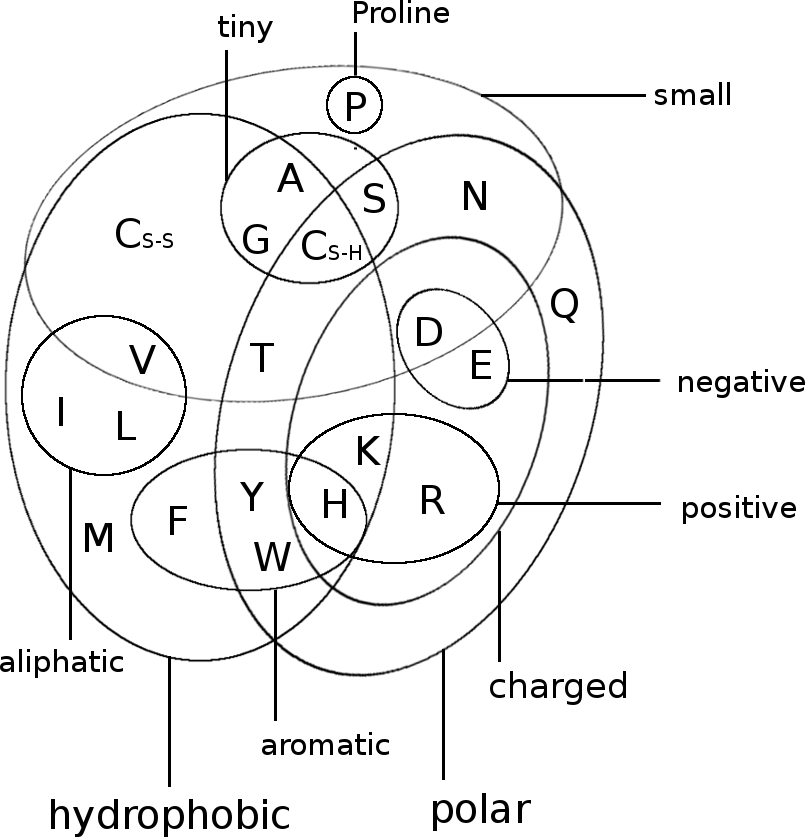
\includegraphics[width=0.5\linewidth]{img/amino_acid_physico_chemical_properties_venn_diagramm} \caption{Physico-chemical properties of amino acids. The 20 naturally occuring amino acids are grouped with respect to ten physico-chemical properties. Adapted from Figure 1a in [@Livingstone1993].}\label{fig:amino-acid-physico-chemical-properties}
\end{figure}

\section{Structure Prediction}\label{structure-prediction}

Despite the knowledge of Anfinsen's postulate, we are not able to
reliably predict the structure of a protein from its sequence alone.
Generally it is assumed that a protein folds into a unique, well-defined
native structure that is near the global free energy minimum
(fig:folding\_funnel). Levinthal's paradox
{[}\protect\hyperlink{ref-Levinthal1969}{20}{]} describes the complexity
of the folding process towards this minimum. It stresses the problem
that it is not possible for a protein to exhaustively search the
conformational space to get to its native fold. Due to the
``combinatorial explosion'' of possible conformations, an exhaustive
search would take unreasonably long. Hence, it is not a feasible
approach for structure prediction to scan all possible conformations.
Different approaches have been developed over time to overcome or elude
this problem.

\subsection{Template-based methods}\label{template-based-methods}

Homology modeling is by far the most successful approach to structure
prediction. The basic concept of this strategy relates to the fact that
structure is more conserved than sequence
{[}\protect\hyperlink{ref-Lesk1980}{4}{]}. After detecting a homologous
protein of known structure, that has sufficient sequence similarity, it
can be used as a template to model the structure of the target protein.

The degree of structural conservation is linked to the level of pariwise
sequence identity {[}\protect\hyperlink{ref-Chothia1986}{6}{]}. Homology
Modelling is assumed to yield reliably accurate models when query and
target protein share more than 30\(\%\) sequence similarity, depending
on the sequence length (\emph{safe homology zone})
{[}\protect\hyperlink{ref-Sander1991}{5}{]}. Below a threshold of
\textasciitilde{}20-35\% pairwise sequence identity
(\emph{twighlight-zone}) the number of false positives regarding
structural similarity explodes and structural inference becomes less
reliable and more than 95\% of structures are dissmilar
{[}\protect\hyperlink{ref-Rost1999}{21}{]}. Advances in remote homology
detection and alignment generation have improved the quality of models,
even beyond the once postulated limit of the \emph{twighlight-zone}
{[}\protect\hyperlink{ref-Yan2013}{22}{]}. Integration of multiple
templates has also proved to increase model quality
{[}\protect\hyperlink{ref-Meier2015}{23}{]}

After the identification of a suitable template, there are different
strategies that can be followed to obtain a model for the target
protein. The the backbone of the model is generated by simply copying
the coordinates of the target backbone atoms onto the model. Non-aligned
residues due to gaps in the alignment have to be modelled
\(\textit{de-novo}\), meaning from scratch. This can be done by a
knowledge-based search for suitable fragments in the PDB or by true
energy-based \(\textit{de-novo}\) modelling. When the backbone is
generated, the side chains are modelled, usually by searching rotamer
libraries for energetically favoured residue conformations. Finally, the
model is energetically optimized in an iterative procedure. Force fields
are applied to correct the backbone and side chain conformations
{[}\protect\hyperlink{ref-Gu2009}{24}{]}. Several automated pipelines
for homology modelling are well-established (Modeller
{[}\protect\hyperlink{ref-Eswar2007}{25}{]}, 3D-Jigsaw
{[}\protect\hyperlink{ref-Bates2001}{26}{]}, SwissModel
{[}\protect\hyperlink{ref-Arnold2006}{27}{]}) which allow more or less
manual intervention in the modelling process.

Fold Recognition describes the inverse folding problem {[}Bowie1993{]}:
instead of finding the compatible structure for a given sequence, one
tries to find sequences that fit onto a given structure. Whether the
query sequence fits a structure from the database is not determined by
sequence similarities but rather energetic or environment specific
measures. Thus, fold recognition methods are able to recognize
structural similarity even in the absence of sequence similarity. The
rationale basis for this strategy is the assumption that the fold space
is limited. It has been found that seemingly unrelated proteins often
adopt similar folds. This might be due to divergent evolution (proteins
are related, but homology cannot be detected at the corresponding
sequence level) or convergent evolution (functional requirements lead to
similar folds for unrelated proteins) {[}Gu2009{]}. Early approaches
include profile based methods. Here, the structural information of the
protein is encoded into profiles, which subsequently are aligned to the
sequences {[}Bowie1991,Fischer1996,Ouzounis1993{]}. Advanced techniques
are known as ``threading'' techniques, describing the process of
threading a sequence through a structure and determining the optimal fit
via energy functions. {[}Jones1992,Jones1998,Lemer1995{]}

\subsection{Template-free structure
prediction}\label{template-free-structure-prediction}

Ab initio or de-novo modeling techniques implement Anfinsen's Dogma most
closely in mimicking the folding process based only on physico-chemical
principles. Energy functions (physical or knowledge-based) are used to
describe the folding landscape and are minimized to arrive at the global
energy minimum corresponding to the native conformation. Since the
native conformation can be found near the global energy minimum of the
folding landscape, energy functions (physical or knowledge-based) have
been developed to describe this landscape. With respect to the idea of a
folding funnel, the energy function is minimized to mimic the folding
process that automatically leads to the global minimum. Again, there
exist numerous webservers that combine energy minimization, threading
techniques and fragment-based approaches, e.g.~Rosetta
{[}\textbackslash{}citep\{{]}Simons1999{]}, Tasser {[}Zhang2004,
Touchstone II Zhang2003{]}.

Drawbacks of these methods are the time requirements due to the
computational complexity of energy functions as well as their
inaccuracy.

Minimize a physical or knowledge-based energy function for the protein.
This has huge complexity due to large conformational space that needs to
be sampled.

\subsection{contact assisted de-novo
predictions}\label{contact-assisted-str-pred}

Structure Reconstruction from true contacts maps works well. Even a
small number of contacts is sufficient to reconstruct the fold of the
protein. Distance maps work even better.

What is the optimal distance cutoff to define a contact? Duarte et al
2010: between 8 and 12A Dyrka et al 2016 Konopka et al 2014 Sathyapriya
et al 2009

Many studies that successfuly predict structures denovo with the help of
predicted contact.

Vice versa, because contacts at large primary distances are rare, they
are most informative for protein structure prediction: Izarzugaza J,
Gran ˜a O, Tress M, Valencia A, Clarke N (2007) Assessment of
intramolecular contact predictions for CASP7

\section{Contact Prediction}\label{contact-prediction}

Contact Prediction refers to the prediction of physical contacts between
amino acid side chains in the 3D protein structure, given the protein
sequence as input.

Historically, contact prediction was motivated by the idea that
compensatory mutations between spatially neighboring residues can be
traced down from evolutionary records
{[}\protect\hyperlink{ref-Gobel1994}{28}{]}. As proteins evolve, they
are under selective pressure to maintain their function and
correspondingly their structure. Consequently, residues and interactions
between residues constraining the fold, protein complex formation or
other aspects of function are under selective pressure. Highly
constrained residues and interactions will be strongly conserved.
Another possibility to maintain structural integrity is the mutual
compensation of unbeneficial mutations. For example, the unfavourable
mutation of a small amino acid residue into a bulky residue in the
densely packed protein core might have been compensated in the course of
evolution by a particularly small side chain in a neighboring position.
Other physico-chemical quantities such as amino acid charge or hydrogen
bonding capacity can also be responsible for compensatory effects. In a
\protect\hyperlink{abbrev}{MSA}, sequences that descended from a common
ancestral sequence are aligned such that the homologous residues line up
with each other in columns. According to the hypothesis, compensatory
mutations show up as correlations between the amino acid types of pairs
of \protect\hyperlink{abbrev}{MSA} columns and can be used to infer
spatial proximity of residue pairs (see Figure
\ref{fig:correlated-mutations}).








\begin{figure}

{\centering 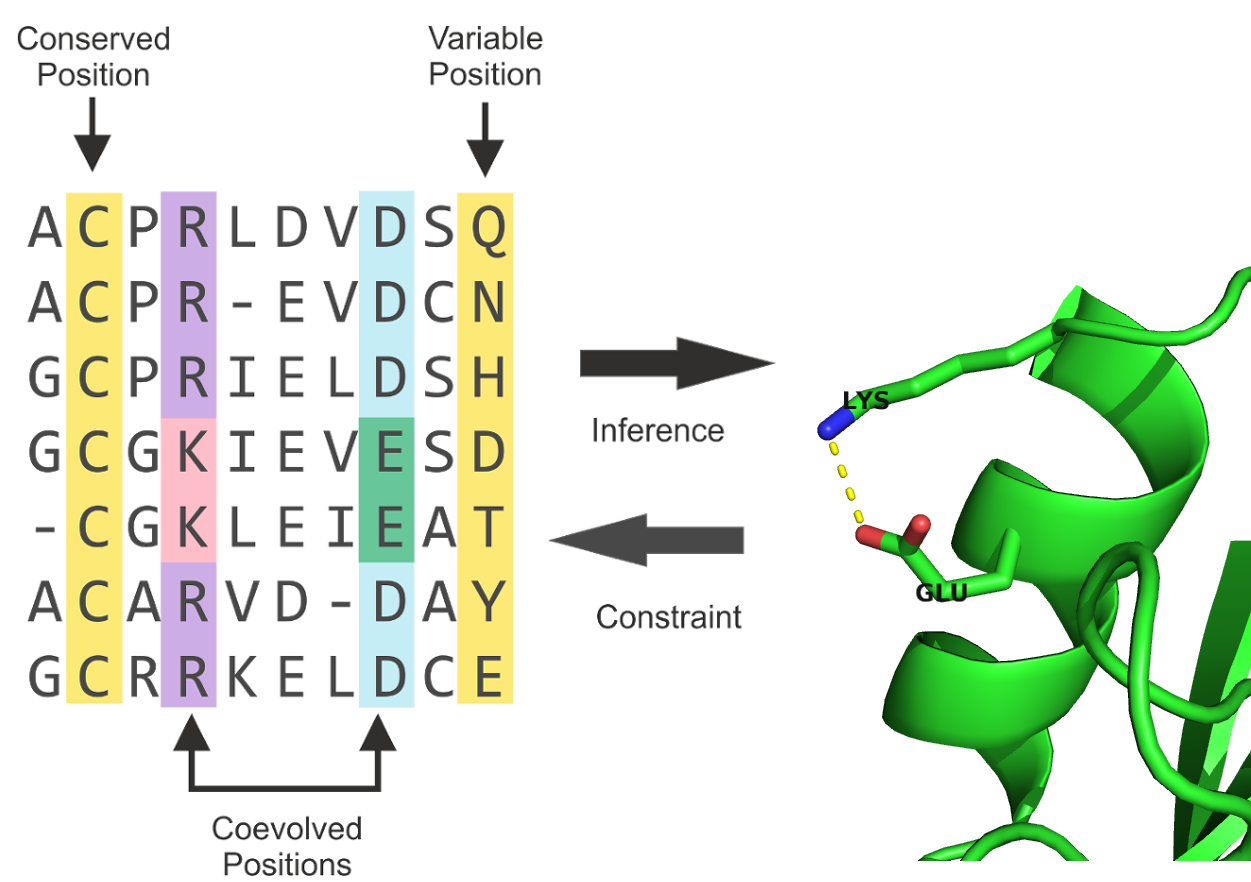
\includegraphics[width=0.8\linewidth]{img/intro/correlated-mutations-transparent} 

}

\caption{Compensatory mutations between
spatially neighboring residues subject to particular physico-chemical
constraints can leave coevolutionary record in protein sequences. Mining
protein family sequence alignments for residue pairs with strong
coevolutionary records using statistical models allows inference of
spatial proximity for these residue pairs.}\label{fig:correlated-mutations}
\end{figure}

Early methods from the 1990's were very inaccurate as the number of
available protein sequences was only small and weak statistical models
were prone to noise. It took until the end of the last decade that major
sources of noise could be eliminated and sophisticated statistical
models allowed for the distinction between transitively mediated and
causal interactions
{[}\protect\hyperlink{ref-Dunn2008}{29},\protect\hyperlink{ref-Weigt2009}{30}{]}.
With the steady increase in protein sequence data, purely machine
learning based methods emerged that are trained on features extracted
from \protect\hyperlink{abbrev}{MSAs}. Currently, the most accurate
methods to predict residue-residue contacts are meta-predictors,
combining one or several coevolution methods with sequence derived
features and other sources of information.

This chapter will give an overview over important previous methods, will
introduce the state-of-the-art statistical model for inferring
coevolutionary couplings and present well-known challenges for contact
prediction methods.

\subsection{Local Statistical Models}\label{local-methods}

Early contact prediction methods used local pairwise statistics to infer
contacts that regard pairs of amino acids in a sequence as statistically
independent from another. The drawback of these approaches is that they
do not account for transitive effects arising from chains of
correlations between multiple residue pairs as described in the section
on \protect\hyperlink{transitive-effects}{Transitive Effects}.

Several of these methods use correlation coefficient based measures,
such as Pearson correlation between amino acid counts, properties
associated with amino acids or mutational propensities at the sites of a
\protect\hyperlink{abbrev}{MSA}
{[}\protect\hyperlink{ref-Gobel1994}{28},\protect\hyperlink{ref-Neher1994}{31}--\protect\hyperlink{ref-Oliveira2002}{33}{]}.

Many methods have been developed that are rooted in information theory
and use \protect\hyperlink{abbrev}{MI} measures to describe the
dependencies between sites in the alignment
{[}\protect\hyperlink{ref-Clarke1995}{34}--\protect\hyperlink{ref-Martin2005}{36}{]}.
Phylogenetic and entropic biases have been identified as the major
sources of noise that confound the true coevolution signal
{[}\protect\hyperlink{ref-Martin2005}{36}--\protect\hyperlink{ref-Fodor2004}{38}{]}.
Different variants of \protect\hyperlink{abbrev}{MI} based approaches
try to address these effects and improve on the signal-to-noise ratio
{[}\protect\hyperlink{ref-Atchley2000}{37},\protect\hyperlink{ref-Tillier2003}{39},\protect\hyperlink{ref-Gouveia_Oliveira2007}{40}{]}.
The most prominent correction for background noises is
\protect\hyperlink{abbrev}{APC}, developed by Dunn et al. that
drastically removes background noise from entropic effects and is
discussed in section \ref{post-processing-heuristics}
{[}\protect\hyperlink{ref-Dunn2008}{29}{]}.

Another popular method is \emph{OMES} that essentially computes a
chi-squared statistic to detect the differences between observed and
expected pairwise amino acid frequencies for a pair of columns
{[}\protect\hyperlink{ref-Kass2002}{41},\protect\hyperlink{ref-Noivirt2005}{42}{]}.

Eventhough these methods cannot compete with modern predictors,
\emph{OMES} and \protect\hyperlink{abbrev}{MI} based scores often serve
as a baseline to benchmark the performance of new methods
{[}\protect\hyperlink{ref-DeJuan2013}{43},\protect\hyperlink{ref-Jones2012}{44}{]}.

\subsection{Global Statistical Models}\label{global-methods}

Global statistical models make predictions for a single residue pair
while considering all other pairs in the protein. By doing so they solve
the correlation versus causation phenomenon and distinguish direct from
indirect couplings which has been referred to in the literature as
\protect\hyperlink{abbrev}{DCA}
{[}\protect\hyperlink{ref-Weigt2009}{30},\protect\hyperlink{ref-Lapedes1999}{45}{]}.

In 1999 Lapedes et al. were the first to propose a global statistical
approach for the prediction of residue-residue contacts in order to
disentangle transitive effects
{[}\protect\hyperlink{ref-Lapedes1999}{45}{]}. They consider a Pott's
model that can be derived under a maximum entropy assumption and use the
model specific coupling parameters to infer interactions. At that time
the wider implications of this great advancement went unnoted but
meanwhile the Pott's Model has become the most prominent statistical
model for contact prediction. Section \ref{maxent} deals extensively
with the derivation and properties of the Pott's model, its application
to contact prediction and its numerous realizations.

A global statistical model not motivated by the maximum entropy approach
was proposed by Burger and Nijmwegen in 2010
{[}\protect\hyperlink{ref-Burger2008}{46},\protect\hyperlink{ref-Burger2010}{47}{]}.
Their fast Bayesian network model incorporates additional prior
information and phylogenetic correction via
\protect\hyperlink{abbrev}{APC} but cannot compete with the currently
most successfull pseudo-likelihood approaches presented in section
\ref{pseudo-likelihood}.

\subsection{Machine Learning Methods and
Meta-Predictors}\label{meta-predictors}

These methods combine abundant information on sequence and amino acid
properties in order to learn associations between input features and
residue-residue contacts. Methods differ mainly in the type of the
applied Machine Learning (ML) algorithm, e.g Neural Networks (NNs),
Support Vector Machines (SVMs) or Random Forests (RFs) and the chosen
input features, e.g.~contact predictions, solvent accessibility,
physico-chemical properties of amino acids, secondary structure
predictions or evolutionary information. (Kukic et al., 2014; Alfonso
Marquez-Chamorro, 2013; Li et al., 2011) The problem with these methods
is interpretability, as it is diffcult to elucidate which feature
patterns contribute in which amount to the model.

\begin{itemize}
\tightlist
\item
  combining different approaches
\item
  jones et al: overlap between methods but also many unique predictions
\item
  machine learning methods incorporate sequence-derived features:
\item
  secondary structure predictions
\item
  solvent accessibilty
\item
  contact potentials
\item
  msa properties
\item
  pssms
\item
  physico-chemcial properties of amino acids
\end{itemize}

However, Meta-predictors will improve if basic methods improve.
Ultra-deep learning paper identifies coevolution features as crucial
feature.

\subsection{Evaluating Contact Prediction
Methods}\label{intro-cp-evaluation}

Choosing an appropriate benchmark for contact prediction methods depends
on the further utilization of the predictions. Most prominently,
predicted contacts are used to assist structure prediction as outlined
in section \ref{contact-assisted-str-pred}. Therefore, one could in fact
assess the quality of structural models computed with the help of
predicted contacts. However, predicting structural models adds not only
another layer of computational complexity but also raises questions
about implementation details of the folding protocol. Generally it has
been found that a small number of accurate contacts is sufficient to
constrain the overal protein fold as discussed in section
\ref{contact-assisted-str-pred}.

From these considerations emerged a standard benchmark that evaluates
the mean precision over a testset of proteins with known high quality 3D
structures with respect to the top scoring predictions from every
protein. The number of top scoring predictions per protein is typically
normalized with respect to protein length \(L\) and precision is defined
as the number of true contacts among the top scoring predicted contacts.
Usually, a pair of residues is defined to be in contact when the
distance between their \(\Cb\) atoms (\(C\alpha\) in case of glycine) is
less than 8\(\AA\) in the reference protein structure
{[}\protect\hyperlink{ref-Monastyrskyy2015}{48}{]}.

\textbf{Sequence Separation}

Local residue pairs separated by only some positions in sequence (e.g
\(|i-j| < 6\)) are usually filtered out for evaluation of contact
prediction methods. They are trivial to predict as they typically
correspond to contacts within secondary structure elements and reflect
the local geometrical constraints. Figure \ref{fig:Cb-distribution}
shows the distribution of \(\Cb\) distances for various minimal sequence
separation thresholds.






\begin{figure}
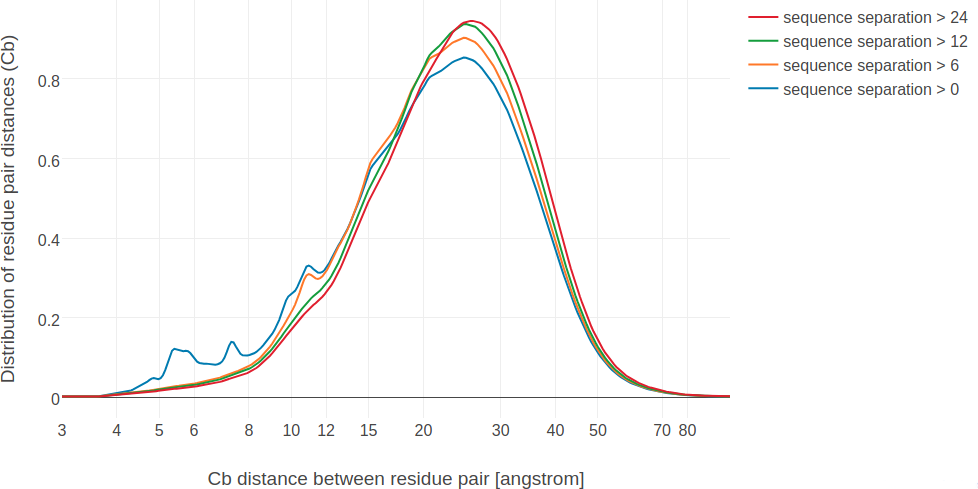
\includegraphics[width=1\linewidth]{img/dataset_statistics/Cb_distribution_all_data43579541_log} \caption{Distribution of residue pair \(\Cb\)
distances over \textasciitilde{}6000 proteins in the dataset (see
Methods \ref{dataset}) at different minimal sequence separation
thresholds.}\label{fig:Cb-distribution}
\end{figure}

Without filtering local residue pairs (sequence separation 1), there are
several additional peaks in the distribution around \(5.5\AA \; \;\),
\(7.4\AA \; \;\) and \(10.6\AA \; \;\) that can be attributed to local
interactions in e.g.~helices (see Figure
\ref{fig:peaks-Cb-distribution}).









\begin{figure}
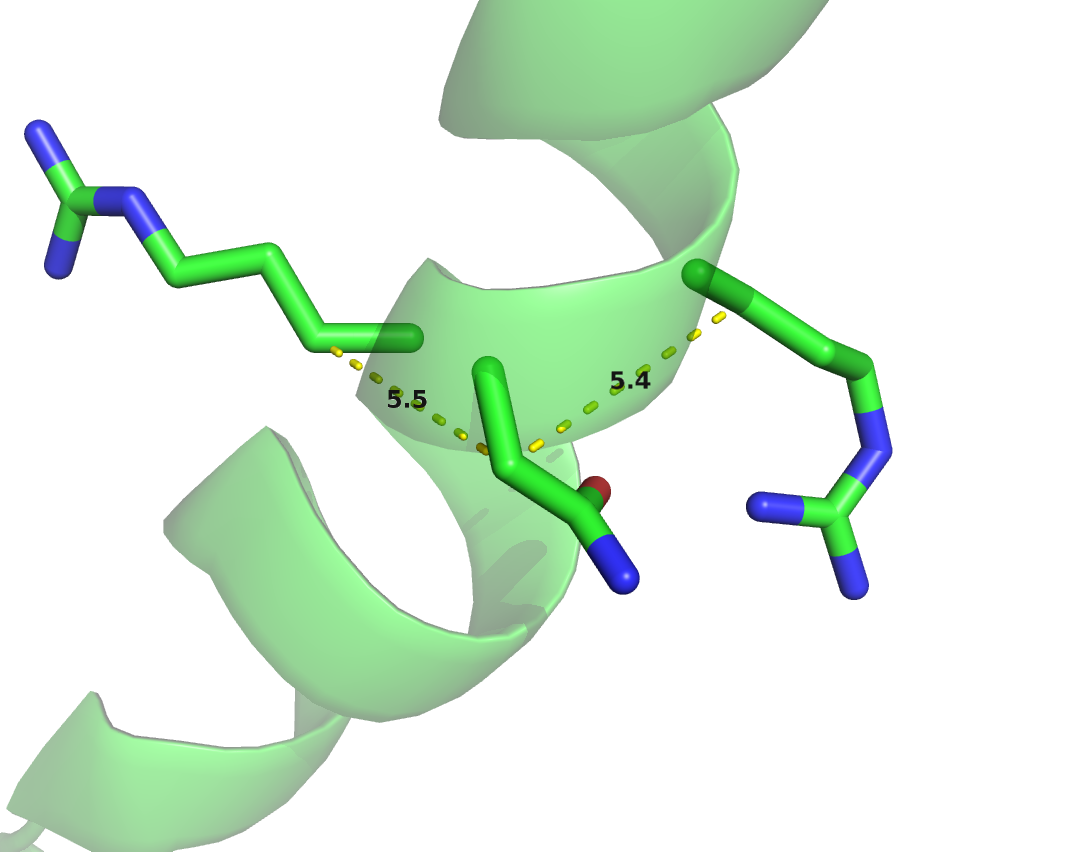
\includegraphics[width=0.5\linewidth]{img/dataset_statistics/cb_distribution_peak_5-6} 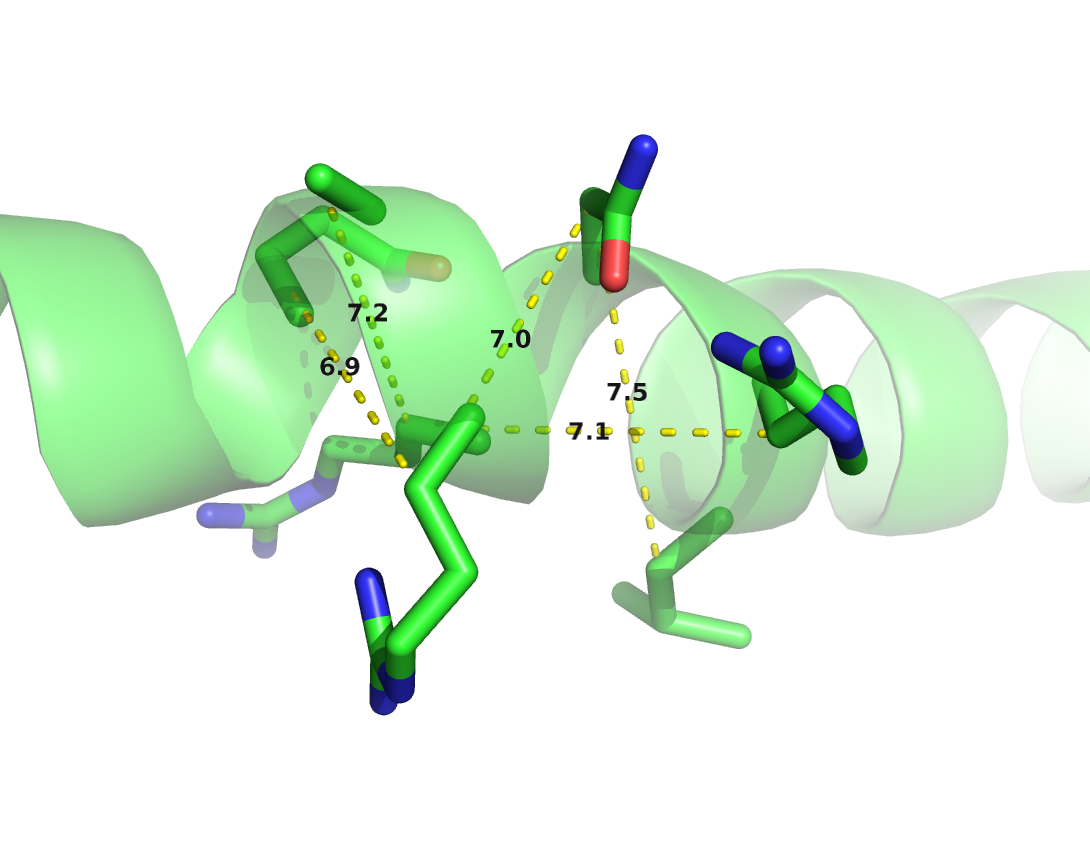
\includegraphics[width=0.5\linewidth]{img/dataset_statistics/cb_distribution_peak_7} \caption{\(\Cb\) distances between
neighboring residues in \(\alpha\)-helices. Left: Direct neighbors in
\(\alpha\)-helices have \(\Cb\) distances around \(5.4\AA \; \;\) due to
the geometrical constraints from \(\alpha\)-helical architecture. Right:
Residues separated by two positions (\(|i-j| = 2\)) are less
geometrically restricted to \(\Cb\) distances between \(7\AA \; \;\) and
\(7.5\AA \; \;\).}\label{fig:peaks-Cb-distribution}
\end{figure}

Commonly, sequence separation bins are applied to distuinguish short
(\(6 < |i-j| \le 12\)), medium (\(12 < |i-j| \le 24\)) and long range
(\(|i-j| > 24\)) contacts
{[}\protect\hyperlink{ref-Monastyrskyy2015}{48}{]}. Especially long
range contacts are of importance for structure prediction as they are
informative and able to constrain the overal fold of a protein
{[}{\textbf{???}}{]}.

\textbf{CASP}

CASP, the well-respected and independent competition for the structural
bioinformatic's community that is taking place every two years,
introduced the contact prediction category in 1996 and developed a
standard procedure for the assessment of predictions. The precision of
predicted long range (\(|i-j| > 24\)) contacts is assessed based on a
\(8 \AA \; \; \Cb\) distance threshold for proteins with no (or only
hard to detect) structural homologs. During CASP11 further evaluation
metrics have been introduced, such as Matthews correlation coefficient
and area under the precision-recall curve.

Currently best methods perform in the range XXX

\subsection{Maximum Entropy Modelling of Protein Families}\label{maxent}

The principle of maximum entropy, proposed by Jaynes in 1957
{[}\protect\hyperlink{ref-Jaynes1957a}{49},\protect\hyperlink{ref-Jaynes1957b}{50}{]},
states that the probability distribution which makes minimal assumptions
and best represents observed data is the one that is in agreement with
measured constraints (prior information) and has the largest entropy. In
other words, from all the distributions that are consistent with the
given data one chooses the distribution with maximal Shannon entropy.

Applied to the problem of modelling protein families, one seeks a
probability distribution \(p(\seq)\) for protein sequences
\(\seq = (x_1, \ldots, x_L)\) of length \(L\) from the protein family
under study. The categorical variables \(x_{i}\) can take one of
\(q=21\) values representing the 20 naturally occuring amino acids and a
gap (`-'). Given \(N\) sequences of the protein family in a
\protect\hyperlink{abbrev}{MSA} with
\(\X = \{ \seq_1, \ldots, \seq_N \}\), the empirically observed single
and pairwise amino acid frequencies can be calculated as

\begin{equation}
    \mathcal{f}_i(a) = \mathcal{f}(x_i\eq a) = \frac{1}{N}\sum_{n=1}^N I(x_{ni} \eq a) \\
    \mathcal{f}_{ij}(a,b) = \mathcal{f}(x_i\eq a, x_j\eq b) = \frac{1}{N} \sum_{n=1}^N I(x_{ni} \eq a, x_{nj} \eq b) \; .
 \label{eq:emp-freq}
\end{equation}

According to the maximum entropy principle, the distribution \(p(\seq)\)
should have maximal entropy and reproduce the empirically observed amino
acid frequencies, so that

\begin{align}
   \mathcal{f}(x_i\eq a)            &\equiv p(x_i\eq a)  \\
                                    &= \sum_{\seq\prime_1, \ldots, \seq\prime_L = 1}^{q} p(x\prime) I(x\prime_i \eq a) \\
  \mathcal{f}(x_i\eq a, x_j\eq b)   &\equiv p(x_i\eq a, x_j \eq b) \\
                                    &= \sum_{\seq\prime_1, \ldots, \seq\prime_L = 1}^{q}  p(x\prime) I(x\prime_i\eq a, x\prime_j \eq b)  \; .
 \label{eq:maxent-reproducing-emp-freq}
\end{align}

Solving for the distribution \(p(\seq)\) that maximizes the Shannon
entropy \(S= -\sum_{\seq\prime} p(\seq\prime) \log p(\seq\prime)\) while
satisfying the constraints given in eq.
\eqref{eq:maxent-reproducing-emp-freq} by introducing the Lagrange
multipliers \(\wij\) and \(\vi\),

\begin{align}
F \left[ p(\seq) \right] =& -\sum_{\seq\prime} p(\seq\prime) \log p(\seq\prime) \\
        & + \sum_{i=1}^L \sum_{a=1}^{q} \vi(a) \left( p(x_i\eq a) - \mathcal{f}(x_i\eq a) \right) \\
        & + \sum_{1 \leq i < j \leq L}^L \; \sum_{a,b=1}^{q} \wij(a,b) \left( p(x_i\eq a, x_j \eq b) - \mathcal{f}(x_i\eq a, x_j\eq b) \right) \\
        & + \Omega \left( 1-\sum_{\seq\prime} p(\seq\prime)  \right)
\label{eq:derivation-max-ent-model}
\end{align}

results in the formulation of an exponential model known as \emph{Potts
model} in statistical physics or \protect\hyperlink{abbrev}{MRF} in
statistics,

\begin{equation}
    p(\seq | \v, \w ) = \frac{1}{Z} \exp \left( \sum_{i=1}^L v_i(x_i) \sum_{1 \leq i < j \leq L}^L w_{ij}(x_i, x_j) \right) \; .
\label{eq:max-ent-model}
\end{equation}

The Lagrange multipliers \(\wij\) and \(\vi\) remain as model parameters
to be fitted to data. \(Z\) is a normalization constant also known as
\emph{partition function} that ensures the total probabilty adds up to
one by summing over all possible assignments to \(\seq\),

\begin{equation}
  Z = \sum_{\seq\prime_1, \ldots, \seq\prime_L = 1}^{q} \exp  \left( \sum_{i=1}^L v_i(x_i) \sum_{1 \leq i < j \leq L}^L w_{ij}(x_i, x_j) \right) \; .
  \label{eq:partition-fct-likelihood}
\end{equation}

\subsubsection{Model Properties}\label{model-properties}

The Potts model is specified by singlet terms \(\via\) which describe
the tendency for each amino acid a to appear at position \(i\), and pair
terms \(\wijab\), also called couplings, which describe the tendency of
amino acid a at position \(i\) to co-occur with amino acid b at position
\(j\). In contrast to mere correlations, the couplings explain the
causative dependence structure between positions by jointly modelling
the distribution of all positions in a protein sequence and thus account
for transitive effects (see \ref{local-methods}).

Maximum entropy models naturally give rise to exponential family
distributions that express useful properties for statistical modelling,
such as the convexity of the likelihood function which consequently has
a unique, global minimum
{[}\protect\hyperlink{ref-Wainwright2007}{51},\protect\hyperlink{ref-Murphy2012}{52}{]}.

The Potts model is a discrete instance of what is referred to as a
pairwise \protect\hyperlink{abbrev}{Markov random field} in the
statistics community. \protect\hyperlink{abbrev}{MRFs} belong to the
class of undirected graphical models, that represent the probability
distribution in terms of a graph with nodes and edges characterizing the
variables and the dependence structure between variables, respectively.

\hypertarget{gauge-invariance}{\paragraph{Gauge
Invariance}\label{gauge-invariance}}
\addcontentsline{toc}{paragraph}{Gauge Invariance}

As \(x_{ni}\) can take \(q=21\) values, the model has
\(L \! \times \! q + L(L-1)/2 \! \times \! q^2\) parameters but the
parameters are not uniquely determined as multiple parametrizations
yield identical probability distributions.

For example, adding a constant \(c_i\) to all elements in \(v_i\) for
any fixed position \(i\) or similarly adding a constant \(c_{ia}\) to
\(\via\) for any fixed position \(i\) and amino acid \(a\) and
subtracting the same constant from the \(qL\) coefficients \(\wijab\)
with \(b \in \{1, \ldots, q\}\) and \(j \in \{1, \ldots, L \}\) leaves
the probabilities for all sequences under the model unchanged, since
such a change will be compensated by a change of \(Z\) in eq.
\eqref{eq:partition-fct-likelihood}.

The overparametrization, referred to as \emph{gauge invariance} in
statistical physics literature, can be eliminated by removing
parameters. An appropriate choice of which parameters to remove,
referred to as \emph{gauge choice}, reduces the number of parameters to
\(L \! \times \! (q-1) + L(L-1)/2 \! \times \! (q-1)^2\). Popular gauge
choices are the \emph{zero-sum gauge} or \emph{Ising-gauge} used by
{[}\protect\hyperlink{ref-Weigt2009}{30}{]} imposed by the restraints,

\begin{equation}
    \sum_{a=1}^{q} v_{ia} = \sum_{a=1}^{q} \wijab = \sum_{a=1}^{q} w_{ijba} = 0
\label{eq:zero-sum-gauge}
\end{equation}

for all \(i,j,b\) or the \emph{lattice-gas gauge} used by
{[}\protect\hyperlink{ref-Morcos2011}{53},\protect\hyperlink{ref-Marks2011}{54}{]}
imposed by restraints

\begin{equation}
    \wij(q,a) = \wij(a,q) = \vi(q) = 0
\label{eq:ising-gauge}
\end{equation}

for all \(i,j,a\) {[}\protect\hyperlink{ref-Cocco2017}{55}{]}.

Alternatively, the indeterminacy can be fixed by including a
regularization prior (see next section). The regularizer selects for a
unique solution among all parametrizations of the optimal distribution
and therefore eliminates the need to choose a gauge
{[}\protect\hyperlink{ref-Koller2009}{56}--\protect\hyperlink{ref-Stein2015a}{58}{]}.

\paragraph{Regularization}\label{regularization}
\addcontentsline{toc}{paragraph}{Regularization}

The number of parameters in a Potts model is typically larger than the
number of observations, i.e.~the number of sequences in the
\protect\hyperlink{abbrev}{MSA}. Considering a protein of length
\(L=100\), there are approximately \(2 \times 10^6\) parameters in the
model whereas the largest protein families comprise only around \(10^5\)
sequences (see Figure \ref{fig:pfam}). An underdetermined problem like
this renders the use of regularizer neccessary in order to prevent
overfitting.

Typically, an L2-regularization is used that pushes the single and
pairwise terms smoothly towards zero and is equivalent to the logarithm
of a zero-centered Gaussian prior,

\begin{align}
  R(\v, \w)  &= \log \left[ \mathcal{N}(\v | \mathbf{0}, \lambda_v^{-1} I) \mathcal{N}(\w | \mathbf{0}, \lambda_w^{-1} I) \right] \\
             &= -\frac{\lambda_v}{2} ||\v||_2^2 - \frac{\lambda_w}{2} ||\w||_2^2 + \text{const.} \; ,
\label{eq:l2-reg}
\end{align}

where the strength of regularization is tuned via the regularization
coefficients \(\lambda_v\) and \(\lambda_w\)
{[}\protect\hyperlink{ref-Seemayer2014}{59}--\protect\hyperlink{ref-Kamisetty2013}{61}{]}.

\subsubsection{Intractability of the Partition
Function}\label{partition-function}

Typically, one obtains parameter estimates by maximizing the
log-likelihood function of the parameters over observed data. For the
Potts model, the log-likelihood function is computed over sequences in
the alignment \(\mathbf{X}\):

\begin{align}
    \text{LL}(\v, \w | \mathbf{X}) =& \sum_{n=1}^N \log p(\seq_n) \\
    =& \sum_{n=1}^N \left[ \sum_{i=1}^L v_i(x_{ni}) + \sum_{1 \leq i < j \leq L}^L w_{ij}(x_{xn}, x_{nj}) - \log Z \right] \\
\label{eq:full-log-likelihood}
\end{align}

However, optimizing the log-likelihood requires computing the partition
function \(Z\) given in eq. \eqref{eq:partition-fct-likelihood} that sums
\(q^L\) terms, with \(L\) being in the hundreds for naturally occurig
protein domains. Because of this exponential complexity in protein
length \(L\), it is computationally intractable to evaluate the
log-likelihood function at every iteration of an optimization procedure.

Several approximate solutions have been developed to sidestep the
infeasible computation of the partition function for the specific
problem of predicting contacts between residues that are briefly
explained in the next section.

\subsubsection{Solving the Inverse Potts
Problem}\label{solving-the-inverse-potts-problem}

In 1999 Lapedes et al. were the first to propose maximum entropy models
for the prediction of residue-residue contacts in order to disentangle
transitive effects {[}\protect\hyperlink{ref-Lapedes1999}{45}{]}. They
used an iterative Monte Carlo procedure to obtain estimates of the
partition function. As the calculations involved were very
time-consuming and at that time required supercomputing resources, the
wider implications were not noted yet.

In 2009 Weight et al proposed an iterative message-passing algorithm,
here referred to as \emph{mpDCA}, to approximate the partition function
{[}\protect\hyperlink{ref-Weigt2009}{30}{]}. Eventhough their approach
is computationally very expensive and in practive only applicable to
small proteins, they obtained remarkable results for the two-component
signaling system in bacteria.

Balakrishnan et al {[}\protect\hyperlink{ref-Balakrishnan2011}{62}{]}
were the first to apply pseudo-likelihood approximations to the full
likelihood in 2011. The pseudo-likelihood optimizes a different
objective and replaces the global partition function \(Z\) with local
estimates. Balakrishnan and colleagues applied their method
\emph{GREMLIN} to learn sparse graphical models for 71 protein families.
In a follow-up study in 2013
{[}\protect\hyperlink{ref-Kamisetty2013}{61}{]}, an improved version of
\emph{GREMLIN} incorporating prior information was evaluated in a
comprehensive benchmark tailored towards the contact prediction problem.

Also in 2011, Morcos et al. introduced a naive mean-field inversion
approximation to the partition function, named \emph{mfDCA}
{[}\protect\hyperlink{ref-Morcos2011}{53}{]}. This method allows for
drastically shorter running times as the mean-field approach boils down
to inverting the empirical covariance matrix calculated from observed
amino acid frequencies for each residue pair \(i\) and \(j\) of the
alignment. This study performed the first high-throughput analysis of
intradomain contacts for 131 protein families and facilitated the
prediction of protein structures from accurately predicted contacts in
{[}\protect\hyperlink{ref-Marks2011}{54}{]}.

The initial work by Balakrishnan and collegueas went almost unnoted as
it was not primarily targeted to the problem of contact prediction.
Ekeberg and collegueas independently developed the pseudo-likelihood
method \emph{plmDCA} and showed its superior precision towards
\emph{mfDCA} {[}\protect\hyperlink{ref-Ekeberg2013}{57}{]}.

A related approach to mean-field approximation is sparse inverse
covariance estimation, named \emph{PSICOV}, by Jones et al
{[}\protect\hyperlink{ref-Jones2012}{44}{]}. They use L1-regularization,
known as graphical Lasso, to invert the correlation matrix and learn a
sparse graphical model {[}\protect\hyperlink{ref-Friedman2008}{63}{]}.
Both procedures, \emph{mfDCA} and \emph{PSICOV}, assume the model
distribution to be a multivariate Gaussian. It has been shown by
Banerjee et al. (2008) that this dual optimization solution also applies
to binary data (as is the case in this application). In order to
represent the \protect\hyperlink{abbrev}{MSA} as continuous distributed,
each position is encoded as a 20-dimensional binary vector.

Another related approach to \emph{mfDCA} and \emph{PSICOV} is
\emph{gaussianDCA}, proposed in 2014 by Baldassi et al.
{[}\protect\hyperlink{ref-Baldassi2014}{64}{]}. Similar to the other
both approaches, they model the data as multivariate Gaussian but within
a simple Bayesian formalism by using a suitable prior and estimating
parameters over the posterior distribution.

So far, pseudo-likelihood maximization has proven to be the most
accurate approach with respect to the standard evaluation procedures for
contact prediction presented in the following section. Currently, there
exist several implementations of pseudo-likelihood maximization that
vary in slight details, perform similarly and thus are equally popular
in the community, such as CCMpred
{[}\protect\hyperlink{ref-Seemayer2014}{59}{]},
plmDCA{[}\protect\hyperlink{ref-Ekeberg2014}{60}{]} and GREMLIN
{[}\protect\hyperlink{ref-Kamisetty2013}{61}{]}.

\subsubsection{Pseudo-Likelihood}\label{pseudo-likelihood}

Instead of the full likelihood, Besag suggested to optimize a different
objective function that he called \emph{pseudo-likelihood}
{[}\protect\hyperlink{ref-Besag1975}{65}{]}. The pseudo-likelihood
approximates the joint probability with the product over conditionals
for each variable, i.e.~the conditional probability of observing one
variable given all the others:

\begin{equation}
  p(\seq | \v,\w) \approx   \prod_{i=1}^L p(x_i | \seq_{\backslash xi}, \v,\w) =  \prod_{i=1}^L \frac{1}{Z_i} \exp \left(  v_i(x_i) \sum_{1 \leq i < j \leq L}^L w_{ij}(x_i, x_j) \right)
\end{equation}

Here, the normalization term \(Z_i\) sums only over all assignments to
one position \(i\) in sequence:

\begin{equation}
  Z_i = \sum_{a=1}^{q} \exp \left( v_i(a) \sum_{1 \leq i < j \leq L}^L w_{ij}(a, x_j) \right)
\label{eq:partition-fct-pll}
\end{equation}

Replacing the global partition function in the full likelihood with
local estimates of lower complexity in the pseudo-likelihood objective
resolves the computational intractability of the parameter optimization
procedure. Hence, it is feasible to maximize the pseudo-log-likelihood
function,

\begin{align}
    \text{pLL}(\v, \w | \mathbf{X}) =& \sum_{n=1}^N \sum_{i=1}^L \log p(x_i | \seq_{\backslash xi}, \v,\w) \\
    =& \sum_{n=1}^N \sum_{i=1}^L  \left[ v_i(x_{ni}) + \sum_{j=i+1}^L  w_{ij}(x_{ni}, x_{nj}) - \log Z_{ni} \right] \;,
\end{align}

plus an additional regularization term in order to prevent overfitting
and to fix the gauge (see section on
\protect\hyperlink{gauge-invariance}{Gauge Invariance} and eq.
\eqref{eq:l2-reg}) to arrive at a \protect\hyperlink{abbrev}{MAP} estimate
of the parameters,

\begin{equation}
    \hat{\v}, \hat{\w} = \underset{\v, \w}{\operatorname{argmax}} \; \text{pLL}(\v, \w | \mathbf{X}) + R(\v, \w) \; .
\end{equation}

Eventhough the pseudo-likelihood optimizes a different objective than
the full-likelihood, it has been found to work well in practice for many
problems, including contact prediction
{[}\protect\hyperlink{ref-Murphy2012}{52},\protect\hyperlink{ref-Koller2009}{56}--\protect\hyperlink{ref-Stein2015a}{58}{]}.
The pseudo-likelihood function retains the concavity of the likelihood
and it has been shown to be a consistent estimator in the limit of
infinite data for models of the exponential family
{[}\protect\hyperlink{ref-Koller2009}{56},\protect\hyperlink{ref-Besag1975}{65},\protect\hyperlink{ref-Gidas1988}{66}{]}.
That is, as the number of sequences in the alignment increases,
pseudo-likelihood estimates converge towards the true full likelihood
parameters.

\subsubsection{Computing Contact Maps}\label{post-processing-heuristics}

Model inference as described in the last section yields
\protect\hyperlink{abbrev}{MAP} estimates of the couplings
\(\hat{\w}_{ij}\). In order to obtain a scalar measure for the coupling
strength between two residues \(i\) and \(j\), current methods
heuristically map the \(q \! \times \! q\) dimensional coupling matrix
\(\wij\) to a single scalar quantity.

\emph{mpDCA} {[}\protect\hyperlink{ref-Weigt2009}{30}{]} and
\emph{mfDCA}
{[}\protect\hyperlink{ref-Morcos2011}{53},\protect\hyperlink{ref-Marks2011}{54}{]}
employ a score called \protect\hyperlink{abbrev}{DI}, that essentially
computes the \protect\hyperlink{abbrev}{MI} for two positions \(i\) and
\(j\) using the couplings \(\wij\) instead of pairwise amino acid
frequencies. However, \protect\hyperlink{abbrev}{DI} scores have quickly
been replaced by the Frobenius norm as it was found to improve
prediction performance over \protect\hyperlink{abbrev}{DI}
{[}\protect\hyperlink{ref-Ekeberg2013}{57},\protect\hyperlink{ref-Baldassi2014}{64}{]}.

Currently, all pseudo-likelihood methods (\emph{plmDCA}
{[}\protect\hyperlink{ref-Ekeberg2013}{57},\protect\hyperlink{ref-Ekeberg2014}{60}{]},
\emph{CCMpred} {[}\protect\hyperlink{ref-Seemayer2014}{59}{]},
\emph{GREMLIN} {[}\protect\hyperlink{ref-Kamisetty2013}{61}{]}) compute
the \emph{Frobenius norm} of the coupling matrix \(\wij\) to obtain a
scalar contact score \(C_{ij}\),

\begin{equation}
    C_{ij}  = ||\wij||_2 = \sqrt{\sum_{a,b=1}^q \wijab^2} \; .
\label{eq:frobenius-norm}
\end{equation}

It was found that prediction precision improves further when the
Frobenius norm is computed only on the \(20 \times 20\) submatrix, thus
ignoring contributions from gaps
{[}\protect\hyperlink{ref-Feinauer2014}{67}{]}. \emph{PSICOV}
{[}\protect\hyperlink{ref-Jones2012}{44}{]} uses an L1-norm on the
\(20 \times 20\) submatrix instead of the Frobenius norm.

The Frobenius norm is gauge dependent and is minimized by the
\emph{zero-sum gauge} {[}\protect\hyperlink{ref-Weigt2009}{30}{]}.
Therefore, in
{[}\protect\hyperlink{ref-Ekeberg2013}{57},\protect\hyperlink{ref-Seemayer2014}{59},\protect\hyperlink{ref-Ekeberg2014}{60},\protect\hyperlink{ref-Baldassi2014}{64}{]}
the coupling matrices are transformed to \emph{zero-sum gauge} before
computing the Frobenius norm:

\begin{equation}
    \w\prime_{ij}  = \wij - \wij(\cdot, b) - \wij(a, \cdot) + \wij(\cdot, \cdot) \; ,
\label{eq:zero-sum-gauge-transform}
\end{equation}

where \(\cdot\) denotes average over the respective indices.

Another commonly applied heuristic known as
\protect\hyperlink{abbrev}{APC} has been found to substantially boost
contact prediction performance
{[}\protect\hyperlink{ref-Dunn2008}{29},\protect\hyperlink{ref-Kamisetty2013}{61}{]}.
Dunn et al. introduced \protect\hyperlink{abbrev}{APC} in order to
remove the influence of background noise arising from correlations
between positions with high entropy or phylogenetic couplings
{[}\protect\hyperlink{ref-Dunn2008}{29}{]}.
\protect\hyperlink{abbrev}{APC} was first adopted by \emph{PSICOV}
{[}\protect\hyperlink{ref-Jones2012}{44}{]} but is now used by most
methods to adjust scores. It substracts a term that is computed as the
product over average row and column contact scores \(\overline{C_i}\)
divided by the average contact score over all pairs
\(\overline{C_{ij}}\),

\begin{equation}
    C_{ij}^{APC}  = C_{ij} - \frac{\overline{C_i} \; \overline{C_j}}{\overline{C_{ij}}}\; .
\label{eq:apc}
\end{equation}

It was long under debate why \protect\hyperlink{abbrev}{APC} works so
well and how it can be interpreted. Zhang et al. showed that
\protect\hyperlink{abbrev}{APC} essentially approximates the removal of
the first principal component of the contact matrix and therefore
removes the highest variability in the matrix that is assumed to arise
from background biases {[}\protect\hyperlink{ref-Zhang2016}{68}{]}.
Furthermore, they studied an advanced decomposition technique, called
low-rank and sparse matrix decomposition (LRS), that decomposes the
contact matrix into a low-rank and a sparse component, representing
background noise and true correlations, respectively.\\
Inferring contacts from the sparse component works astonishing well,
improving precision further over \protect\hyperlink{abbrev}{APC}
independent of the underlying statistical model.

Dr Stefan Seemayer could show that the main component of background
noise can be attributed to entropic effects and that a substantial part
of \protect\hyperlink{abbrev}{APC} amounts to correcting for these
entropic biases (unpublished). In his doctoral thesis, he developed a
proper entropy correction, computed as the geometric mean of per-column
entropies, that correlates well with the \protect\hyperlink{abbrev}{APC}
correction term and yields similar precision for predicted contacts. The
entropy correction has the advantage that it is computed from input
statistics and therefore is independent of the statistical model used to
infer the couplings. In contrast, \protect\hyperlink{abbrev}{APC} and
other denoising techniques such as LRS
{[}\protect\hyperlink{ref-Zhang2016}{68}{]} discussed above, estimate a
background model from the final contact matrix, thus depending on the
statistical model used to infer the contact matrix.

The general ``smoothing'' effect observed when applying
\protect\hyperlink{abbrev}{APC} that can mainly be attributed to
removing entropy bias is illustrated in Figure \ref{fig:apc-correction}.









\begin{figure}
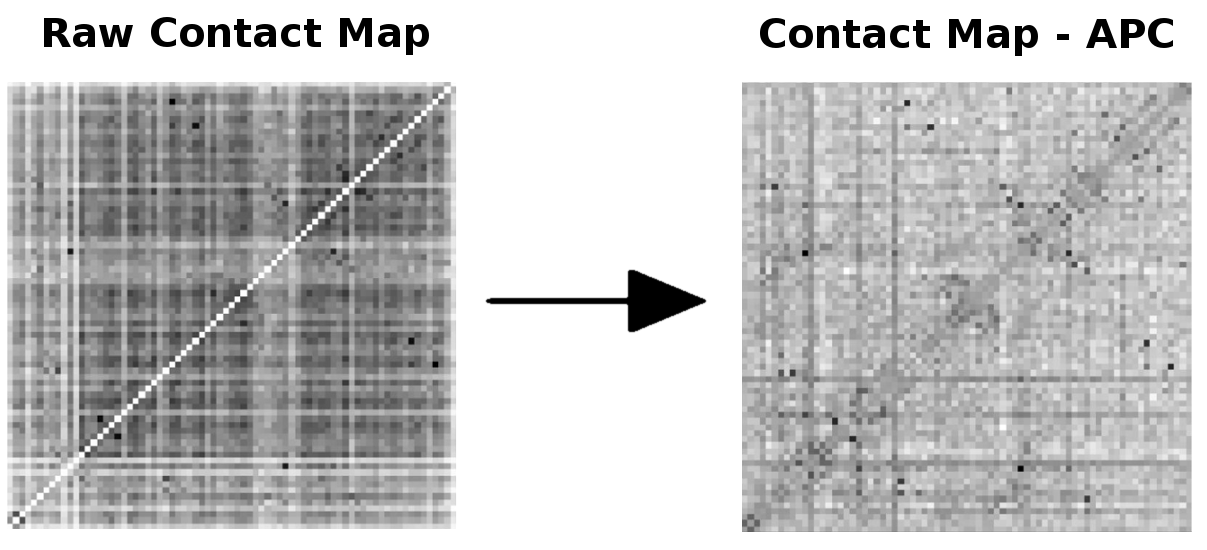
\includegraphics[width=1\linewidth]{img/intro/apc_correction_transparent} \caption{Contact Matrices computed from
pseudo-likelihood couplings. \textbf{a}: Contact map computed with
Frobenius norm as in eq. \eqref{eq:frobenius-norm}. Overall coupling
values are dominated by entropic effects, i.e.~the amount of variation
for a \protect\hyperlink{abbrev}{MSA} position, leading to striped
patterns. \textbf{b}: Contact map from (a) corrected for background
noise with the \protect\hyperlink{abbrev}{APC} as in eq. \eqref{eq:apc}.}\label{fig:apc-correction}
\end{figure}

\subsection{Challenges in Coevolutionary Inference}\label{challenges}

Coevolutionary methods face several challenges when interpreting the
covariation signals obtained from \protect\hyperlink{abbrev}{MSA} that
will be addressed in the following. Some of these challenges have been
successfully met (e.g.~transitive effects with global statistical
models), others are still open and again others open up new
possibilities, such as dissecting different sources of coevolution.

\subsubsection*{Phylogenetic Bias}\label{phylogenetic-bias}
\addcontentsline{toc}{subsubsection}{Phylogenetic Bias}

Sequences in \protect\hyperlink{abbrev}{MSAs} do not represent
independent samples of a protein family. In fact, there is selection
bias from sequencing species of special interest (e.g human pathogens)
or sequencing closely related species, e.g multiple strains. This uneven
sampling of a protein family's sequence space thus leaves certain
regions unexplored whereas others are statistically overrepresented
{[}\protect\hyperlink{ref-Morcos2011}{53},\protect\hyperlink{ref-Marks2012}{69}{]}.

Furthermore, due to their evolutionary relationships, sequences have a
complicated dependence structure. Closely related sequences can cause
spurious correlations between positions, as there was not sufficient
time for the sequences to diverge from their common ancestor
{[}\protect\hyperlink{ref-Gouveia_Oliveira2007}{40},\protect\hyperlink{ref-Lapedes1999}{45},\protect\hyperlink{ref-Burger2010}{47}{]}.
Figure \ref{fig:phylogenetic-effect} illustrates a simplified example,
where dependence of sequences due to phylogeny leads to a covariation
signal.






\begin{figure}

{\centering 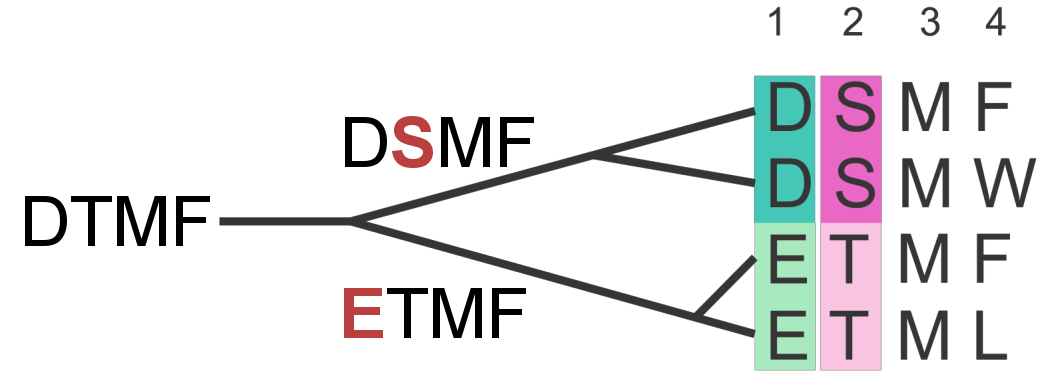
\includegraphics[width=0.5\linewidth]{img/intro/phylogenetic_effect} 

}

\caption{The phylogenetic dependence of closely
related sequences can produce covariation signals. Here, two independent
mutation events in two branches of the tree result in a perfect
covariation signal for two positions.}\label{fig:phylogenetic-effect}
\end{figure}

To reduce the effects of redundant sequences, a popular sequence
reweighting strategy has been found to improve contact prediction
performance, where every sequence receives a weight that is the inverse
of the number of similar sequences according to an identity threshold
(see section \ref{seq-reweighting})
{[}\protect\hyperlink{ref-Jones2012}{44},\protect\hyperlink{ref-Morcos2011}{53},\protect\hyperlink{ref-Buslje2009}{70}{]}.

\subsubsection*{Entropic bias}\label{entropic-bias}
\addcontentsline{toc}{subsubsection}{Entropic bias}

Another source for noise is entropy bias that is closely linked to
phylogenetic effects. By nature, methods detecting signals from
correlated mutations rely on a certain degree of covariation between
sequence positions {[}\protect\hyperlink{ref-Burger2010}{47}{]}. Highly
conserved interactions pose a conceptual challenge, as changes from one
amino acid to another cannot be detected if sequences do not vary. This
results in generally higher co-evolution signals from positions with
high entropy and underestimated signals for highly conserved
interactions {[}\protect\hyperlink{ref-Fodor2004}{38}{]}.

Several heuristics have been proposed to reduce entropy effects, such as
Row-Column-Weighting (RCW)
{[}\protect\hyperlink{ref-Gouveia_Oliveira2007}{40}{]} or Average
Product Correction (APC) {[}\protect\hyperlink{ref-Dunn2008}{29}{]} (see
section \ref{post-processing-heuristics}).

\subsubsection*{Finite Sampling Effects}\label{finite-sampling-effects}
\addcontentsline{toc}{subsubsection}{Finite Sampling Effects}

Spurious correlations can arise from random statistical noise and blur
true co-evolution signals especially in low data scenarios.
Consequently, false positive predictions attributable to random noise
accumulate for protein families comprising low numbers of homologous
sequences. This relationship was confirmed in many studies and as a rule
of thumb it has been argued that proteins with \(L\) residues need at
least \emph{5L} sequences in order to obtain confident predictions
useful for protein structure prediction
{[}\protect\hyperlink{ref-Kamisetty2013}{61},\protect\hyperlink{ref-Marks2012}{69}{]}.
Recently it was shown that precision of predicted contacts saturates for
protein families with more than \(10^3\) diverse sequences and that
precision is only dependent on protein length for families with small
number of sequences {[}\protect\hyperlink{ref-Anishchenko2017}{71}{]}.

Interesting targets for contact prediction are protein families without
any associated structural information. As can be seen in Figure
\ref{fig:pfam}, those protein families generally comprise low numbers of
homologous sequences with a median of 185 sequences per family and are
thus susceptible to finite sampling effects.

With the rapidly increasing size of protein sequence databases (see
section \ref{general-intro}) the number of protein families with enough
sequences for accuarate contact predictions will also increase steadily
{[}\protect\hyperlink{ref-TheUniProtConsortium2013}{11},\protect\hyperlink{ref-Kamisetty2013}{61}{]}.
Nevertheless, because of the already mentioned sequencing biases, better
and more sensitive statistical models are indespensible to extend the
applicability domain of coevolutionary methods.








\begin{figure}

{\centering 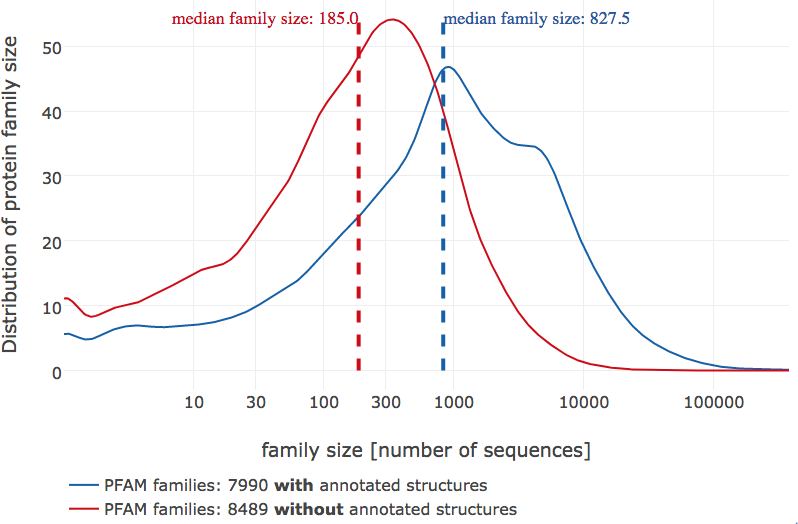
\includegraphics[width=0.9\linewidth]{img/pfam_pdb_notitle} 

}

\caption{Distribution of PFAM family sizes. Less than half of
the families in PFAM (7990 compared to 8489 families) do not have an
annotated structure. The median family size in number of sequences for
families with and without annotated structures is 185 and 827
respectively. Data taken from PFAM 31.0 (March 2017, 16712 entries)
{[}\protect\hyperlink{ref-Finn2016}{72}{]}.}\label{fig:pfam}
\end{figure}

\hypertarget{transitive-effects}{\subsubsection*{Transitive
Effects}\label{transitive-effects}}
\addcontentsline{toc}{subsubsection}{Transitive Effects}

One important shortcoming of traditional covariance approaches arises
from the fact that chains of amino acid interactions are very common in
protein structures and lead to direct as well as indirect correlation
signals
{[}\protect\hyperlink{ref-Weigt2009}{30},\protect\hyperlink{ref-Lapedes1999}{45},\protect\hyperlink{ref-Burger2010}{47}{]}.

Considering three residues \(i\), \(j\) and \(k\), where \(i\) interacts
with \(j\) and \(j\) interacts with \(k\). Even when there is no
physical interaction between \(i\) and \(k\), there will be a
correlation between \(i\) and \(k\) due to the correlation versus
causation phenomenon. Strong statistical dependence between pairs
\((i,j)\) and \((j,k)\) can induce strong indirect signals which can be
even larger than signals of other directly interacting pairs and thus
lead to false predictions {[}\protect\hyperlink{ref-Burger2010}{47}{]}.

Local statistical methods, being introduced in section
\ref{local-methods}, are unable to disentangle these transitive effects
as they consider residue pairs independent of one another. In contrast,
global statistical models presented in section \ref{global-methods}
learn a joint probability over all residues allowing to dissect direct
and indirect correlations
{[}\protect\hyperlink{ref-Weigt2009}{30},\protect\hyperlink{ref-Burger2010}{47}{]}.

\subsubsection*{Multiple Sequence
Alignments}\label{multiple-sequence-alignments}
\addcontentsline{toc}{subsubsection}{Multiple Sequence Alignments}

Obviously, a correct \protect\hyperlink{abbrev}{MSA} is the essential
starting point for correlated mutation analysis as incorrectly aligned
residues will confound the true covariation signal. Highly sensitive and
accurate tools such as HHblits generate high quality alignments suitable
for contact prediction {[}\protect\hyperlink{ref-Remmert2012}{73}{]}.
However, there are certain subtleties to be kept in mind when generating
alignments.

For example, proteins with repeated stretches of amino acids or with
regions of low complexity are notoriously hard to align. Especially,
repeat proteins have been found to account for a considerable fraction
of false positive predictions
{[}\protect\hyperlink{ref-Anishchenko2017}{71}{]}. Therefore,
\protect\hyperlink{abbrev}{MSAs} need to be generated with great care
and covariation methods need to be tailored to these specific problems
{[}\protect\hyperlink{ref-Espada2014}{74},\protect\hyperlink{ref-Toth-Petroczy2016}{75}{]}.

Sensitivity of sequence search is critically dependent on the research
question and the protein family of interest. While many diverse
sequences generally increase precision of predictions, co-evolutionary
signals specific to a subfamily might be averaged out when alignments
become too deep. Therefore a trade-off between specificity and diversity
of the alignment is required to reach optimal results
{[}\protect\hyperlink{ref-Hopf2012}{76}{]}.

Another intrinsic characteristic of \protect\hyperlink{abbrev}{MSAs} are
repeated stretches of gaps that result from commonly utilized
gap-penalty schemes assigning large penalties to insert a gap and lower
penalties to gap extensions. Most statistical models treat gaps as the
21st amino acid, thus introducing an imbalance as gaps and amino acid
express different behaviours which often results in gap-induced
artefacts {[}\protect\hyperlink{ref-Feinauer2014}{67}{]}.

\subsubsection*{Evaluation Strategy}\label{evaluation-strategy}
\addcontentsline{toc}{subsubsection}{Evaluation Strategy}

Contact prediction methods are typically evaluated based on a rigid
definition of a residue contact as discussed in section
\ref{intro-cp-evaluation}.

However, whether two residues truly interact in a protein structure
depends only marginally on the distance between their \(\Cb\) atoms.
More importantly, interactions between side-chains depend on their
physico-chemical properties, on their orientation and vary within the
vast number of alternative environments within proteins
{[}\protect\hyperlink{ref-Bettsa}{77}{]} (see section
\ref{amino-acid-interactions}). Therefore, a simple \(\Cb\) distance
threshold cannot capture the true biological interaction preferences of
amino acids and yields an imperfect gold-standard for benchmarking.

Other distance thresholds or definitions for contacts (e.g minimal
atomic distances or distance between functional groups) have been
studied as well. In fact, Duarte and colleagues found that using a
\(\Cb\) distance threshold between 9\(\AA \; \;\) and 11\(\AA \; \;\)
yields optimal results when predicting the 3D structure from the
respective contacts {[}\protect\hyperlink{ref-Duarte2010}{78}{]}.

Anishchenko and colleagues
{[}\protect\hyperlink{ref-Anishchenko2017}{71}{]} analysed false
positive predictions with respect to a minimal atom distance threshold
\(< 5 \AA \; \;\), as they found that this cutoff optimally defines
direct physical interactions of residue pairs.

Therefore, choosing different distance cutoffs or different reference
atoms for defining a true contact changes the evaluation outcome. With
regard to the utilization of contacts for structure prediction, a simple
\(\Cb\) cutoff is nonetheless a convenient choice, as this threshold can
be easily implemented as a restraint in common structure predictions
protocols (e.g Modeller). Furthermore, \protect\hyperlink{abbrev}{CASP}
introduced the \(8\AA \; \; \Cb\) definition for a contact which has
become well established in the mean time.

Related to the problem of choosing the right trade-off between
sensitivity and specificity when generating alignemnts is the issue of
structural variation within a protein family. Evolutionary couplings are
inferred from all family memebers in the \protect\hyperlink{abbrev}{MSA}
and thus might be physical contacts in one family member but not in
another. Anishchenko et al. could show that more than \(80\%\) of false
positives at intermediate distances (minimal heavy atom distance
\(5-15 \AA \;\;\)) are true contacts in at least one homolog structure
{[}\protect\hyperlink{ref-Anishchenko2017}{71}{]}.

\subsubsection*{Alternative Sources of
Co-evolution}\label{alternative-sources-of-co-evolution}
\addcontentsline{toc}{subsubsection}{Alternative Sources of
Co-evolution}

Co-evolutionary signals can not only arise from intra-domain contacts,
but also from other sources, like homo-oligomeric contacts, alternative
conformations, ligand-mediated interactions or even contacts over
hetero-oligomeric interfaces (see Figure \ref{fig:sources-coevolution})
{[}\protect\hyperlink{ref-Marks2012}{69}{]}. With the objective to
predict physical contacts it is therefore necessary to identify and
filter these alternative sources for co-evolutionary couplings.








\begin{figure}

{\centering 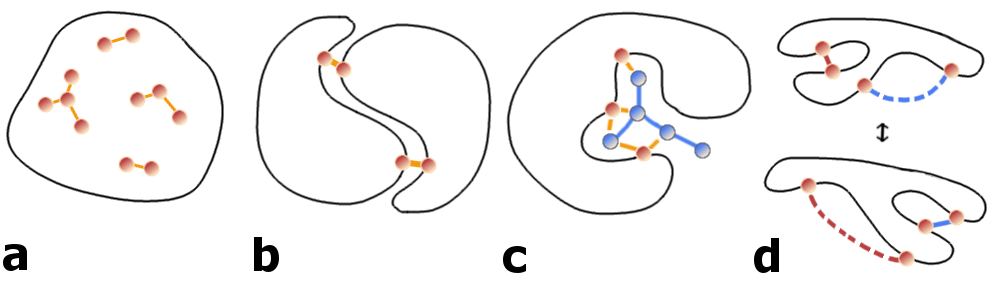
\includegraphics[width=0.8\linewidth]{img/intro/sources_of_coevolution} 

}

\caption{Possible causes of coevolution.
\textbf{a)} Physical interactions between intra-domain residues.
\textbf{b)} Interactions across the interface of predominantly
homo-oligomeric complexes. \textbf{c)} Interactions mediated by ligands
or metal atoms. \textbf{d)} Transient interactions due to conformational
flexibility.}\label{fig:sources-coevolution}
\end{figure}

Many proteins form homo-oligomers with evolutionary conserved
interaction surfaces. Currently it is hard to reliably distinguish
intra- and inter-molecular contacts. Anishchenko et al. found that
approximately one third of strong co-evolutionary signals between
residue pairs at long distances (minimal heavy atom distance
\(>15 \AA \;\;\)) can be attributed to interactions across
homo-oligomeric interfaces
{[}\protect\hyperlink{ref-Anishchenko2017}{71}{]}. Several studies
specifically analysed co-evolution across homo-oligomeric interfaces for
proteins of known structure by filtering for residue pairs with strong
couplings at long distances
{[}\protect\hyperlink{ref-Hopf2012}{76},\protect\hyperlink{ref-Lee2009}{79}--\protect\hyperlink{ref-Jana2014}{82}{]}
or used co-evolutionary signals to predict homo-dimeric complexes
{[}\protect\hyperlink{ref-DosSantos2015a}{83}{]}.

It has been proposed that co-evolutionary signals can also arise from
ligand or atom mediated interactions between residues or from critical
interactions in intermediate folding states
{[}\protect\hyperlink{ref-Buslje2009}{70},\protect\hyperlink{ref-Ovchinnikov2015b}{84}{]}.
Confirming this hypothesis, a study showed that the cumulative strength
of couplings for a particular residue can be used to predict functional
sites
{[}\protect\hyperlink{ref-Marks2012}{69},\protect\hyperlink{ref-Hopf2012}{76}{]}.

Another important aspect is conformational flexibility. PDB structures
used to evaluate co-evolution analysis represent only rigid snapshots
taken in an unnatural crystalline environment. Yet proteins possess huge
conformational plasticity and can adopt distinct alternative
conformations or adapt shape when interacting with other proteins in an
induced fit manner {[}\protect\hyperlink{ref-Noel2016}{85}{]}. Several
studies demonstrated successfully that co-evolutionary signals can
capture interactions specific to different distinct conformations
{[}\protect\hyperlink{ref-Morcos2011}{53},\protect\hyperlink{ref-Hopf2012}{76},\protect\hyperlink{ref-Jana2014}{82},\protect\hyperlink{ref-Sfriso2016}{86}{]}.

\section{Developing a Bayesian Model for Contact
Prediction}\label{developing-a-bayesian-model-for-contact-prediction}

The most popular and successfull methods for contact prediction optimize
the pseudo-log-likelihood of the \protect\hyperlink{abbrev}{MSA} and use
several heuristics to calculate a contact score (see section
\ref{post-processing-heuristics}).

By doing so valuable information in contact matrices is lost. Analyses
in section 1 shows what information is contained in coupling matrices
and that the signal in coupling matrices varies with \(\Cb\) distance.

This thesis introcudes a principled Bayesian statistical approach that
eradicates these heuristics to fully exploit the information in coupling
matrices. Instead of transforming the model parameters \(\w\) into
heuristic contact scores, one can compute the posterior probability
distributions of the distances \(r_{ij}\) between \(\Cb\) atoms of all
residues pairs \(i\) and \(j\), given the
\protect\hyperlink{abbrev}{MSA} \(\X\). The coupling parameters \(\w\)
are treated as hidden variables that will be integrated out
analytically. This approach also allows for extraction of information
contained in the particular types of amino acids, since each pair of
amino acids will have a different preference to be coupled at certain
distances.

TODO Figure ! !

In section 2 introduces max ent model for protein families that will
produce the model parameters for the Bayesian model.

In section 3 describes in detail how the posterior distribution of
distances can be computed.

Section 4 presents the optimizaton of the coupling prior.

And the Bayesian model will be evalutated in section 5.

The outlook describes an extension of the model to predict inter-residue
distances. Development is ongoing.

\chapter{Interpretation of Coupling
Matrices}\label{interpreting-coupling-matrices}

State-of-the-art contact prediction methods map the 20 x 20 coupling
matrices \(w_{ij}\) onto scalar values to obtain contact scores for each
residue pair (see section \ref{post-processing-heuristics}). By doing
so, the full information contained in coupling matrices is lost:

\begin{itemize}
\tightlist
\item
  the contribution of individual couplings \(\wijab\)
\item
  the direction of couplings (positive or negative)
\item
  the correlation between couplings \(\wijab\) and \(\wijcd\)
\item
  intrinsic biological meaning
\end{itemize}

The following analyses give some intuition for the information contained
in coupling matrices.

\section{Single Coupling Values Carry Evidence of
Contacts}\label{single-coupling-values-carry-evidence-of-contacts}

Given the success of \protect\hyperlink{abbrev}{DCA} methods, it is
clear that contact scores are good indicators of spatial proximity for
residue pairs. As described in section \ref{post-processing-heuristics},
a contact score for a residue pair is commonly computed as the square
root over the sum of squared coupling values.

Figure \ref{fig:sq-coupling-correlation} shows the correlation between
squared coupling values and contact class. All couplings have a positive
class correlation, meaning the stronger their squared value, the more
likely a contact can be inferred. Generally, couplings that involve any
aliphatic amino acid (I, L, V) or alanine express the strongest class
correlation. In contrast, C-C or aromatic pairings (involving Y, F, W)
correlate only weakly with contact class. Therefore, these couplings
often might contribute to false positive predictions.








\begin{figure}

{\centering 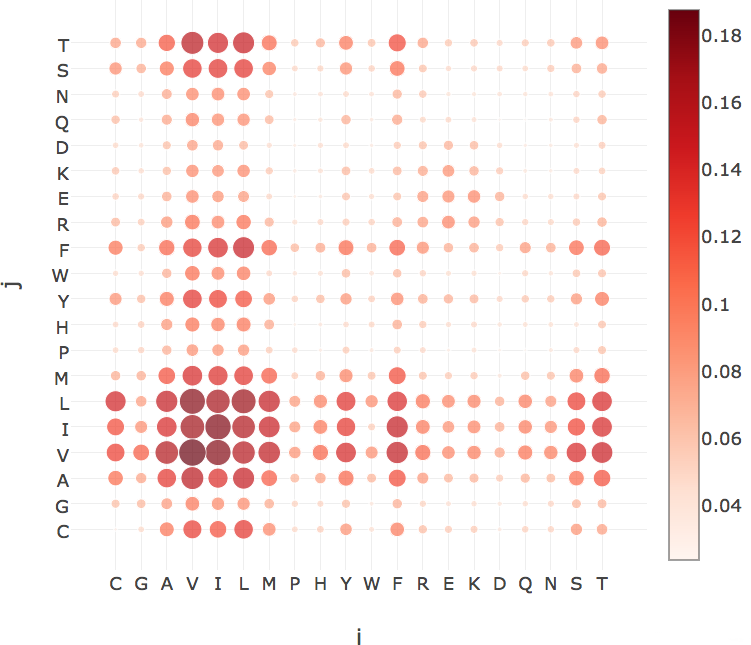
\includegraphics[width=0.9\linewidth]{img/coupling_matrix_analysis/correlation_squared_couplings_with_contact_class_notitle} 

}

\caption{Correlation of squared coupling values
\((\wijab)^2\) with contact class (contact=1, non-contact=0) for
approximately 100 000 residue pairs per class (details see section
\ref{method-coupling-correlation}). Contacts defined as residue pairs
with \(\Cb < 8 \AA\) and non-contacts as residue pairs with
\(\Cb > 25 \AA\).}\label{fig:sq-coupling-correlation}
\end{figure}

Apparantly, distinct couplings are of varying importance for contact
inference. Without squaring the coupling values, these charateristics
become even more pronounced.

Figure \ref{fig:coupling-correlation} shows the correlation of raw
coupling values with contact class. Interestingly, in contrast to the
finding with squared coupling values, only couplings for charged pairs
have strong correlation (positive and negative) with class value,
whereas couplings for hydrophobic pairs correlate to a much lesser
extent (mostly negative). This implies that absolute (squared) coupling
strength is much more indicative of a contact for hydrophobic pairings
than the direction of coupling. On the contrary, for charged residue
pairs the direction of a coupling value is a stronger indicator than the
strength of the squared coupling value.

As with squared couplings, raw couplings for aromatic pairs or C-C pairs
correlate only weakly with contact class. For these pairings, neither
coupling strength, nor direction of coupling seems to be a good
indicator for a contact.



\begin{figure}
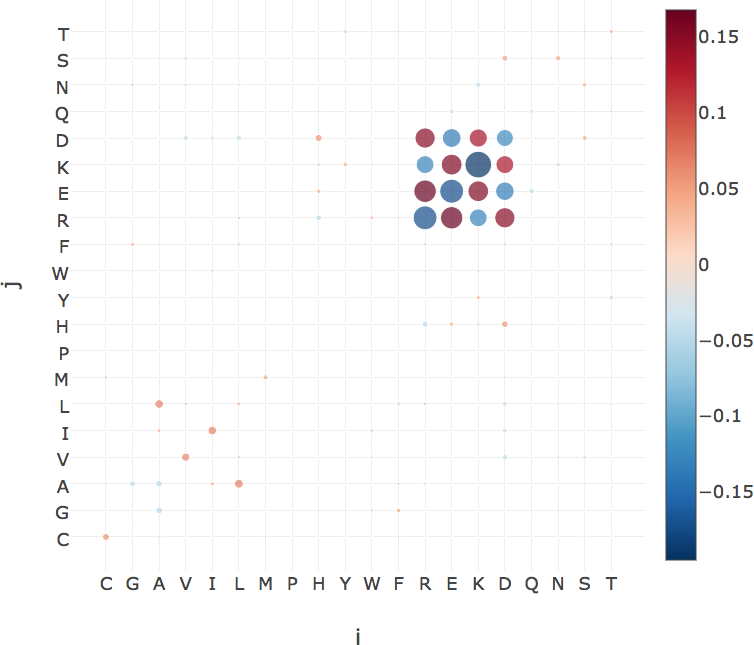
\includegraphics[width=0.9\linewidth]{img/coupling_matrix_analysis/correlation_couplings_with_contact_class_notitle} \caption{TODOOOOOOO.}\label{fig:coupling-correlation}
\end{figure}

Of course, looking only at correlations can be misleading if there are
non-linear patterns in the data, for example higher order dependencies
between couplings. For this reason it is advisable to take a more
detailed view at coupling matrices and the distributions of their
values.

\section{Physico-Chemical Fingerprints in Coupling
Matrices}\label{physico-chemical-fingerprints-in-coupling-matrices}

The correlation analysis of raw coupling matrices in the last section
revealed that certain coupling values tend to indicate a contact more
strongly than others. Single coupling matrices of residue contacts often
display striking patterns that agree with the previuos findings. Most
often, these patterns suggest biological relevant details of the
interdependency between both residues.

Figure \ref{fig:coupling-matrix-ionic-interaction} visualizes the
inferred coupling matrix for a residue pair (residues 6 and 82) in
protein 1awq, chain A. Clearly visible is a cluster of strong coupling
values for charged and polar residues (E,D,K,R,Q). Positive coupling
values can be observed between positively charged residues (R,K) and
negatively charged residues (E,D), whereas coupling values between
equally charged residues are negative. The coupling matrix perfectly
reflects the interaction preference for residues forming salt bridges.
Indeed, in the protein structure residue 6 (glutamic acid) forms a salt
bridge with residue 82 (lysine) as can be seen in figure
\ref{fig:coupling-matrix-pymol}.









\begin{figure}
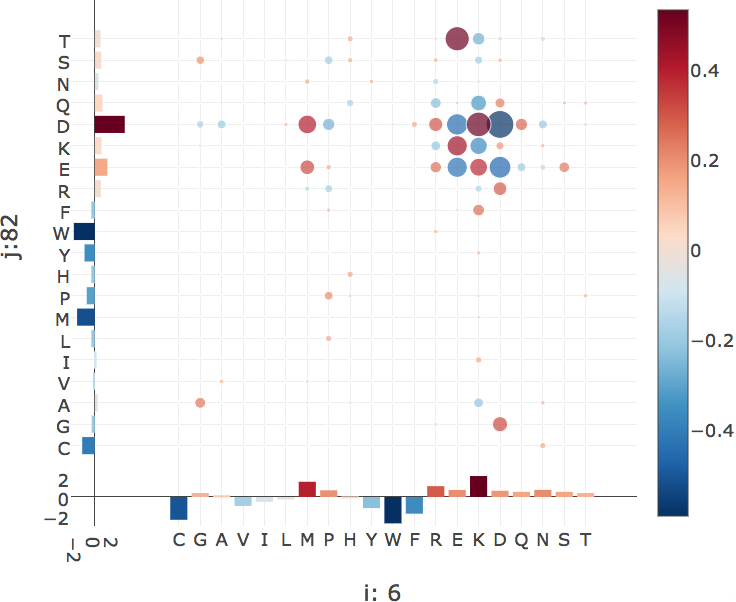
\includegraphics[width=0.9\linewidth]{img/coupling_matrix_analysis/coupling_matrix_1a9xA05_6_82_notitle} \caption{Coupling matrix for
residues 6 and 82 in protein 1awq chain A. Size of the bubbles
represents coupling strength and color represents the direction of
coupling: red = positive coupling, blue = negative coupling. Bars at the
x-axis and y-axis represent the corresponding single potentials for both
residues. Height of the bars represents potential strength and color
represents positive (red) and negative (blue) values.}\label{fig:coupling-matrix-ionic-interaction}
\end{figure}

Figure \ref{fig:coupling-matrix-hydrophobic-interaction} visualizes the
coupling matrix for a pair of hydrophobic residues (residues 29 and 39)
in protein 1ae9 chain A. Hydrophobic pairings have strong coupling
values but the couplings also reflect a sterical constraint: alanine as
a small hydrophobic residue is favoured at either position 29 or
position 39, but disfavoured to appear at both positions. Figure
\ref{fig:coupling-matrix-pymol} illustrates the location of the two
residues in the protein core. Here, hydrophobic residues are densely
packed and the limited space allows for only small hydrophobic residues.









\begin{figure}
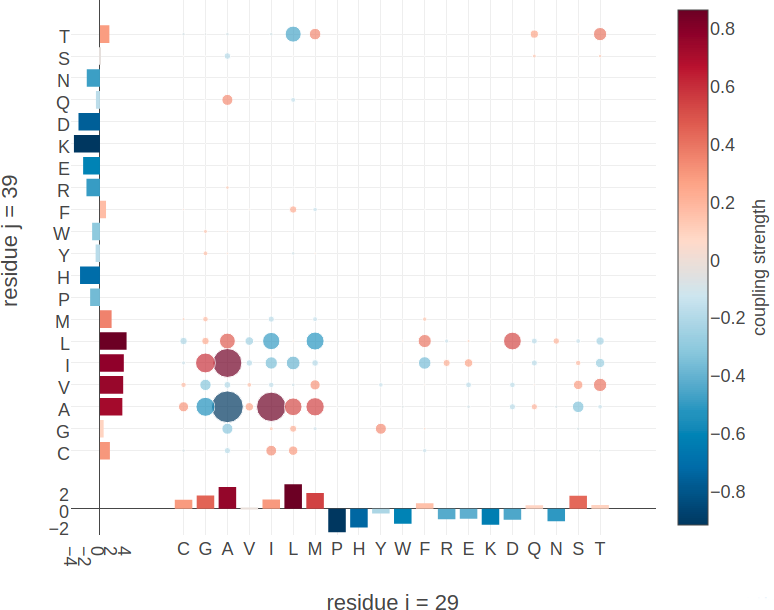
\includegraphics[width=0.9\linewidth]{img/coupling_matrix_analysis/coupling_matrix_1ae9A00_29_39_notitle} \caption{Coupling matrix
for residues 29 and 39 in protein 1ae9 chain A. Size of the bubbles
represents coupling strength and color represents the direction of
coupling: red = positive coupling, blue = negative coupling. Bars at the
x-axis and y-axis represent the corresponding single potentials for both
residues. Height of the bars represents potential strength and color
represents positive (red) and negative (blue) values.}\label{fig:coupling-matrix-hydrophobic-interaction}
\end{figure}







\begin{figure}
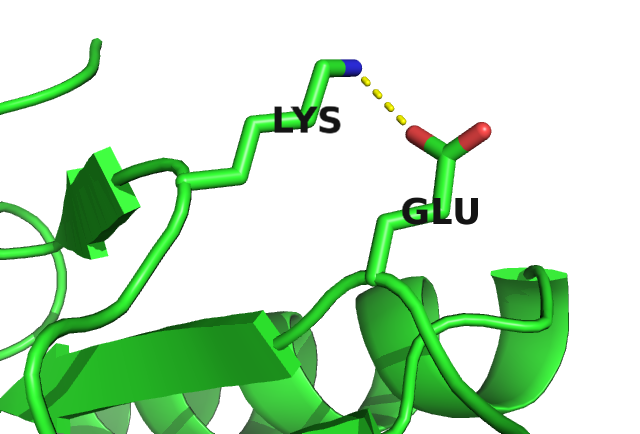
\includegraphics[width=0.5\linewidth]{img/coupling_matrix_analysis/1a9xA05_6_82} 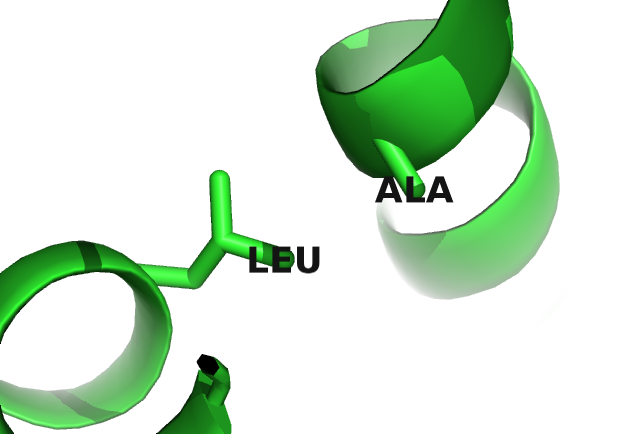
\includegraphics[width=0.5\linewidth]{img/coupling_matrix_analysis/1ae9A00_29_39} \caption{Interactions between protein side
chains. Left: residue 6 (glutamic acid) forming a salt bridge with
residue 82 (lysine) in protein 1awq, chain A. Right: residue 29
(alanine) and residue 39 (leucine) within the hydrophobic core of
protein 1ae9 chain A.}\label{fig:coupling-matrix-pymol}
\end{figure}

Many more biological interpretable signals can be identified from
coupling matrices, including pi-cation interactions (see Appendix
\ref{pi-cation}), aromatic-proline interactions (see Appendix
\ref{aromatic-proline}), sulfur-aromatic interactions or disulphide
bonds (see Appendix \ref{disulfide}).

Coucke and collegues {[}\protect\hyperlink{ref-Coucke2016}{87}{]}
performed a thorough quantitative analysis of coupling matrices selected
from confidently predicted residue pairs. They showed that eigenmodes
obtained from a spectral analysis of averaged coupling matrices are
closely related to physico-chemical properties of amino acid
interactions, like electrostaticity, hydrophobicity, steric interactions
or disulphide bonds. By looking at specific populations of residue
pairs, like buried and exposed residues or residues pairs from specific
protein classes (small, mainly \(\alpha\), etc), the eigenmodes capture
very characteristic interactions for each class, e.g.~rare disulfide
contacts withins small proteins and hydrophilic contacts between exposed
residues. Their study confirms our qualitative observation that amino
acid interactions can leave characteristic physico-chemical fingerprints
in coupling matrices.

\section{Coupling Profiles Vary with
Distance}\label{coupling-profiles-vary-with-distance}

Analyses in the previous sections showed that certain coupling values
correlate more or less strong with contact class and that coupling
matrices for contacts express biological meaningpull patterns.

More insights can be obtained by looking at the distribution of distinct
coupling values for contacts, non-contacts and arbitrary populations of
residue pairs. To avoid uninformative couplings, we consider only
residue pairs with a sequence separation \textgreater{} 10 and with
enough evidence for a certain amino acid pairing (see Methods section
\ref{method-coupling-profile} for details).

Figure \ref{fig:1d-coupling-profile-0-5} shows the distribution of
selected couplings for residue pairs within a \(\Cb\) distance
\(< 5\AA\). The distribution of R-E and E-E coupling values is shifted
and skewed towards positive and negative values respectively. This is in
accordance with attracting electrostatic interactions between the
positively charged side chain of arginine and the negatively charged
side chain of gluatamic acid and also with repulsive interactions
between the two negatively charged gluatamic acid side chains. Couling
values for C-C pairs have a broad distribution that is skewed towards
positive values, reflecting the strong signals obtained from covalent
disulphide bonds. Hydrophobic pairs like V-I have an almost symmetric
coupling distribution, confirming the finding that the direction of
coupling is not indicative of a true contact whereas the strength of the
coupling is. Hydrophobic interactions arising from the hydrophobic
effect are not specific or directed and can easily be substituted by
other hydrophobic residues, which explains the not very pronounced
positive coupling signal compared to more specific interactions, e.g
ionic interactions. The distribution of aromatic coupling values like
F-W is slightly skewed towards negative values, accounting for steric
hindrance of their large side chains at small distances.






\begin{figure}

{\centering 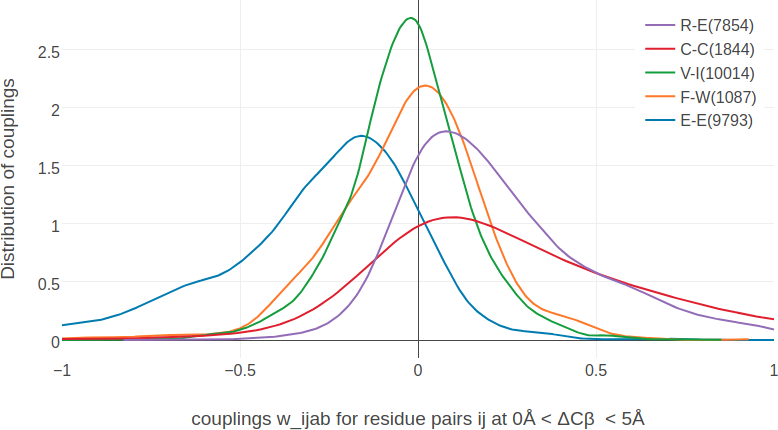
\includegraphics[width=0.9\linewidth]{img/coupling_matrix_analysis/1d_coupling_profile_0_5} 

}

\caption{Distribution of selected couplings
for approximately 10000 filtered residue pairs (value in brackets) with
\(\Cb\) distance \(< 5\AA \; \;\) (see Methods section
\ref{method-coupling-profile} for details).}\label{fig:1d-coupling-profile-0-5}
\end{figure}

In an intermediate \(\Cb\) distance range between \(8\AA\) and \(12\AA\)
the distributions for all coupling values are centered close to zero and
are less broad. The distributions are still shifted and skewed as for
\(\Cb\) distance \(< 5\AA\) but much less pronounced. For aromatic pairs
like F-W, the distribution of coupling values has very long tails,
suggesting strong couplings for aroamtic side chains at this distance.






\begin{figure}
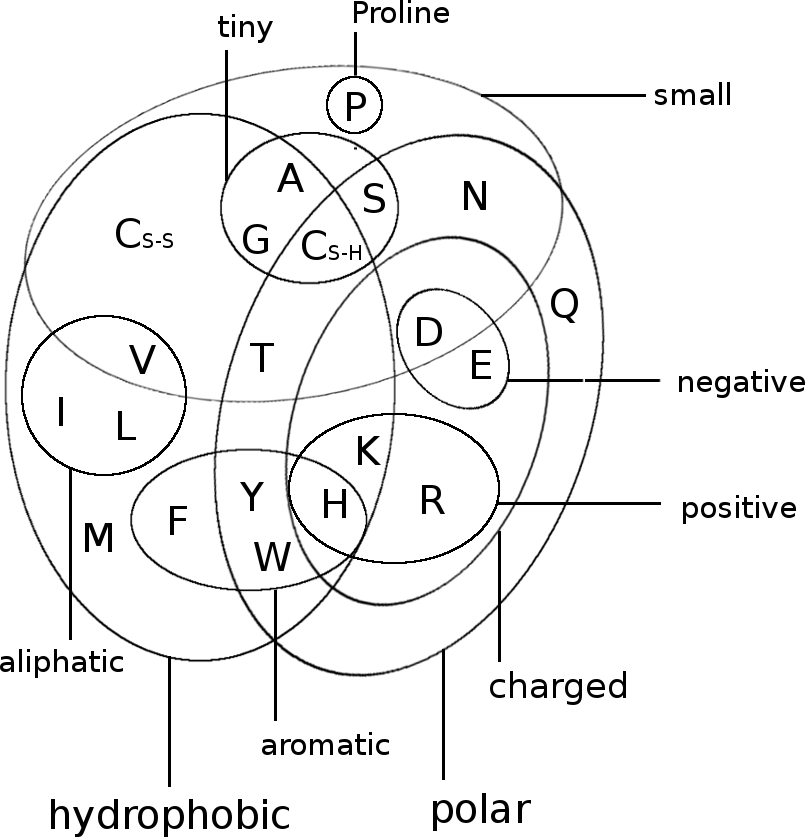
\includegraphics[width=1\linewidth]{img/amino_acid_physico_chemical_properties_venn_diagramm} \caption{Distribution of selected
couplings for approximately 10000 filtered residue pairs with \(\Cb\)
distance \(< 5\AA\) (see Methods section \ref{method-coupling-profile}
for details).}\label{fig:1d-coupling-profile-8-12}
\end{figure}

Figure \ref{fig:1d-coupling-profile-20-50} shows the distribution of
selected couplings for residue pairs far apart in the protein structure
(\(\Cb\) distance \(> 20\AA\)).\\
The distribution for all couplings is centered at zero and has small
variance. For C-C coupling values, the distribution has a long tail for
positve values, presumably arising from the fact that the maximum
entropy model cannot distuinguish highly conserved signals of multiple
disulphide bonds within a protein. This observation also agrees with the
previous finding that C-C couplings correlate only weakly with contact
class. The same arguments apply to couplings of aromatic pairs that have
a comparably broad distribution and do not correlate strongly with
contact class. The strong coevolution signals for aromatic pairs even at
high distance ranges might be to insufficient disentanglig of transitive
effects, as aromatic residues are known to form network-like structures
in the protein core that stabilize protein structure (see Figure
\ref{fig:aromatic-network} in
Appendix){[}\protect\hyperlink{ref-Burley1985}{13}{]}.






\begin{figure}
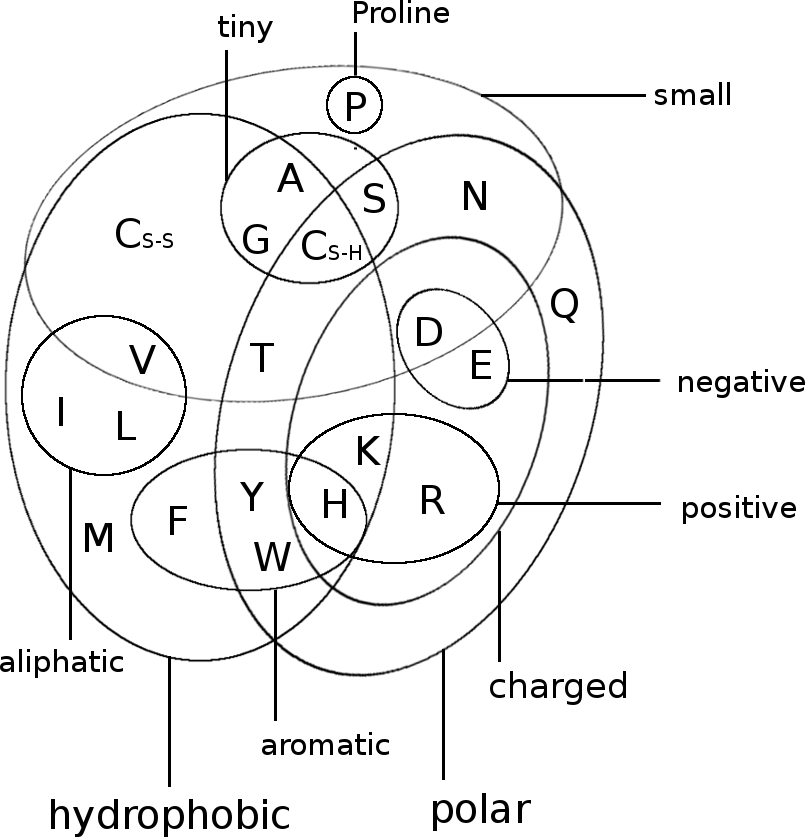
\includegraphics[width=1\linewidth]{img/amino_acid_physico_chemical_properties_venn_diagramm} \caption{Distribution of selected
couplings for approximately 10000 filtered residue pairs with \(\Cb\)
distance \(> 25\AA\) (see Methods section \ref{method-coupling-profile}
for details).}\label{fig:1d-coupling-profile-20-50}
\end{figure}

\section{Higher Order Dependencies Between
Couplings}\label{higher-order-dependencies-between-couplings}

The analyses in the previous sections focused on single coupling values
of the \(20 \times 20\)-dimensional coupling matrices. As mentioned
before, looking at single variables might be misleading if they are
dependent on another. Unfortunately, it is not possible to reasonably
visualize the high dimensional coupling matrices. But there are several
ways to identify interesting dimensions.

First of all, 2-dimensional scatter plots of couplings for biological
relevant pairings confirm the previous trend that couplings reflect
amino acid interactions.

Figure \ref{fig:2d-coupling-profile-re-er-0-8} and
\ref{fig:2d-coupling-profile-re-ee-0-8} illustrate the distribution of
attractive and repulsive ionic interactions at \(\Cb\) distances less
than \(8\AA\). Whereas coupling values for R-E and E-R are positively
correlated, coupling values for R-E and E-E are negatively correlated.
Hydrophobic coupling values for residue pairs at \(\Cb\) distances less
than \(8\AA\) are symmetrically distributed around zero, in agreement
with all previous analyses (Figure
\ref{fig:2d-coupling-profile-vi-il-0-8}).








\textbackslash{}begin\{figure\}
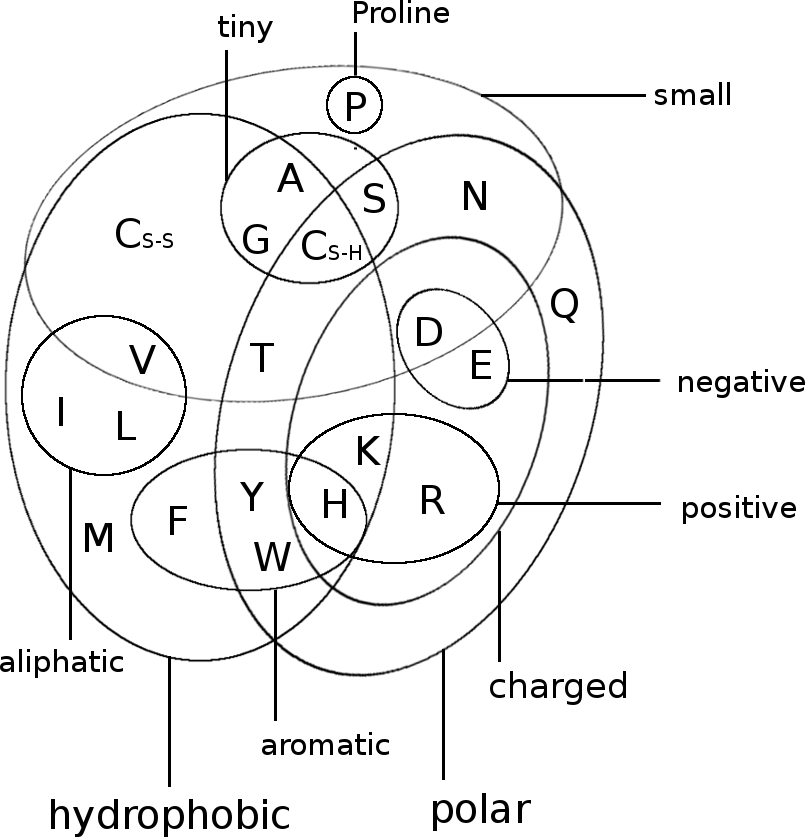
\includegraphics[width=0.75\linewidth]{img/amino_acid_physico_chemical_properties_venn_diagramm}








\begin{figure}
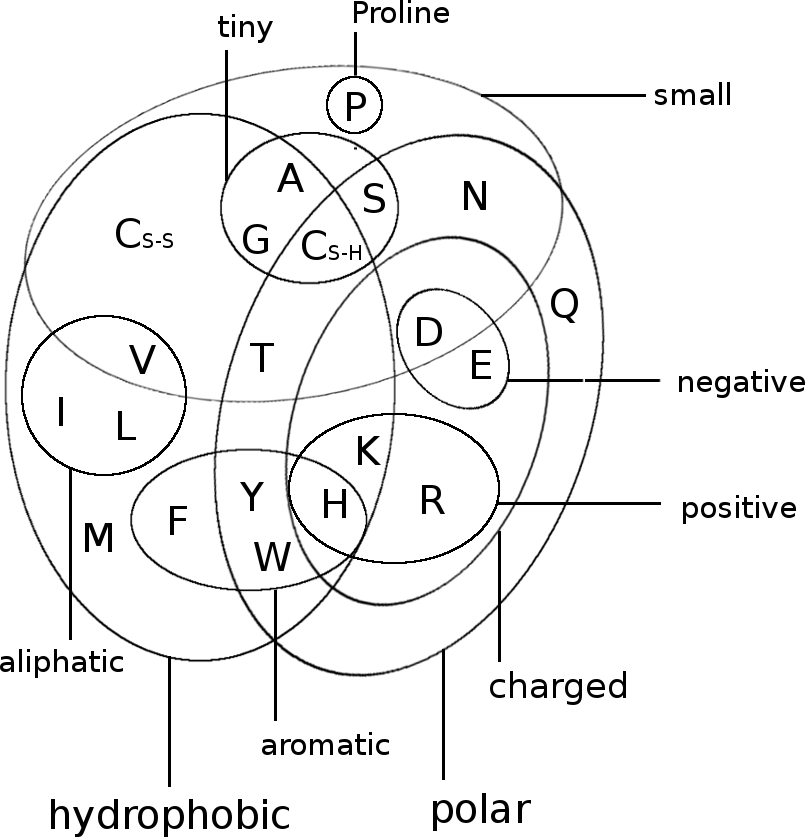
\includegraphics[width=0.75\linewidth]{img/amino_acid_physico_chemical_properties_venn_diagramm} \caption{Two-dimensional distribution
of coupling values R-E and E-E for approximately 10000 residue pairs
with \(\Delta\Cb < 8\AA\). The coupling values are negatively
correlated. Residue paris have been filtered for sequence separation,
percentage of gaps and evidence in alignment (see Methods
\ref{method-coupling-profile}).}\label{fig:2d-coupling-profile-re-ee-0-8}
\end{figure}








\begin{figure}
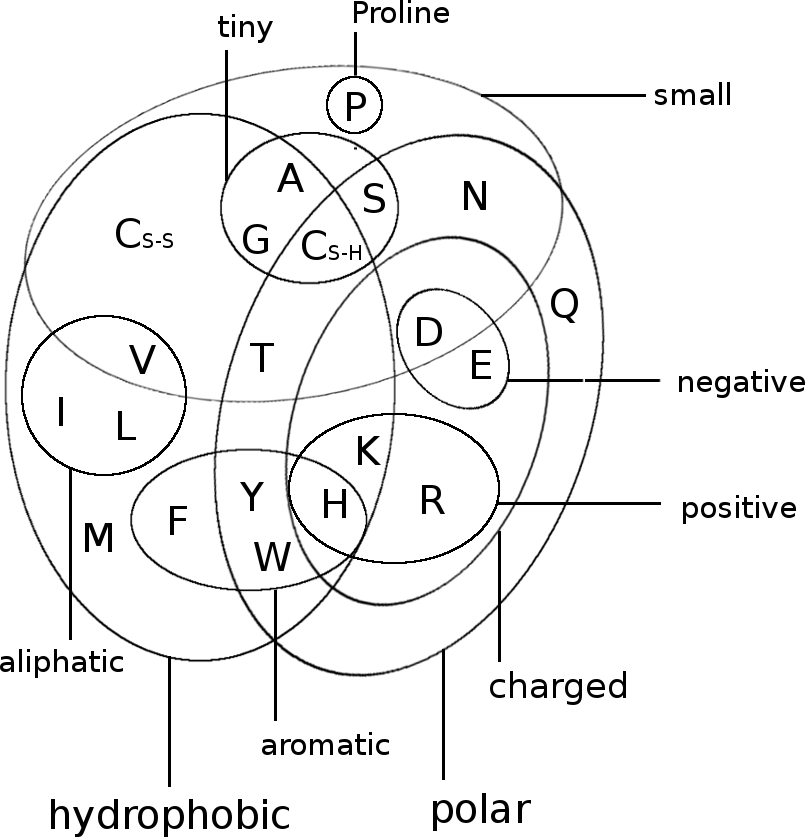
\includegraphics[width=0.75\linewidth]{img/amino_acid_physico_chemical_properties_venn_diagramm} \caption{Two-dimensional distribution
of coupling values V-I and I-L for approximately 10000 residue pairs
with \(\Delta\Cb < 8\AA\). The coupling values are symmetrically
distributed around zero. Residue paris have been filtered for sequence
separation, percentage of gaps and evidence in alignment (see Methods
\ref{method-coupling-profile}).}\label{fig:2d-coupling-profile-vi-il-0-8}
\end{figure}

\chapter{Optimizing the
Full-Likelihood}\label{optimizing-full-likelihood}

\section{Likelihood of the sequences as a Potts
model}\label{likelihood-of-the-sequences-as-a-potts-model}

We denote the \(N\) sequences in the \protect\hyperlink{abbrev}{MSA}
\(\X\) with \({\seq_1, ..., \seq_N}\). Each sequence
\(\seq_n = (\seq_{n1}, ..., \seq_{nL})\) is a string of \(L\) letters
from an alphabet indexed by \(\{0, ..., 20\}\), where 0 stands for a gap
and \(\{1, ... , 20\}\) stand for the 20 types of amino acids. The goal
is to predict from \(\X\) the distances \(r_{ij}\) between the \(\Cb\)
atoms of all pairs of residues \((i, j) \in \{1, ..., L\}\). The link
between the \protect\hyperlink{abbrev}{MSA} \(\X\) and the vector
\(\mathbf{r}\) of all inter-\(\Cb\) distances is described via the
evolutionary couplings of residue pairs that are the
\(20^2\)-dimensional vectors \(w_{ij}\).

As already described in detail in section \ref{maxent}, we model the
likelihood of the sequences in an \protect\hyperlink{abbrev}{MSA} with a
Potts Model, also known as \protect\hyperlink{abbrev}{MRF}:

\begin{equation}
    p(\X | \v, \w) = \prod_{n=1}^N p(\seq_n | \v, \w) = \prod_{n=1}^N \frac{1}{Z(\v, \w)} \exp \left( \sum_{i=1}^L v_i(x_{ni}) \sum_{1 \leq i < j \leq L} w_{ij}(x_{ni}, x_{nj}) \right)
\end{equation}

The coefficients \(\via\) are the single potentials and \(\wijab\)
denote the coupling strengths for pairs of residues. \(Z(\v, \w)\) is
the so-called partition sum that normalizes the probability distribution
\(p(\seq_n |\v, \w)\):

\begin{equation}
  Z(\v, \w) = \sum_{y_1, ..., y_L = 1}^{20} \exp \left( \sum_{i=1}^L v_i(y_i) \sum_{1 \leq i < j \leq L} w_{ij}(y_i, y_j)  \right)
\end{equation}

TODO: this is irrelevant for CD, isn't it? For an efficient
computational implementation, we might sum over all \(1 \le i, j \le L\)
without demanding \(i < j\) and enforce trivial constraints
\(\wijab = w_{jiba}\) during the optimization.

\section{Treating Gaps as Missing Information}\label{gap-treatment}

Treating gaps explicitly as 0'th letter of the alphabet would lead to
couplings between columns that are not in physical contact. To see why,
imagine a hypothetical alignment consisting of two sets of sequences as
it is illustrated in Figure \ref{fig:gap-treatment}. The first set has
sequences covering only the left half of columns in the MSA, while the
second set has sequences covering only the right half of columns. The
two blocks could correspond to protein domains that were aligned to a
single query sequence.

Now consider couplings between a pair of columns \(i, j\) with \(i\)
from the left half and \(j\) from the right half. Since no sequence
(except the single query sequence) overlaps both domains, the empirical
amino acid pair frequencies \(q(x_i = a, x_j = b)\) will vanish for all
\(a, b \in \{1,... , L\}\).










\begin{figure}
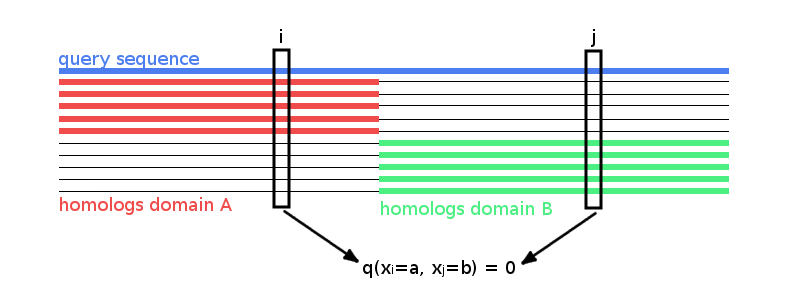
\includegraphics[width=11.11in]{img/gap_treatment} \caption{Hypothetical \protect\hyperlink{abbrev}{MSA}
consisting of two sets of sequences: the first set has sequences
covering only the left half of columns, while the second set has
sequences covering only the right half of columns. The two blocks could
correspond to protein domains that were aligned to a single query
sequence. Empirical amino acid pair frequencies
\(q(x_i \eq a, x_j \eq b)\) will vanish for positions \(i\) from the
left half and \(j\) from the right half of the alignment.}\label{fig:gap-treatment}
\end{figure}

The gradient of the log likelihood for couplings is

\begin{align}
\frac{\partial LL}{\partial \wijab} &= \sum_{n=1}^N I(x_{ni}=a, x_{nj}=b)  - N \frac{\partial}{\partial \wijab} \log Z(\v,\w) \\
                                        &= \sum_{n=1}^N I(x_{ni} \eq a, x_{nj} \eq b) \\
                                        & - N \sum_{y_1,\ldots,y_L=1}^{20} \!\! \frac{ \exp \left( \sum_{i=1}^L v_i(y_i) + \sum_{1 \le i < j \le L} w_{ij}(y_i,y_j) \right)}{Z(\v,\w)}  I(y_i \eq a, y_j \eq b) \\
                                        &=  N q(x_{i} \eq a, x_{j} \eq b) - N \sum_{y_1,\ldots,y_L=1}^{20} p(y_1, \ldots, y_L | \v,\w) \, I(y_i \eq a, y_j \eq b) \\
                                        &=  N q(x_{i} \eq a, x_{j} \eq b) - N p(x_i \eq a, x_j \eq b | \v,\w) 
\label{eq:gradient-LLreg-gaps-single}
\end{align}

Note that the empirical frequencies are equal to the model probabilities
at the maximum of the likelihood when the gradient vanishes. Therefore,
\(p(x_i \eq a, x_j \eq b | \v, \w)\) would have to be zero in the
optimum when the empirical amino acid frequencies
\(q(x_i \eq a, x_j \eq b)\) vanish for pairs of columns as described
above. However, \(p(x_i \eq a, x_j \eq b | \v, \w)\) can only become
zero, when the exponential term in \(p(x_i \eq a, x_j \eq b | \v, \w)\)
ammounts to zero, which would only be possible if \(\wijab\) goes to
\(−\infty\). This is clearly undesirable, as we want to deduce physical
contacts from the size of the couplings.

The solution is to treat gaps as missing information. This means that
the normalisation of \(p(\seq_n | \v, \w)\) should not run over all
positions \(i \in \{1,... , L\}\) but only over those \(i\) that are not
gaps in \(\seq_n\). Therefore we define the set of sequences \(\Sn\)
used for normalization of \(p(\seq_n | \v, \w)\) as:

\begin{equation}
\Sn := \{(y_1,... , y_L): 0 \leq y_i \leq 20 \land (y_i \eq 0 \textrm{ iff } x_{ni} \eq 0) \}
\end{equation}

and the partition function becomes:

\begin{equation}
  Z_n(\v, \w) = \sum_{\mathbf{y} \in \Sn} \exp \left( \sum_{i=1}^L v_i(y_i) \sum_{1 \leq i < j \leq L} w_{ij}(y_i, y_j)  \right)
\end{equation}

To ensure that the gaps in \(x_n\) do not contribute anything to the
sums, we fix all parameters associated with a gap to 0:

\(v_i(0) = 0\) and \(w_{ij}(0, b) = w_{ij}(a, 0) = 0\) for all
\(i, j \in \{1, ..., L\}\) and \(a, b \in \{0, ..., 20\}\).

Furthermore, we redefine the empirical amino acid frequencies \(q_{ia}\)
and \(q_{ijab}\) such that they are normalised over \(\{1, ..., 20\}\):

\begin{align}
   N_i :=& \sum_{n=1}^N  I(x_{ni} \!\ne\! 0) &  q_{ia} = q(x_i \eq a) :=& \frac{1}{N_i} \sum_{n=1}^N I(x_{ni} \eq a)   \\
   N_{ij} :=& \sum_{n=1}^N  I(x_{ni} \!\ne\! 0, x_{nj} \!\ne\! 0)  &  q_{ijab} = q(x_i \eq a, x_j \eq b) :=& \frac{1}{N_{ij}} \sum_{n=1}^N I(x_{ni} \eq a, x_{nj} \eq b)
\end{align}

With this definition, empirical amino acid frequencies are normalized
without gaps, so that

\begin{equation}
    \sum_{a=1}^{20} q_{ia} = 1      \; , \;     \sum_{a,b=1}^{20} q_{ijab} = 1.
\label{eq:normalized-emp-freq}
\end{equation}

\section{Gauge transformation}\label{gauge-transformation}

The model contains \(L \times 20 + \frac{L(L − 1)}{2} \times 20^2\)
parameters, but the parameters are not uniquely determined. For example,
for any fixed position \(i\) and amino acid a we can add a constant to
\(\via\) and subtract the same constant from the \(20L\) coefficients
\(\wijab\) with \(b \in \{1, ..., 20\}\) and \(j \in \{1, ..., L\}\).
This overparametrization, the so-called gauge transformation, would
leave the probabilities for all sequences under the model unchanged.

We could eliminate parameters by enforcing the restraints
\(\sum_{a=1}^{20} v_{ia} = 0\) and
\(\sum_{a=1}^{20} \wijab = 0 = \sum_{a=1}^{20} w_{ijba}\). However, it
is easier to rather formulate carefully the link between the
distribution of \(\w_{ij}\) vectors and the distance \(r_ij\) while
taking the non-uniqueness of parameters into acount, as we will see
below.

\section{The regularized log likelihood function
LLreg(v,w)}\label{the-regularized-log-likelihood-function-llregvw}

In pseudo-likelihood based methods, a regularisation is commonly used
that can be interpreted to arise from a prior probability. We will do
the same here, constraining \(\v\) and \(\w\) by Gaussian priors
\(\mathcal{N}( \v | \v^*, \lambda_v^{-1} \I)\) and
\(\mathcal{N}( \w |\boldsymbol 0, \lambda_w^{-1} \I)\). The choice of
\(v^*\) will be discussed in the section \ref{prior-v}. By including the
logarithm of this prior into the log likelihood using the gap treatment
described in section @ref\{gap-treatment\}, we obtain the regularised
likelihood,

\begin{equation}
    \LLreg(\v,\w)  = \log \left[ p(\X | \v,\w) \;  \Gauss (\v | \v^*, \lambda_v^{-1} \I)  \; \Gauss( \w | \boldsymbol 0, \lambda_w^{-1} \I) \right] 
\end{equation}

or explicitely,

\begin{align}
    \LLreg(\v,\w) =& \sum_{n=1}^N  \left[ \sum_{i=1}^L v_i(x_{ni}) + \sum_{1\le i<j\le L} w_{ij}(x_{ni},x_{nj}) - \log Z_n(\v,\w) \right] \\
                    & - \frac{\lambda_v}{2} \!\! \sum_{i=1}^L \sum_{a=1}^{20} (\via - \via^*)^2  - \frac{\lambda_w}{2}  \sum_{1 \le i < j \le L} \sum_{a,b=1}^{20} \wijab^2 .
\end{align}

\section{The gradient of the regularized log
likelihood}\label{the-gradient-of-the-regularized-log-likelihood}

The gradient of the regularized log likelihood has single components

\begin{align}
    \frac{\partial \LLreg}{\partial \via} =& \sum_{n=1}^N I(x_{ni}=a) - \sum_{n=1}^N \frac{\partial}{\partial \via} \, \log Z_n(\v,\w) - \lambda_v (\via - \via^*)\\
                                          =& \; N_i q(x_i \eq a) \\
                                          & - \sum_{n=1}^N \sum_{\mathbf{y} \in \Sn} \frac{  \exp \left( \sum_{i=1}^L v_i(y_i) + \sum_{1 \le i<j \le L}^L w_{ij}(y_i,y_j) \right) }{Z_n(\v,\w)}  I(y_i=a) \\
                                          & - \lambda_v (\via - \via^*) 
\label{eq:gradient-LLreg-single}
\end{align}

and pair components

\begin{align}
    \frac{\partial \LLreg}{\partial \wijab} =& \sum_{n=1}^N I(x_{ni} \eq a, x_{nj} \eq b) - \sum_{n=1}^N \frac{\partial}{\partial \wijab} \log Z_n(\v,\w)  - \lambda_w \wijab \\
                                            =& \; N_{ij} q(x_i \eq a, x_j=b) \\
                                            & - \sum_{n=1}^N \sum_{\mathbf{y} \in \Sn} \frac{ \exp \left( \sum_{i=1}^L v_i(y_i) + \sum_{1 \le i<j \le L}^L w_{ij}(y_i,y_j) \right) }{Z_n(\v,\w)} I(y_i \eq a, y_j \eq b) \\
                                            & - \lambda_w \wijab  
\label{eq:gradient-LLreg-pair}
\end{align}

Note that (without regulariation \(\lambda_v = \lambda_w = 0\)) the
empirical frequencies \(q(x_i \eq a)\) and \(q(x_i \eq a, x_j=b)\) are
equal to the model probabilities at the maximum of the likelihood.

If the proportion of gap positions in \(\X\) is small (e.g. \(<5\%\),
also compare percentage of gaps in dataset in Appendix Figure
\ref{fig:dataset-gaps}), we can approximate the sums over
\(\mathbf{y} \in \Sn\) in eqs. \eqref{eq:gradient-LLreg-single} and
\eqref{eq:gradient-LLreg-pair} by \(p(x_i=a | \v,\w) I(x_{ni} \ne 0)\) and
\(p(x_i=a, x_j=b | \v,\w) I(x_{ni} \ne 0, x_{nj} \ne 0)\), respectively,
and the partial derivatives become

\begin{align}
  \frac{\partial \LLreg}{\partial \via}   =& \; N_i q(x_i \eq a) -  N_i \; p(x_i \eq a  | \v,\w)  - \lambda_v (\via - \via^*)  \\
  \frac{\partial \LLreg}{\partial \wijab} =& \; N_{ij} q(x_i \eq a, x_j=b) - N_{ij} \; p(x_i \eq a, x_j \eq b | \v,\w) - \lambda_w \wijab
  \label{eq:gradient-LLreg-approx}
\end{align}

Note that the couplings between columns \(i\) and \(j\) in our
hypothetical MSA (see section \ref{gap-treatment}) will now vanish since
\(N_{ij} \eq 0\) and the gradient with respect to \(\wijab\) is equal to
\(-\lambda_w \wijab\).

\section{\texorpdfstring{The prior on
\(\v\)}{The prior on \textbackslash{}v}}\label{prior-v}

Most previous approaches chose a prior around the origin,
\(p(\v) = \Gauss ( \v| \mathbf{0}, \lambda_v \I)\). This choice has an
obvious draw-back. To see why, we take the sum over \(b=1,\ldots, 20\)
of the gradient of couplings in eq. \eqref{eq:gradient-LLreg-approx} at
the optimum, where the gradient vanishes.

This yields

\begin{equation}
    0 =   N_{ij}\, q(x_i \eq a, x_j \ne 0)   - N_{ij}\, p(x_i \eq a | \v, \w)  - \lambda_w \sum_{b=1}^{20} \wijab.
\end{equation}

Incidentally, we note that by taking the sum over \(a\) we find

\begin{equation}
    \sum_{a,b=1}^{20} \wijab  = 0.
\label{eq:zero-sum-wij}
\end{equation}

At the optimum the gradient with respect to \(v_{ia}\) vanishes and we
can substitute
\(p(x_i=a|\v,\w) = q(x_i=a) - \lambda_v (\via - \via^*) / N_i\),
yielding

\begin{equation}
    0 =  N_{ij} \, q(x_i \eq a, x_j \ne 0)  - N_{ij} \, q(x_i=a) + \frac{N_{ij}}{N_i}\lambda_v (\via - \via^*)  - \lambda_w \sum_{b=1}^{20} \wijab .
\label{eq:gauge-opt-1}
\end{equation}

for all \(i,j \in \{1,\ldots,L\}\) and all \(a \in \{1,\ldots,20\}\). To
show that the choice \(\v^*= \mathbf{0}\) leads to undesirable results,
we take an \protect\hyperlink{abbrev}{MSA} without gaps. The first two
terms \(N_{ij} \, q(x_i \eq a, x_j \ne 0) - N_{ij} \, q(x_i=a)\) vanish
as they add up to zero, which leaves

\begin{equation}
    0 =  \lambda_v (\via - \via^*)  - \lambda_w \sum_{b=1}^{20} \wijab .
\label{eq:gauge-opt-2}
\end{equation}

Consider a column \(i\) that is not coupled to any other and assume that
amino acid \(a\) was frequent in column \(i\) and therefore \(\via\)
would be large and positive. Then according to eq. \eqref{eq:gauge-opt-2},
for any other column \(j\) the 20 coefficients \(\wijab\) for
\(b \in \{1,\ldots,20\}\) would have to take up the bill and deviate
from zero!

To correct this unwanted behaviour, we instead chose a Gaussian prior
centered around \(\v^*\) obeying

\begin{equation}
  \frac{\exp(\via^*)}{\sum_{a'=1}^{20} \exp(v_{ia'}^*)} = q(x_i=a) .
\end{equation}

This choice ensures that if no columns are coupled, i.e.
\(p(\seq | \v,\w) = \prod_{i=1}^L p(x_i)\), \(\v=\v^*\) and
\(\w= \mathbf{0}\) gives the correct probability model for the sequences
in the MSA. If we impose the restraint \(\sum_{a=1}^{20} \via = 0\) to
fix the gauge of the \(\via\) (i.e.~to remove the indeterminacy), we get

\begin{align}
\via^* = \log q(x_i=a) - \frac{1}{20} \sum_{a'=1}^{20} \log q(x_i=a') .
\label{eq:prior-v}
\end{align}

For this choice, \(\via - \via^*\) will be approximately zero and will
certainly be much smaller than \(\via\), hence the sum over coupling
coefficients in eq. \eqref{eq:gauge-opt-2} will be close to zero, as it
should be.

Another way to understand the choice of \(\v^*\) in eq. \eqref{eq:prior-v}
as opposed to \(\v^*=\mathbf{0}\) is by noting that in that case
\(q(x_i \eq a) \approx p(x_i \eq a|\v^*,\w^*)\). Therefore, if
\(q(x_i \eq a,x_j \eq b) = q(x_i \eq a) \, q(x_j \eq b)\) it follows
that
\(p(x_i \eq a, x_j \eq b | \v,\w) \approx q(x_i \eq a, x_j \eq b) = p(x_i \eq a | \v^*,\w^*)\, p(x_j \eq b | \v^*,\w^*)\),
i.e.~we would correctly conclude that \(\wijab=0\) and \((i,a)\) and
\((j,b)\) are not coupled.

\section{Full-likelihood}\label{full-likelihood}

Computing the gradient of the likelihood analytically according to the
previous equations is infeasible, because computing
\(p(x_i \eq a, x_j \eq b | \v, \w) = \sum_{y_1, \dots, y_L =1}^{20} p(y_1, \dots, y_L | \v, \w) I(y_i \eq a, y_j \eq b)\)
would require summing over \(20^L\) sequences \((y_1,\ldots,y_L)\).
Several approaches have been used to get around this problem as
described in section \ref{infering-max-ent-models}. The most popular one
for protein contact prediction is to optimize the pseudo likelihood
instead (see section \ref{pseudo-likelihood}). Its gradient involves a
sum over just the 20 amino acids instead of over all possible sequences
of length \(L\).

It is possible though to optimize the true likelihood by employing an
approach called ``persistent contrastive divergence''
\protect\hyperlink{abbrev}{PCD} that extends the ``contrastive
divergence'' \protect\hyperlink{abbrev}{CD} approach by
G.E.\textasciitilde{}Hinton introduced in ``Training products of experts
by minimizing contrastive divergence'', \emph{Neural computation}
(2002).

In CD, we initialise \(N\) Markov chains, one with each of the \(N\)
sequences from our MSA, and we generate \(N\) new samples by a single
step of Gibbs sampling from each of the \(N\) sequences. From the \(N\)
new sequences we can estimate the frequencies of pairs
\((x_{i}\!=\! a, x_{j}=b)\) to approximate the second term in
\eqref{eq:dLLdw_gaps}, just as the first term is computed from the
original \(N\) sequences. Even though the approximation for the second
term is very bad, it can be seen that this approximate gradient will
become zero approximately where the true gradient of the likelihood also
becomes zero. To see this, imagine \((\v^*, \w^*)\) is the maximum of
the likelihood. Then, starting from the sequences in the MSA, the Gibbs
sampling step should not lead away from the empirical distribution,
because the parameters \((\v^*, \w^*)\) already describe the empirical
distribution correctly. This equality of the two maxima is accurate to
the extent that the empirical distribution with its finite number of
sequences \(N\) can represent the true distribution given by parameters
\((\v^*, \w^*)\). Therefore, the larger \(N\), the better CD will
optimise into the maximum of the true likelihood. It can be shown that
CD using a single-step Gibbs sampling is exactly equivalent to
optimising the pseudo likelihood.

For \protect\hyperlink{abbrev}{PCD}, the Markov chains are not restarted
from the \(N\) sequences in the MSA every time a new gradient is
computed. Instead the Markov chains are evolved between successive
gradient computations without resetting them. This ensures that, as we
approach the maximum \((\v^*, \w^*)\), we acquire more and more samples
from the distribution corresponding to parameters \((\v,\w)\) near the
optimum. Hence our approximation to the gradient of the likelihood gets
better the longer we sample, independent of the number of sequences
\(N\) in the MSA.

The optimization of the true likelihood with
\protect\hyperlink{abbrev}{CD} and \protect\hyperlink{abbrev}{PCD} is
discussed in section @ref\{optimizing-full-likelihood\}.

Dr Stefan Seemayer provided a Python implementation of CCMpred that was
extended to optimize the full-likelihood of the
\protect\hyperlink{abbrev}{MRF}.

The full likelihood of the maximum entropy model cannot be optimized
with \protect\hyperlink{abbrev}{ML} methods due to the exponential
complexity of the partition function (see section \ref{maxent}). As
elaborated in the introduction, many approximations to maximum
likelihood inference have been developed that resolve the computational
intractability of the partition function. Pseudo-likelihood methods are
now the state-of-the-art model for contact prediction that outperformed
other approximations like mean-field methods or methods based on the
Bethe-approximation or sparse inverse covariance. Even though
pseudo-likelihood maximation has been shown to be a consistent estimator
in the limit of infinite data
{[}\protect\hyperlink{ref-Besag1975}{65}{]}, it is not clear how well
pseudo-likelihood approximation is for real-world datasets.

\section{Contrastive Divergence}\label{contrastive-divergence}

CD is about the difference between the original data set and a perturbed
data set perturbed data set : The contrasting data set needs to
represent A data sample characteristic of the current PARAMETERS
--\textgreater{} Gibbs Sampling starting from data Note: as contrasting
dataset towards true\_parameters, the elements of the gradient converge
to the gradient of the max log likelihood -- At the limit of the Markov
chain, the CD converges to the actual MLE

\chapter{A Bayesian Statistical Model for Residue-Residue Contact
Prediction}\label{a-bayesian-statistical-model-for-residue-residue-contact-prediction}

All methods so far predict contacts by finding the one solution of
parameters \(\via\) and \(\wijab\) that maximizes a regularized version
of the log likelihood of the \protect\hyperlink{abbrev}{MSA} and in a
second step transforming the \protect\hyperlink{abbrev}{MAP} estimates
of the couplings \(\w^*\) into heuristic contact scores (see
Introduction \ref{pseudo-likelihood}). Apart from the heuristic
transformation that omits meaningful information comprised in the
coupling matrices \(\wij\) as discussed in section
\ref{interpreting-coupling-matrices}, using the
\protect\hyperlink{abbrev}{MAP} estimate of the parameters instead of
the true distribution has the decisive disadvantage of concealing the
uncertainty of the estimates.

The next sections present the derivation of a principled Bayesian
statistical approach for contact prediction eradicating these
deficiencies. The model provides estimates of the probability
distributions of the distances \(\rij\) between \(\Cb\) atoms of all
residues pairs \(i\) and \(j\), given the
\protect\hyperlink{abbrev}{MSA} \(\X\). The parameters \((\v, \w)\) of
the \protect\hyperlink{abbrev}{MRF} model describing the probability
distribution of the sequences in the \protect\hyperlink{abbrev}{MSA} are
treated as hidden parameters that can be integrated out using an
approximation to the posterior distribution of couplings \(\w\). This
approach also allows to explictely model the distance-dependence of
coupling coeffcients \(\wij\) as a mixture of Gaussians with
distance-dependent mixture weights and thus can even learn correlations
between couplings.

\section{\texorpdfstring{Computing the Posterior Distribution of
Distances
\(p(\r | \X)\)}{Computing the Posterior Distribution of Distances p(\textbackslash{}r \textbar{} \textbackslash{}X)}}\label{overview-posterior-distances}

The joint probability of distances and \protect\hyperlink{abbrev}{MRF}
model parameters \((\v, \w)\) given the \protect\hyperlink{abbrev}{MSA}
\(\X\) and a set of sequence derived features \(\phi\) (described in
detail in section \ref{contact-prior}), can be written as a hierarchical
Bayesian model of the form:

\begin{align}
        p(\r, \v, \w | \X, \phi) &\propto p(\X | \v, \w) p(\v, \w | \r) \, p(\r | \phi ) \, .
\label{eq:hierarchical-bayesian-model}
\end{align}

The ultimate goal is to compute the posterior probability of the
distances, \(p(\r | \X, \phi)\), that can be obtained by treating the
parameters \((\v, \w)\) as hidden variables and marginalizing over these
parameters,

\begin{align}
    p(\r | \X , \phi) &\propto  p(\X | \r) p(\r | \phi)\\
    p(\X | \r) &= \int \int p(\X | \v,\w) \, p(\v, \w | \r) \,d\v\,d\w  \; .
\label{eq:integrate-out-vw}
\end{align}

The single potentials \(\v\) will be fixed at their best estimate
\(\v^*\) (see section \ref{prior-v}) by using a very tight prior
\(p(\v) = \Gauss(\v|\v^*,\lambda_v^{-1} \I) \rightarrow \delta(\v-\v*)\)
for \(\lambda_v \rightarrow \infty\) that acts as a delta function. This
allows the replacement of the intergral over \(\v\) with the value of
the integrand at its mode \(\v^*\).

Computing the integral over \(\w\) can be achieved by factorizing the
integrand into factors over \((i,j)\) and performing each integration
over the coupling coefficients \(\wij\) for \((i,j)\) separately.

For that account, the prior over \(\w\) will be modelled as a product
over independent contributions over \(\wij\) with \(\wij\) depending
only on the distance \(\rij\), which is described in detail in the next
section \ref{coupling-prior}. The prior over
\protect\hyperlink{abbrev}{MRF} model parameters then yields,

\begin{equation}
  p(\v,\w|\r) = \Gauss(\v|\v^*,\lambda_v^{-1} \I) \, \prod_{1\le i<j\le L} p(\wij|\rij) \; .
\label{eq:definition-parameter-prior}
\end{equation}

Furthermore, section \ref{laplace-approx} proposes an approximation to
the regularised likelihood, \(p(\X | \v,\w) \, p(\v, \w)\), with a
Gaussian distribution that facilitates the analytical solution of the
integral in eq. \eqref{eq:integrate-out-vw} and is covered in section
\ref{likelihood-fct-distances}.

Finally, the marginals
\(p(\rij | \X, \phi) = \int p(\r | \X, \phi) d \r_{\backslash ij}\),
where \(\r_{\backslash ij}\) is the vector containing all coordinates of
\(\r\) except \(\rij\) will be computed in \ref{posterior-of-rij}.

\section{\texorpdfstring{Modelling the prior over couplings with
dependence on
\(\rij\)}{Modelling the prior over couplings with dependence on \textbackslash{}rij}}\label{coupling-prior}

The prior over couplings \(p(\wij|\rij)\) will be modelled as a mixture
of \(K\!+\!1\) 400-dimensional Gaussians, with means
\(\muk \in \mathbb{R}^{400}\), precision matrices
\(\Lk \in \mathbb{R}^{400\times 400}\), and distance-dependent,
normalised weights \(g_k(\rij)\),

\begin{align}   
      p(\wij | \rij) = \sum_{k=0}^K g_k(\rij) \, \Gauss(\wij | \muk, \Lk^{-1}) \,.
\label{eq:definition-mixture-coupling-prior}
\end{align}

The mixture weights \(g_k(\rij)\) in eq.
\eqref{eq:definition-mixture-coupling-prior} are modelled as softmax:

\begin{equation}
    g_k(\rij) = \frac{\exp \gamma_k(\rij)}{\sum_{k'=0}^K \exp \gamma_{k'}(\rij)} 
\label{eq:def-g-k-binary}
\end{equation}

The functions \(g_k(\rij)\) remain invariant when adding an offset to
all \(\gamma_k(\rij)\). This degeneracy can be removed by setting
\(\gamma_0(\rij)=1\).

\section{Gaussian approximation to the posterior of
couplings}\label{laplace-approx}

From sampling experiments done by Markus Gruber we know that the
regularized pseudo-log-likelihood for realistic examples of protein MSAs
obeys the equipartition theorem. The equipartition theorem states that
in a harmonic potential (where third and higher order derivatives around
the energy minimum vanish) the mean potential energy per degree of
freedom (i.e.~per eigendirection of the Hessian of the potential) is
equal to \(k_B T/2\), which is of course equal to the mean kinetic
energy per degree of freedom. Hence we have a strong indication that in
realistic examples the pseudo log likelihood is well approximated by a
harmonic potential. We assume here that this will also be true for the
regularized log likelihood.

The posterior distribution of couplings \(\w\) is given by

\begin{equation}
p(\w | \X , \v^*) = p(\X | \v^*, \w) \Gauss (\w | \mathbf{0}, \lambda_w^{-1} \I)
\end{equation}

where the single potentials \(\v\) are set to the target vector \(\v^*\)
as discussed in section \ref{overview-posterior-distances}.

The posterior distribution can be approximated with a so called
``Laplace Approximation''{[}\protect\hyperlink{ref-Murphy2012}{52}{]} as
follows. By performing a second order Taylor expansion around the mode
\(\w^*\) of the log posterior it can be written as

\begin{align}
    \log p(\w | \X , \v^*) \overset{!}{\approx} &  \;  \log p(\w^* | \X , \v^*) \\
                & + \nabla_\w \log p(\w | \X , \v^*)|_{\w^*}(\w-\w^*) \\ 
                & - \frac{1}{2} (\w-\w^*)^{\mathrm{T}} \H (\w-\w^*)  \; .
\end{align}

where \(\H\) signifies the \emph{negative} Hessian matrix with respect
to the components of \(\w\),

\begin{equation}
    (\H)_{klcd, ijab} = - \left. \frac{\partial^2  \log p(\w | \X , \v^{*})}{\partial \w_{klcd} \, \partial \wijab  } \right|_{(\w^{*})} \; .
\end{equation}

The mode \(\w^*\) will be determined with the
\protect\hyperlink{abbrev}{CD} approach described in detail in section
\ref{optimizing-full-likelihood}. Since the gradient vanishes at the
mode maximum, \(\nabla_\w \log p(\w | \X , \v^*)|_{\w^*} = 0\), the
second order approximation can be written as

\begin{equation}
    \log p(\w | \X , \v^*) {\approx}  \log p(\w^* | \X , \v^*)  - \frac{1}{2} (\w-\w^*)^{\mathrm{T}} \, \H \, (\w-\w^*)  \;.
\end{equation}

Hence, the posterior of couplings can be approximated with a Gaussian

\begin{align}
   p(\w | \X , \v^*) &\approx p(\w^* | \X , \v^*) \exp \left( - \frac{1}{2} (\w-\w^*)^{\mathrm{T}} \H  (\w -\w^*) \right) \nonumber \\
              &= p(\w^* | \X , \v^*) \frac{(2 \pi)^\frac{D}{2}} { |\H|^\frac{D}{2}} \times \Gauss (\w | \w^*, \H^{-1} )  \\
              &\propto  \Gauss (\w | \w^*, \H^{-1}) \,,
\label{eq:reg-lik-gauss-approx}
\end{align}

with proportionality constant that depends only on the data and with a
precision matrix equal to the negative Hessian matrix. The surprisingly
easy computation of the Hessian can be found in Methods section
\ref{neg-Hessian-computation}.

\subsection{Iterative improvement of Laplace
approximation}\label{laplace-approx-improvement}

The quality of the Gaussian approximation to the posterior distribution
of couplings \(p(\w | \X , \v^*)\) depends on two points,

\begin{enumerate}
\def\labelenumi{\arabic{enumi}.}
\tightlist
\item
  how well is the posterior distribution of couplings approximated by a
  Gaussian
\item
  how closely does the mode of the posterior distribution of couplings
  lie near the mode of the integrand in equation \ref{eq:}.
\end{enumerate}

The second point can be addressed quite effectively in the following
way.

(see Murphy page 658 eq. 18.137 and eq 18.138)

Supppose the optimal prior parameters \((\tilde{\muk}, \tilde{\Lk})\)
have been trained as described in Methods section
\ref{training-hyperparameters}, using the standard isotropic
regularisation prior
\(\Gauss(\w_{ij} | \mathbf{0}, \lambda_w^{-1} \I)\). An improved
regularisation prior
\(\Gauss( \wij | \mu(r_{ij}), \mathbf{\Sigma}(r_{ij}))\) can then be
selected using the knowledge of the true, optimised prior, by matching
the mean and variance of the improved regularisation with those of the
true prior from the first optimisation:

\begin{align} 
    \mathbf{\mu}(r_{ij}) &= \operatorname{E}_{p( \wij | \rij, \tilde{\mathbf{\mu}}, \tilde{\Lambda})} \left[  \wij \right]  \\
    &= \int \wij \, p( \wij | \rij, \tilde{\mathbf{\mu}}, \tilde{\Lambda}) d \w  \\
    &= \int \wij \sum_{k=0}^K g_k(\rij) \, \Gauss(\wij | \tilde{\muk}, \tilde{\Lambda}_k^{-1})  d \w \\
    &= \sum_{k=0}^K g_k(\rij) \int \wij  \, \Gauss(\wij | \tilde{\muk}, \tilde{\Lambda}_k^{-1})  d \w  \\
    \mathbf{\mu}(r_{ij}) &= \sum_{k=0}^K g_k(\rij) \, \tilde{\muk}
\end{align}

and similarly,

\begin{align}
    \mathbf{\Sigma}(r_{ij}) &= \operatorname{var}_{ p(\wij | \rij, \tilde{\mathbf{\mu}}, \tilde{\Lambda} )}  \left[ \wij \right] \\
    &= \int (\wij - \mathbf{\mu}(r_{ij})) (\wij - \mathbf{\mu}(r_{ij}))^\mathrm{T} \, p( \wij | \rij, \tilde{\mathbf{\mu}}, \tilde{\Lambda}) d \w \\
    &= \sum_{k=0}^K g_k(\rij) \int  (\wij - \mathbf{\mu}(r_{ij})) (\wij - \mathbf{\mu}(r_{ij}))^\mathrm{T} \, \Gauss(\wij | \tilde{\muk}, \tilde{\Lk}^{-1}) d \w \\
    &= \sum_{k=0}^K g_k(\rij) \int  (\wij - \mathbf{\mu}(r_{ij}) + \tilde{\muk}) (\wij - \mathbf{\mu}(r_{ij}) + \tilde{\muk})^\mathrm{T} \, \Gauss(\wij | \mathbf{0} , \tilde{\Lk}^{-1}) d \w \\
    \mathbf{\Sigma}(r_{ij}) &= \sum_{k=0}^K g_k(\rij) \left( \tilde{\Lk}^{-1} + (\mathbf{\mu}(r_{ij}) - \tilde{\muk}) (\mathbf{\mu}(r_{ij}) - \tilde{\muk})^\mathrm{T}\right) \,. 
\end{align}

We can now run a second optimisation with better regularisation prior,
in which the \(\tilde{\mathbf{\mu}}\) and \(\tilde{\Lambda}\) are fixed
and will not be optimised. Instead we optimise the marginal likelihood
as a function of \(\muk\) and \(\Lk\). Since the new regularisation
prior will be very close to the mode of the integrand in the marginal
likelihood, our approximation for the second iteration has improved in
comparison to the first iteration. In principle, a third iteration can
be done in which our regularisation prior derived from the prior that
was found by optimisation in the second iteration. However this is
unlikely to further improve the predictions.

\section{\texorpdfstring{Computing the likelihood function of distances
\(p(\X | \r)\)}{Computing the likelihood function of distances p(\textbackslash{}X \textbar{} \textbackslash{}r)}}\label{likelihood-fct-distances}

In order to compute the likelihood function of the distances, one needs
to solve the integral over \((\v, \w)\),

\begin{equation}
    p(\X | \r) = \int \int p(\X | \v,\w) \, p(\v, \w | \r) \,d\v\,d\w \; .
\label{eq:likelihood-distances}
\end{equation}

Inserting the prior over parameters \(p(\v, \w | \r)\) from eq.
\eqref{eq:definition-parameter-prior} into the previous equation and
performing the integral over \(\v\), as discussed earlier in section
\ref{overview-posterior-distances}, yields

\begin{eqnarray}
    p(\X | \r) &=& \int \left( \int  p(\X | \v,\w) \, \Gauss(\v|\v^*,\lambda_v^{-1} \I) \,d\v \right) \, \prod_{1\le i<j\le L} p(\wij|\rij) \, d\w  \\
    p(\X | \r) &=& \int  p(\X | \v^*,\w) \, \prod_{1\le i<j\le L} p(\wij|\rij) \, d\w  
\label{eq:in_over_w_1}
\end{eqnarray}

Next, the likelihood will be multiplied with the regularisation prior
and the distance-dependent prior will be divided by the regularisation
prior again:

\begin{eqnarray}
      p(\X | \r) &=& \int p(\X | \v^*,\w) \, \Gauss(\w|\mathbf{0}, \lambda_w^{-1} \I) \, \prod_{1\le i<j\le L} \frac{p(\wij|\rij)}{\Gauss(\wij|\mathbf{0}, \lambda_w^{-1} \I)} \,d\w \, .
\end{eqnarray}

Now the crucial advantage of our likelihood regularisation is borne out:
We can chose the strength of the regularisation prior, \(\lambda_w\),
such that the mode \(\w^*\) of the regularised likelihood is near to the
mode of the integrand in the last integral. The regularisation prior
\(\Gauss(\wij|\mathbf{0}, \lambda_w^{-1} \I)\) is then a simpler,
approximate version of the real, distance-dependent prior
\(\prod_{1\le i<j\le L} p(\wij|\rij)\). This allows us to approximate
the regularised likelihood with a Gaussian distribution (eq.
\eqref{eq:reg-lik-gauss-approx}), because this approximation will be
fairly accurate in the region around its mode, which is near the region
around the mode of the integrand and this again is in the region that
contributes most to the integral:

\begin{eqnarray}
      p(\X | \r) &\propto& \int \Gauss (\w | \w^*, \H^{-1} ) \, \prod_{1 \le i<j \le L} \frac{p(\wij | \rij)}{\Gauss(\wij|\mathbf{0}, \lambda_w^{-1} \I)} d\w \,.
\label{eq:int-over-w}
\end{eqnarray}

The matrix \(\H\) has dimensions
\((L^2 \times 20^2) \times (L^2 \times 20^2)\). Computing it is
obviously infeasible, even if there was a way to compute
\(p(x_i \eq a, x_j \eq b| \v^*,\w^*)\) efficiently. In Methods section
\ref{Hessian-offdiagonal} is shown that in practice, the off-diagonal
block matrices with \((i,j) \ne (k,l)\) are negligible in comparison to
the diagonal block matrices. For the purpose of computing the integral
in eq. \eqref{eq:int-over-w}, it is therefore a good approximation to
simply set the off-diagonal block matrices (case 3 in
\eqref{eq:Hw-offdiag}) to zero!

The first term in the integrand of eq. \eqref{eq:int-over-w} now
factorizes over \((i,j)\),

\begin{equation}
  \Gauss (\w | \w^{*}, \H^{-1}) \approx \prod_{1 \le i < j \le L} \Gauss (\wij | \wij^{*}, \H_{ij}^{-1}) ,
\end{equation}

with the diagonal block matrices are
\((\H_{ij})_{ab,cd} := (\H)_{ijab,ijcd}\).

Now the product over all residue indices can be moved in front of the
integral and each integral can be performed over \(\wij\) separately,

\begin{eqnarray}
  p(\X | \r) &\propto& \int \prod_{1 \le i < j \le L} \Gauss (\wij | \wij^{*}, \H_{ij}^{-1}) \prod_{1 \le i<j \le L} \frac{p(\wij | \rij)}{\Gauss(\wij|\mathbf{0}, \lambda_w^{-1} \I)} d\w  \\
  p(\X | \r) &\propto& \int \prod_{1\le i<j\le L} \left(  \Gauss (\wij | \wij^*, \H_{ij}^{-1}) \, \frac{p(\wij | \rij)}{\Gauss(\wij | \mathbf{0}, \lambda_w^{-1} \I)} \right) d\w \\
  p(\X | \r) &\propto& \prod_{1\le i<j\le L}  \int \Gauss (\wij | \wij^*, \H_{ij}^{-1}) \frac{p(\wij | \rij)}{\Gauss (\wij | \mathbf{0}, \lambda_w^{-1} \I)} d \wij 
\label{eq:int-over-w-2}
\end{eqnarray}

Inserting the distance-dependent coupling prior defined in eq.
\eqref{eq:definition-mixture-coupling-prior} yields

\begin{eqnarray}
   p(\X | \r) &\propto& \prod_{1\le i<j\le L} \int \Gauss (\wij | \wij^*, \H_{ij}^{-1}) \frac{\sum_{k=0}^K g_{k}(\rij) \Gauss(\wij | \muk, \Lk^{-1})}{\Gauss (\wij | \mathbf{0}, \lambda_w^{-1} \I)} d \wij \\
   p(\X | \r) &\propto& \prod_{1\le i<j\le L} \sum_{k=0}^K g_{k}(\rij) \int \frac{\Gauss (\wij | \wij^*, \H_{ij}^{-1})}{\Gauss (\wij | \mathbf{0}, \lambda_w^{-1} \I)} \Gauss(\wij | \muk, \Lk^{-1}) d\wij \; .
\label{eq:int-over-w-3}
\end{eqnarray}

The integral can be carried out using the following formula:

\begin{equation}
    \int d\seq \, \frac{ \Gauss( \seq | \mathbf{\mu}_1, \mathbf{\Lambda}_1^{-1}) }{\Gauss(\seq|\mathbf{0},\mathbf{\Lambda}3^{-1})} \, \Gauss(\seq|\mathbf{\mu}_2,\mathbf{\Lambda}_2^{-1}) = \\
    \frac{\Gauss(\mathbf{0}| \mathbf{\mu}_1, \mathbf{\Lambda}_{1}^{-1}) \Gauss(\mathbf{0}| \mathbf{\mu}_2, \mathbf{\Lambda}_{2}^{-1})}{\Gauss(\mathbf{0}|\mathbf{0}, \mathbf{\Lambda}_{3}^{-1}) \Gauss(\mathbf{0}| \mathbf{\mu}_{12}, \mathbf{\Lambda}_{123}^{-1})} 
\end{equation}

with

\begin{eqnarray}
    \mathbf{\Lambda}_{123} &:=& \mathbf{\Lambda}_1 - \mathbf{\Lambda}_3 + \mathbf{\Lambda}_2 \\
    \mathbf{\mu}_{12}  &:=& \mathbf{\Lambda}_{123}^{-1}(\mathbf{\Lambda}_1 \mathbf{\mu}_1 + \mathbf{\Lambda}_2 \mathbf{\mu}_2).
\end{eqnarray}

We define

\begin{align}
    \Lijk   &:= \H_{ij} - \lambda_w \I + \Lk \\ 
    \muijk  &:= \Lijk^{-1}(\H_{ij} \wij^* + \Lk \muk) \,.
\label{eq:def-Jkij}
\end{align}

and obtain

\begin{align}
p(\X | \r) \propto \prod_{1 \le i < j \le L}  \sum_{k=0}^K g_{k}(\rij) \frac{\Gauss( \mathbf{0} | \muk, \Lk^{-1})}{\Gauss(\mathbf{0} | \muijk, \Lijk^{-1})}  \,.
\label{eq:pXr-final}
\end{align}

\(\Gauss( \mathbf{0} | \mathbf{0}, \lambda_w^{-1} \I)\) and
\(\Gauss( \mathbf{0} | \wij^*, \H_{ij}^{-1})\) are constants that depend
only on \(\X\) and \(\lambda_w\) and can be omitted.

\section{\texorpdfstring{The posterior probability distribution for
\(\rij\)}{The posterior probability distribution for \textbackslash{}rij}}\label{posterior-of-rij}

The posterior distribution for \(r_{ij}\) can be computed by
marginalizing over all other distances, which are summarized in the
vector \(\r_{\backslash ij}\):

\begin{eqnarray}
    p(\rij | \X, \phi) &=& \int d \r_{\backslash ij} \, p(\r |\X, \mathbf{\phi})\\
                &\propto & \int d \r_{\backslash ij} \, p(\X|\r) \, p(\r | \phi) \\
                &\propto & \int d \r_{\backslash ij} \prod_{i'<j'} \sum_{k=0}^K g_{k}(r_{i'j'}) \, \frac{\Gauss( \mathbf{0} | \muk, \Lk^{-1})}{\Gauss(\mathbf{0} | \muijk, \Lijk^{-1})}
 \, \prod_{i'<j'} p(r_{i'j'} |\phi_{i'j'})  \,,
 \end{eqnarray}

and, by pulling out of the integral over \(\r_{\backslash ij}\) the term
depending only on \(\rij\),

\begin{eqnarray}
    p(\rij | \X, \phi) & \propto & 
            p(\rij |\phi_{ij}) \, \sum_{k=0}^K g_{k}(\rij) \, \frac{\Gauss( \mathbf{0} | \muk, \Lk^{-1})}{\Gauss(\mathbf{0} | \muijk, \Lijk^{-1})} \\
            & \times  & \prod_{i'<j', (i',j') \ne (i,j)} \int d r_{i'j'} \, p(r_{i'j'} |\phi_{i'j'}) \, \sum_{k=0}^K g_{k}(r_{i'j'}) \, \frac{\Gauss( \mathbf{0} | \muk, \Lk^{-1})}{\Gauss(\mathbf{0} | \muijk, \Lijk^{-1})}
\end{eqnarray}

Since the second factor involving the integrals over \(r_{i'j'}\) is a
constant with respect to \(\rij\), we find

\begin{equation}
    p(\rij | \X, \phi) \propto  
    p(\rij |\phi_{ij}) \,  \sum_{k=0}^K g_{k}(\rij) \, \frac{\Gauss( \mathbf{0} | \muk, \Lk^{-1})}{\Gauss(\mathbf{0} | \muijk, \Lijk^{-1})}  \, .
\label{eq:posterior-marginal-rij}
\end{equation}

\chapter{Contact Prior}\label{contact-prior}

The wealth of successful meta-predictors presented in section
\ref{meta-predictors} highlights the importance to exploit other sources
of information apart from coevolution statistics. Much information about
residue interactions is typically contained in features of 1D properties
at positions \(i\) and \(j\) predicted from local sequence profiles,
such as secondary structure, solvent accessibility or contact number,
and in features of predicted 2D properties such as the contact
prediction scores for \((i,j)\) from a profile-based method.

For example, predictions of secondary structure elements and solvent
accessibility are used by almost all modern machine learning predictors,
such as MetaPsicov {[}\protect\hyperlink{ref-Jones2015a}{89}{]}, NeBCon
{[}{\textbf{???}}{]}, EPSILON-CP {[}{\textbf{???}}{]}, PconsC3
{[}{\textbf{???}}{]}. Other frequently used sequence derived features
include pairwise contact potentials, sequence separation and
conservation measures such as column entropy
{[}{\textbf{???}},\protect\hyperlink{ref-Jones2015a}{89},\protect\hyperlink{ref-Ma2015a}{90}{]}.

In the following sections I will present a random forest classifier that
uses sequence derived features to distinguish contacts from
non-contacts. Methods section \ref{seq-features} lists all features used
to train the classifier including the aforementioned standard features
as well as some novel features.

The probabilistic predictions of the random forest model can be
introduced directly as prior information \(p(\r |\phi)\) into the
Bayesian statistical model presented in the last section
\ref{bayesian-approach} to improve the overall prediction accuracy in
terms of posterior probabilities. Furthermore, contact scores from
coevolution methods can be added as an additional feature to the random
forest model in order to elucidate how much the combined information
improves prediction accuracy over the single coevolution method.

\section{Random Forest Classifiers}\label{random-forest-classifiers}

Random Forests are supervised machine learning methods that belong to
the class of ensemble methods
{[}{\textbf{???}},{\textbf{??}},{\textbf{??}}{]}. They are easy to
implement, fast to train and can handle large numbers of features due to
implicit feature selection {[}{\textbf{???}}{]}.

Ensemble methods combine the predictions of several independent base
estimators with the goal to improve generalizability over a single
estimator. Random forests are ensembles of decision trees where
randomness is introduced in two ways:

\begin{enumerate}
\def\labelenumi{\arabic{enumi}.}
\tightlist
\item
  every tree is build on a random sample that is of the same size but
  drawn with replacement from the training set (i.e., a bootstrap
  sample)
\item
  every split of a node is performed on a random subset of features
\end{enumerate}

Predictions from all trees are averaged to obtain the final prediction.

A single decision tree, especially when it is grown very deep is highly
susceptible to noise in the training set and therefore prone to
overfitting which results in poor generalization ability. As a
consequence of randomness and averaging over many decision trees, the
variance of a random forest predictor decreases and therefore the risk
of overfitting.

Random forests are capable of regression and classification tasks. For
classification, predictions for new data are obtained by running a new
data sample down every tree in the forest and then either apply majority
voting over single class votes or averaging the probabilistic class
predictions. Probabilistic class predictions of single trees are
computed as the fraction of training set samples of the same class in a
leaf whereas the single class vote refers to the majority class in a
leaf.

Typically, \emph{Gini impurity}, which is a computationally efficient
approximation to the entropy, is used as a split criterion to estimate
the quality of a split of a node. It measures the degree of purity in a
data set regarding class labels as \(GI = (1 - \sum_{k=1}^K p_k^2)\),
where \(p_k\) is the proportion of class \(k\) in the data set. The
feature \(f\) with the highest \emph{decrease in Gini impurity}
\(\Delta GI_f\) over the two resulting child node subsets will be used
to split the data set at the given node \(N\),

\[
\Delta GI_f(N_{\textrm{parent}}) = GI_f(N_{\textrm{parent}}) - p_{\textrm{left}} GI(N_{\textrm{left}}) - p_{\textrm{right}} GI(N_{\textrm{left}})
\]

where \(p_{\textrm{left}}\) and \(p_{\textrm{right}}\) refers to the
fraction of samples ending up in the left and right child node
respectively {[}{\textbf{???}}{]}.

Summing the \emph{decrease in Gini impurity} for a feature \(f\) over
all trees whenever \(f\) was used for a split yields the \emph{Gini
importance} measure, which can be used as an estimate of general feature
relevance. Random forests therefore are popular methods for feature
selection and it is common practice to remove the least important
features from a data set to reduce the complexity of the model. However,
feature importance measured with respect to \emph{Gini importance} needs
to be interpreted with care. The random forest model cannot distinguish
between correlated features and it will choose any of the correlated
features for a split, thereby reducing the importance of the other
features and introducing bias. Furthermore, it has been found that
feature selection based on \emph{Gini importance} is biased towards
selecting features with more categories as they will be chosen more
often for splits and therefore tend to obtain higher scores
{[}{\textbf{???}}{]}.

\section{Evaluating Random Forest Model as Contact
Predictor}\label{evaluating-random-forest-model-as-contact-predictor}

I trained a random forest classifier on the feature set described in
methods section \ref{seq-features} and optimized model hyperparameters
as well as some data set specific settings (e.g window size and class
ratios) with 5-fold cross-validation as described in methods section
\ref{rf-hyperparameter-optimization}.

Ranking features by \emph{Gini importance} reveals that both local
statistical contact scores, OMES and mutual information (see
\ref(local-methods)), constitute the most important features (see Figure
\ref{fig:rf-feature-importance}). Further important features include the
log protein length and the contact prior based on protein length.
Solvent accessibility predictions also rank highly as well as some of
the mean potential scores.













\begin{figure}
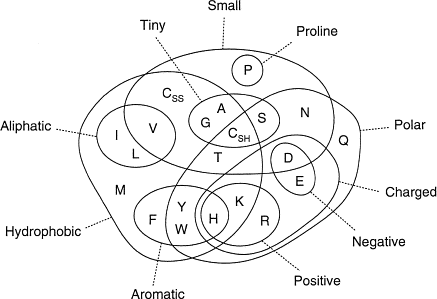
\includegraphics[width=1\linewidth]{img/aa_venn_diagram} \caption{Top ten features ranked according to
\emph{Gini importance}. omes\_apc = OMES contact score with
\protect\hyperlink{abbrev}{APC}, MI\_apc = mutual information score with
\protect\hyperlink{abbrev}{APC}, prior\_L = contact prior based on
protein length as described in methods section
\ref{seq-features-global}, log\_L = logarithm of protein length,
miyasawajernigan1999water = mean pairwise contact potential based on
quasi-chemical potential by Miyazawa \& Jernigan (1999)
{[}\protect\hyperlink{ref-Miyazawa1999a}{91}{]}, rsa\_i amd rsa\_j =
solvent accessibility prediction for residues i and j with NetsurfP
{[}{\textbf{???}}{]}.}\label{fig:rf-feature-importance}
\end{figure}

Many features receive only very low \emph{Gini importance} scores. In
order to reduce the complexity of the model that comprises 225 features,
it is convenient to evaluate model performance on subsets of highly
important features only (see methods section
\ref{rf-feature-selection}). As can be seen in Figure
\ref{rf-performance-feature-selection}, most models trained on subsets
of the feature space perform nearly identical to the model trained on
the complete feature set.






\begin{figure}
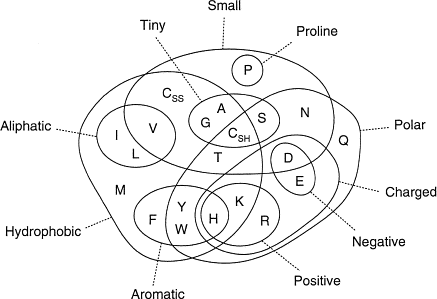
\includegraphics[width=1\linewidth]{img/aa_venn_diagram} \caption{Average precision of
random forest models trained on subsets of sequence derived features.
Subsets of features have been selected as described in methods section
\ref{rf-feature-selection}.}\label{fig:rf-performance-feature-selection}
\end{figure}

The model using the 75 most important features according to \emph{Gini
importance} has been selected for further analysis. Figure
\ref{rf-with-pll-score} compares performance of various models. The
random forest model trained on the 75 most important features (green
line) has a mean precision of 0.33 for the top 5L contacts compared to a
precision of 0.47 for the conventional L2norm + APC contact score based
on pseudo-likelihood optimization (red line). The performance of the two
local statistical contact scores, OMES+APC and MI+APC, which also
constitute the two most important features of the random forest model,
are shown as blue and yellow lines in Figure \ref{rf-with-pll-score}.
The random forest model improves approximately ten percentage points in
precision over both methods.

When analysing performance with respect to alignment size it is clear
that the random forest model outperforms the pseudo-likelihood score for
small alignments. Both, OMES and MI also perform weak on small
alignments, leading to the conclusion that the remaining sequence
derived features are highly relevant in the regimes low data.

In order to evaluate how much the sequence derived features can improve
contact prediction over the coevolutionary contact scores, the
coevolutionary contact score can simply be included as an additional
feature into the Random Forest model.

The model was trained as described in methods section
\ref{rf-with-pll-score} using the additional pseudo-likelihood score
feature. As expected, the pseudo-likelihood score comprises the most
important feature in the model as can be seen in Figure
\ref{fig:feature-importance-rf-with-pll-score}. Furthermore, feature
selection analysis shows that by using only the 26 most important
features improves the model further (see Figure
\ref{fig:feature-selection-rf-with-pll-score}).

Using the default pseudo-likelihood contact score (L2norm + APC) as an
additional coevolutionary feature indeed improves performance (see
Figure \ref{fig:performance-rf-with-pll-score}) over the score without
prior information.













\begin{figure}
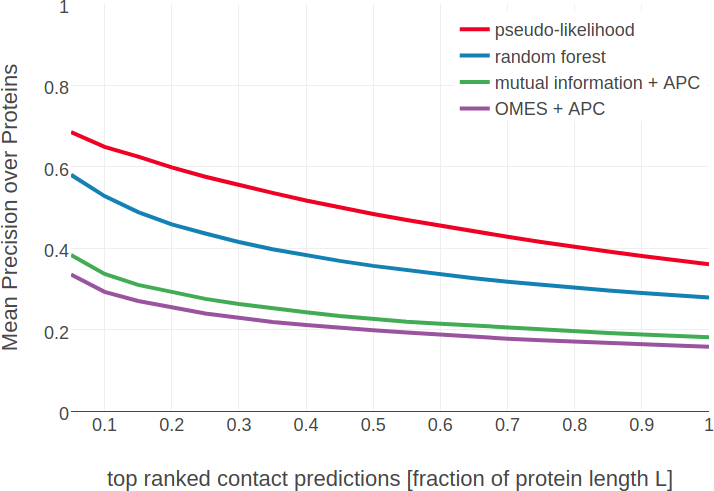
\includegraphics[width=1\linewidth]{img/random_forest_contact_prior/precision_vs_rank_notitle} \caption{Mean Precision for top
ranked contacts on a test set of \textasciitilde{}500 proteins.
\textbf{omes\_fodoraldrich+apc} = OMES score with APC as described in
section \ref{seq-features-pairwise}. \textbf{mi\_pc + APC} = mutual
information with APC as described in section
\ref{seq-features-pairwise}. \textbf{rf\_contact\_prior} = random forest
model using only sequence derived features. \textbf{pLL-L2normapc-RF} =
random forest model using sequence derived features and
pseudo-likelihood contact score (L2norm + APC).
\textbf{ccmpred-pll-centerv+apc} = conventional pseudo-likelihood
contact score (L2norm + APC)}\label{fig:performance-rf-with-pll-score}
\end{figure}

Especially for small alignments, the random forest model makes better
predictions than the coevolutionary method. This finding is expected, as
it is well known that models trained on simple sequence features perform
almost independent of alignment size. {[}{\textbf{???}},
\textbf{???}{]}. In contrast, the improvement on large alignments is
small, as the gain from simple sequence features compared to the much
more powerful coevolution signals is neglectable.



\begin{figure}
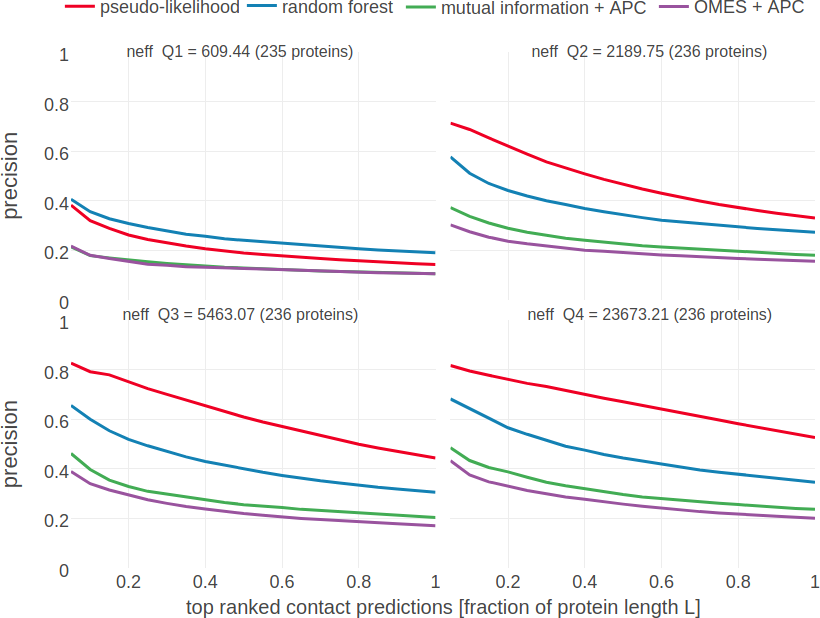
\includegraphics[width=1\linewidth]{img/random_forest_contact_prior/precision_vs_rank_facetted_by_neff_notitle} \caption{blabla neff}\label{fig:performance-neff-rf-with-pll-score}
\end{figure}

\chapter{Methods}\label{methods}

all you need to know

\section{Dataset}\label{dataset}

A protein dataset has been constructed from the CATH (v4.1)
{[}\protect\hyperlink{ref-Sillitoe2015}{92}{]} database for
classification of protein domains. All CATH domains from classes
1(mainly \(\alpha\)), 2(mainly \(\beta\)), 3(\(\alpha+\beta\)) have been
selected and filtered for internal redundancy at the sequence level
using the \texttt{pdbfilter} script from the
HH-suite{[}\protect\hyperlink{ref-Remmert2012}{73}{]} with an E-value
cutoff=0.1. The dataset has been split into ten subsets aiming at the
best possible balance between CATH classes 1,2,3 in the subsets. All
domains from a given CATH topology (=fold) go into the same subsets, so
that any two subsets are non-redundant at the fold level. Some
overrepresented folds (e.g.~Rossman Fold) have been subsampled ensuring
that in every subset each class contains at max 50\% domains of the same
fold. Consequently, a fold is not allowed to dominate a subset or even a
class in a subset. In total there are 6741 domains in the dataset.

Multiple sequence alignments were built from the CATH domain sequences
(\href{http://www.cathdb.info/version/current/domain/3cdjA03/sequence}{COMBS})
using HHblits {[}\protect\hyperlink{ref-Remmert2012}{73}{]} with
parameters to maximize the detection of homologous sequences:

\texttt{hhblits\ -maxfilt\ 100000\ -realign\_max\ 100000\ -B\ 100000\ -Z\ 100000\ -n\ 5\ -e\ 0.1\ -all}
\texttt{hhfilter\ -id\ 90\ -neff\ 15\ -qsc\ -30}

The COMBS sequences are derived from the SEQRES records of the PDB file
and sometimes contain extra residues that are not resolved in the
structure. Therefore, residues in PDB files have been renumbered to
match the COMBS sequences. The process of renumbering residues in PDB
files yielded ambigious solutions for 293 proteins, that were removed
from the dataset. Another filtering step was applied to remove 80
proteins that do not hold the following properties:

\begin{itemize}
\tightlist
\item
  more than 10 sequences in the multiple sequence alignment (\(N>10\))
\item
  protein length between 30 and 600 residues (\(30 \leq L \leq 600\))
\item
  less than 80\% gaps in the multiple sequence alignment (percent gaps
  \textless{} 0.8)
\item
  at least one residue-pair in contact at \(C_\beta < 8\AA\) and minimum
  sequence separation of 6 positions
\end{itemize}

The final dataset is comprised of \textbf{6368} proteins with almost
evenly distributed CATH classes over the ten subsets (Figure
\ref{fig:dataset-cath-topologies}).





\begin{figure}
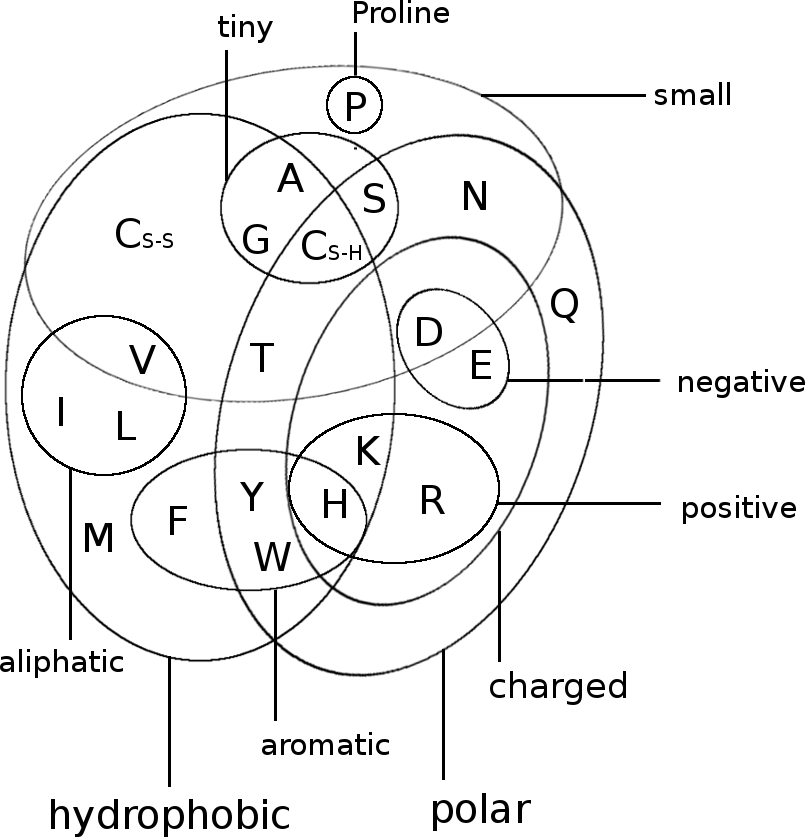
\includegraphics[width=1\linewidth]{img/amino_acid_physico_chemical_properties_venn_diagramm} \caption{Distribution of CATH classes
(1=mainly \(\alpha\), 2=mainly \(\beta\), 3=\(\alpha-\beta\)) in the
dataset and the ten subsets. }\label{fig:dataset-cath-topologies}
\end{figure}

\section{Optimizing
Pseudo-Likelihood}\label{optimizing-pseudo-likelihood}

Dr Stefan Seemayer has reimplementated the open-source software CCMpred
{[}\protect\hyperlink{ref-Seemayer2014}{59}{]} in Python. Based on a
fork of his private github repository I continued development and
extended the software, which is now called CCMpredPy. It will soon be
available at \url{https://github.com/soedinglab/CCMpredPy}. All
computations in this thesis are performed with CCMpredPy unless stated
otherwise.

\subsection{Pseudo-Likelihood Objective Function and its
Gradients}\label{pseudo-likelihood-objective-function-and-its-gradients}

CCMpred optimizes the regularized negative pseudo-log-likelihood using
conjugate gradients optimizer.

The negative pseudo-log-likelihood, abbreviated \(\mathcal{npll}\), is
defined as:

\begin{equation}
  \mathcal{npll}(\mathbf{X} | \v,\w) =   - \sum_{n=1}^N \sum_{i=1}^L  \left(  v_i(x_i^{(n)}) + \sum_{\substack{j=1 \\ j \neq i}}^L w_{ij}(x_i^{(n)}, x_j^{(n)})  - \log Z_i^{(n)} \right)
\end{equation}

The normalization term \(Z_i\) sums over all assignments to one position
\(i\) in sequence:

\begin{equation}
  Z_i^{(n)} = \sum_{a=1}^{20} \exp \left( v_i(a) + \sum_{\substack{j=1 \\ j \neq i}}^L w_{ij}(a, x_j^{(n)}) \right)
\end{equation}

\subsection{Differences between CCMpred and
CCMpredpy}\label{diff-ccmpred-ccmpredpy}

CCMpredPy differs from CCMpred
{[}\protect\hyperlink{ref-Seemayer2014}{59}{]} which is available at
\url{https://github.com/soedinglab/CCMpred} in several details:

\begin{itemize}
\tightlist
\item
  Initialization of potentials \(\v\) and \(\w\)

  \begin{itemize}
  \tightlist
  \item
    CCMpred initializes single potentials
    \(\v_i(a) = \log f_i(a) - \log f_i(a= "-")\) with \(f_i(a)\) being
    the frequency of amino acid a at position i and \(a="-"\)
    representing a gap. A single pseudo-count has been added before
    computing the frequencies. Pair potentials \(\w\) are intialized at
    0.
  \item
    CCMpredPy initializes single potentials \(\v\) with the
    \protect\hyperlink{abbrev}{ML} estimate of single potentials (see
    section \ref{regularization}) using amino acid frequencies computed
    as described in section \ref{amino-acid-frequencies}. Pair
    potentials \(\w\) are initialized at 0.
  \end{itemize}
\item
  Regularization

  \begin{itemize}
  \tightlist
  \item
    CCMpred uses a Gaussian regularization prior centered at zero for
    both single and pair potentials. The regularization coefficient for
    single potentials \(\lambda_v = 0.01\) and for pair potentials
    \(\lambda_w = 0.2 * (L-1)\) with \(L\) being protein length.
  \item
    CCMpredPy uses a Gaussian regularization prior centered at zero for
    the pair potentials. For the single potentials the Gaussian
    regularization prior is centered at the
    \protect\hyperlink{abbrev}{ML} estimate of single potentials (see
    section \ref{regularization}) using amino acid frequencies computed
    as described in section \ref{amino-acid-frequencies}. The
    regularization coefficient for single potentials \(\lambda_v = 10\)
    and for pair potentials \(\lambda_w = 0.2 * (L-1)\) with \(L\) being
    protein length.
  \end{itemize}
\end{itemize}

Default settings for CCMpredPy have been chosen to best reproduce
CCMpred results. A benchmark over a subset of approximately 3000
proteins confirms that performance measured as
\protect\hyperlink{abbrev}{PPV} for both methods is almost identical
(see Figure \ref{fig:cmmpredvanilla-vs-ccmpredpy}).









\begin{figure}
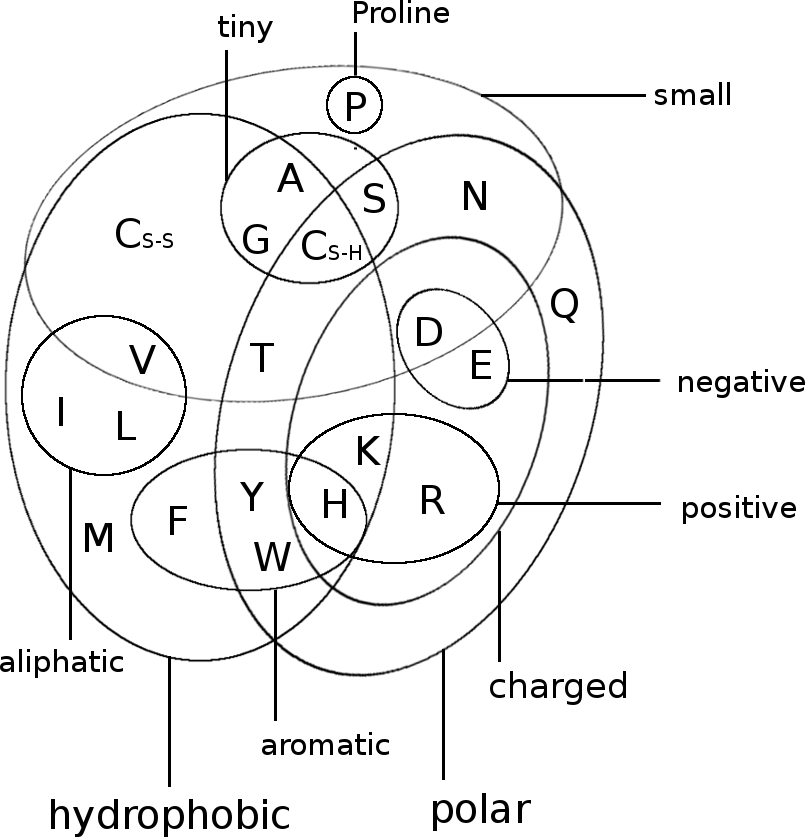
\includegraphics[width=1\linewidth]{img/amino_acid_physico_chemical_properties_venn_diagramm} \caption{Benchmark for CCMpred and
CCMpredPy on a dataset of 3124 proteins. ccmpred-vanilla+apc: CCMpred
{[}\protect\hyperlink{ref-Seemayer2014}{59}{]} with
\protect\hyperlink{abbrev}{APC}. ccmpred-pll-centerv+apc: CCMpredPy with
\protect\hyperlink{abbrev}{APC}. Specific flags that have been used to
run both methods are described in detail in the text (see section
\ref{diff-ccmpred-ccmpredpy}).}\label{fig:cmmpredvanilla-vs-ccmpredpy}
\end{figure}

The benchmark in Figure \ref{fig:cmmpredvanilla-vs-ccmpredpy} as well as
all contacts predicted with CCMpred and CCMPredPy (using
pseudo-likelihood) in my thesis have been computed using the following
flags:

Flags used with CCMpredPy (using pseudo-likelihood objective function):

\begin{verbatim}
--maxit 250                       # Compute a maximum of MAXIT operations
--center-v                        # Use a Gaussian prior for single potentials centered at ML estimate v*
--reg-l2-lambda-single 10         # regularization coefficient for single potentials
--reg-l2-lambda-pair-factor 0.2   # regularization coefficient for pairwise potentials computed as reg-l2-lambda-pair-factor * (L-1)
--pc-uniform                      # use uniform pseudocounts (1/21 for 20 amino acids + 1 gap state) 
--pc-count 1                      # defining pseudo count admixture coefficient rho = pc-count/( pc-count+ Neff)
--epsilon 1e-5                    # convergence criterion for minimum decrease in the last K iterations
--ofn-pll                         # using pseudo-likelihood as objective function
--alg-cg                          # using conjugate gradient to optimize objective function
\end{verbatim}

Flags used with CCMpred:

\begin{verbatim}
-n 250    # NUMITER:  Compute a maximum of NUMITER operations
-l 0.2    # LFACTOR:  Set pairwise regularization coefficients to LFACTOR * (L-1) 
-w 0.8    # IDTHRES:  Set sequence reweighting identity threshold to IDTHRES
-e 1e-5   # EPSILON:  Set convergence criterion for minimum decrease in the last K iterations to EPSILON
\end{verbatim}

\subsection{Sequence Reweighting}\label{seq-reweighting}

As discussed in section \ref{challenges}, sequences in a
\protect\hyperlink{abbrev}{MSA} do not represent independent draws from
a probabilistic model. To reduce the effects of overrepresented
sequences, typically a simple weighting strategy is applied that assigns
a weight to each sequence that is the inverse of the number of similar
sequences according to an identity threshold
{[}\protect\hyperlink{ref-Stein2015a}{58}{]}. It has been found that
reweighting improves contact prediction performance
{[}\protect\hyperlink{ref-Jones2012}{44},\protect\hyperlink{ref-Morcos2011}{53},\protect\hyperlink{ref-Buslje2009}{70}{]}
significantly but results are robust against the choice of the identity
threshold in a range between 0.7 and 0.9
{[}\protect\hyperlink{ref-Morcos2011}{53}{]}. We chose an identity
threshold of 0.8.

Every sequence \(x_n\) of length \(L\) in an alignment with \(N\)
sequences has an associated weight \(w_n = 1/m_n\), where \(m_n\)
represents the number of similar sequences:

\begin{equation} 
  w_n = \frac{1}{m_n}, m_n = \sum_{m=1}^N I \left( ID(x_n, x_m) \geq 0.8 \right) \\
  ID(x_n, x_m)=\frac{1}{L} \sum_{i=1}^L I(x_n^i = x_m^i)
  \label{eq:seqweight}
\end{equation}

The number of effective sequences \(\mathbf{\neff}\) of an alignment is
then the number of sequence clusters computed as:

\begin{equation} 
  \neff = \sum_{n=1}^N w_n
  \label{eq:neff}
\end{equation}

TODO: Plot Performance for Seq weighting

\subsection{Computing Amino Acid
Frequencies}\label{amino-acid-frequencies}

Single and pairwise amino acid frequencies are computed from the
alignment by weighting amino acid counts (see section
\ref{seq-reweighting}) and adding pseudocounts for numerical stability.

Let \(a,b \in \{1,\ldots,20\}\) be amino acids,
\(q(x_i=a), q(x_i=a, x_j=b)\) and \(q_0(x_i=a), q_0(x_i=a,x_j=b)\) be
the empirical single and pair frequencies with and without pseudocounts,
respectively. We define

\begin{align}
    q(x_i \eq a) :=& (1-\tau) \;  q_0(x_i \eq a) + \tau \tilde{q}(x_i\eq a) \\
    q(x_i \eq a, x_j \eq b) :=& (1-\tau)^2  \; [ q_0(x_i \eq a, x_j \eq b) - q_0(x_i \eq a)  q_0(x_j \eq b) ] + \\
                            & q(x_i \eq a) \; q(x_j \eq b) 
\label{eq:pseudocounts}
\end{align}

with \(\tilde{q}(x_i \eq a) := f(a)\) being background amino acid
frequencies and \(\tau \in [0,1]\) is a pseudocount admixture
coefficient, which is a function of the diversity of the multiple
sequence alignment:

\begin{equation}
    \tau = \frac{N_\mathrm{pc}}{(N_\mathrm{eff} + N_\mathrm{pc})}
\label{eq:tau}
\end{equation}

where \(N_{pc} > 0\).

The formula for \(q(x_i \eq a, x_j \eq b)\) in the second line in eq
\eqref{eq:pseudocounts} was chosen such that for \(\tau \eq0\) we obtain
\(q(x_i \eq a, x_j \eq b) = q_0(x_i \eq a, x_j \eq b)\), and furthermore
\(q(x_i \eq a, x_j \eq b) = q(x_i \eq a) q(x_j \eq b)\) exactly if
\(q_0(x_i \eq a, x_j \eq b) = q_0(x_i \eq a) q_0(x_j \eq b)\).

\subsection{Regularization}\label{regularization}

As the model is overparameterized, regularization is an alternative
solution compared to choosing a gauge. Furthermore it helps preventing
overfitting.

L2-regularization which corresponds to using a Gaussian prior, has
proven to work better than L1 regularization {[}{\textbf{???}}{]}.

\begin{equation}
  R(\v, \w) = \mathcal{N}(\v |  \vec{0}, \lambda_v \I^{-1})  + \mathcal{N}(\w | \vec{0}, \lambda_w \I^{-1}) 
\end{equation}

\begin{align}
 \mathcal{N}(\v |  \vec{0}, \lambda_v \I^{-1})   &= \lambda_v ||\v||_2^2 \\
                                                &= \frac{\lambda_v}{2} \sum_{i=1}^L \sum_{a=1}^{20}  \via^2
\end{align}

\begin{align}
\mathcal{N}(\w | \vec{0}, \lambda_w \I^{-1}) &= \lambda_w ||\w||_2^2 \\
                                            &= \frac{\lambda_w}{2} \sum_{i=1}^L \sum_{\substack{j=1 \\ i \neq j}}^L  \sum_{a,b=1}^{20} \wijab^2
\end{align}

However, it makes sense to use a Gaussian prior for single emission
potentials that is centered at the \protect\hyperlink{abbrev}{ML}
estimate of the single potentials. Consider, \ldots{}..

\begin{align}
 \mathcal{N}(\v |  \v^{*}, \lambda_v \I^{-1}) &= \lambda_v ||\v - \v^{*}||_2^2 \\
                                               &= \frac{\lambda_v}{2} \sum_{i=1}^L \sum_{a=1}^{20}  (\via - \via^{*})^2   
\end{align}

\begin{equation}
  \via^* = \log q(x_i=a) - \frac{1}{20} \sum_{a'=1}^{20} \log q(x_i=a')
\end{equation}

\section{Analysis of Coupling
Matrices}\label{analysis-of-coupling-matrices}

\subsection{Correlation of Couplings with Contact
Class}\label{method-coupling-correlation}

Approximately 100000 residue pairs have been filtered for contacts and
non-contacts respectively according to the following criteria:

\begin{itemize}
\tightlist
\item
  consider only residue pairs separated by at least 10 positions in
  sequence
\item
  minimal diversity (\(=\frac{\sqrt{N}}{L}\)) of alignment = 0.3
\item
  minimal number of non-gapped sequences = 1000
\item
  \(\Cb\) distance threshold for contact: \(<8\AA\)
\item
  \(\Cb\) distance threshold for noncontact: \(>25\AA\)
\end{itemize}

\subsection{Coupling Distribution Plots}\label{method-coupling-profile}

For one-dimensional coupling distribution plots the residue pairs and
respective pseudo-log-likelihood coupling values \(\wijab\) have been
selected as follows:

\begin{itemize}
\tightlist
\item
  consider only residue pairs separated by at least 10 positions in
  sequence
\item
  discard residues that have more than 30\% gaps in the alignment
\item
  discard residue pairs that have insufficient evidence in the
  alignment: \(N_{ij} \cdot q_i(a) \cdot q_j(b) < 100\) with:

  \begin{itemize}
  \tightlist
  \item
    \(N_{ij}\) is the number of sequences with neither a gap at position
    i nor at position j
  \item
    \(q_i(a)\) and \(q_j(b)\) are the frequencies of amino acids a and b
    at positions i and j (computed as described in section
    \ref{amino-acid-frequencies})
  \end{itemize}
\end{itemize}

The same criteria have been applied for selecting couplings for the
two-dimensional distribution plots with the difference that evidence for
a single coupling term has to be
\(N_{ij} \cdot q_i(a) \cdot q_j(b) < 80.\)

\section{Optimizing the
Full-Likelihood}\label{methods-optimizing-full-likelihood}

Given the likelihood gradient estimate utilizing contrastive divergence,
the full likelihood can now be minimized using a gradient descent
optimization algorithm. Second order optimization algorithms that make
use of the (approximate) partial second derivates cannot be applied
here, as the computation of the Hessian is too complex.

Gradient descent algorithms in general minimize an objective function by
iteratively updating the function parameters in the opposite direction
of the gradient of the objective function with respect to the
parameters. Stochastic gradient descent is a variant thereof that uses
only a subsample of the data at each step of the optimization procedure
to estimate the gradient. Consequently, the gradient estimates are noisy
resulting in parameter updates with high variance and strong
fluctuations of the objective function. These fluctuation enable
stochastic gradient descent to escape local minima but also complicate
finding the exact minimum of the objective function. By slowly
decreasing the step size of the parameter updates at every iteration,
stochastic gradient descent most likely will converge to the global
minimum for convex objective functions
{[}{\textbf{???}},{\textbf{??}}{]}.

However, choosing an optimal learning rate for parameter updates as well
as an appropriate learning rate decay offers a challenge and needs
manual tuning. The following sections describe the hyperparameter
optimization of two stochastic gradient descent optimization algorithms:
simple stochastic gradient descent and ADAM
{[}\protect\hyperlink{ref-Kingma2014}{93}{]}. The performance for tested
parameter settings is evaluated on a benchmark set of \textasciitilde{}
500 proteins, that is a subset of the data set described in methods
section \ref{dataset}. The reference method for all new developed scores
is the pseudo-likelihood method that uses the corrected L2norm as a
final contact score as explained in section
\ref{post-processing-heuristics}. Pseudo-likelihood couplings are
computed with the tool CCMpredPy that is introduced in methods section
\ref{diff-ccmpred-ccmpredpy}. Contact scores for the methods under
developments are computed using the corrected L2norm of the couplings,
just as for the pseudo-likelihood method.

\subsection{Hyperparameter Optimization for Stochastic Gradient
Descent}\label{hyperparameter-optimization-for-stochastic-gradient-descent}

Stochastic gradient descent updates the coupling parameters \(\w\) using
the approximate gradient to the log likelihood
\(\nabla_w \LLreg(\v,\w)\) obtained with contrastive divergence and a
learning rate \(\alpha\) according to

\begin{equation}
  \w_{t+1} = \w_t - \alpha \cdot \nabla_w \LLreg(\v,\w) \; .
\end{equation}

In order to get a first intuition of the optimization problem, I used
\(\alpha \in \{1\mathrm{e}{-4}, 5\mathrm{e}{-4}, 1\mathrm{e}{-3}, 5\mathrm{e}{-3}\}\)
and a standard learning rate schedule,

\begin{equation}
  \alpha  = \frac{\alpha_0}{1 + \gamma \cdot t} \; ,
\end{equation}

with \(\gamma=0.1\) being the decay rate and \(t\) the current iteration
{[}{\textbf{???}}{]}. It is not feasible to compute the function value
at each iteration in order to decide when the optimization has
converged. Therefore the optimization will stop whenever the gradient
norm changes less than a small \(\epsilon=1\mathrm{e}{-8}\) or when 5000
iterations are reached.

Figure \ref{fig:performance-cd-alphaopt} shows the benchmark for the
optimizations with the four different learning rates. In general, the
top ranked contacts are predicted with equal accuracy as the reference
method ({``ccmpred-pll-centerv+apc''}) when using small learning rates
\(\alpha \in \{1\mathrm{e}{-4}, 5\mathrm{e}{-4}, 1\mathrm{e}{-3} \}\).
Predictions for lower ranked contacts (top \(0.6-L\) predictions) are
less accurate. Using a high learning rate \(5\mathrm{e}{-3}\) yields
much less accurate predictions. When evaluating the methods with respect
to alignment size (see Figure \ref{fig:performance-cd-alphaopt-neff}) it
becomes clear that a high learning rate of \(5\mathrm{e}{-3}\) does only
not work well for proteins with large alignments. The magnitude of the
gradient depends on the size of the alignment because the gradient is
computed as a difference of amino acid counts. Therefore proteins with
large alignments will generally have larger gradients than proteins with
small alignments. When analysing individual proteins with large
alignments it becomes clear that choosing a learning rate that is too
large causes the optimization to diverge. Furthermore, when using a
small learning rate, most of the optimizations did not converge but
reached the maximum number of 5000 iterations.












\begin{figure}

{\centering 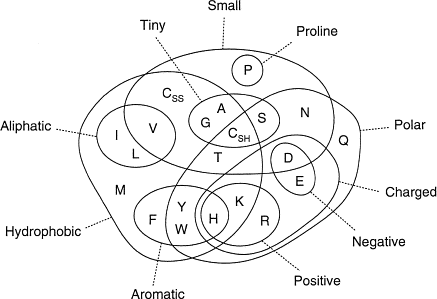
\includegraphics[width=0.9\linewidth]{img/aa_venn_diagram} 

}

\caption{Mean precision for top ranked
contact predictions over \textasciitilde{}500 proteins.
{ccmpred-pll-centerv+apc}: L2norm + APC score for pseudo-likelihood
couplings. The other methods derive contact scores as the L2norm + APC
for couplings computed with contrastive divergence using stochastic
gradient descent and different learning rates: {cd\_alpha\_1e-4+apc}:
learning rate \(1\mathrm{e}{-4}\). {cd\_alpha\_5e-4+apc}: learning rate
\(5\mathrm{e}{-4}\). {cd\_alpha\_1e-3+apc}: learning rate
\(1\mathrm{e}{-3}\). {cd\_alpha\_5e-3+apc}: learning rate
\(5\mathrm{e}{-3}\).}\label{fig:performance-cd-alphaopt}
\end{figure}














\begin{figure}

{\centering 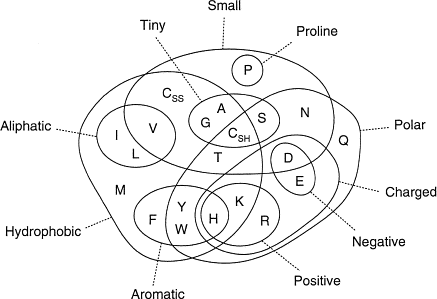
\includegraphics[width=0.9\linewidth]{img/aa_venn_diagram} 

}

\caption{Mean precision for top ranked
contact predictions over \textasciitilde{}500 proteins splitted into
four equally sized subsets according to
\protect\hyperlink{abbrev}{Neff}. Subsets are defined according to
quantiles of \protect\hyperlink{abbrev}{Neff} values. Upper left: Subset
of proteins with \protect\hyperlink{abbrev}{Neff} \textless{} Q1. Upper
right: Subset of proteins with Q1 \textless{}=
\protect\hyperlink{abbrev}{Neff} \textless{} Q2. Lower left: Subset of
proteins with Q2 \textless{}= \protect\hyperlink{abbrev}{Neff}
\textless{} Q3. Lower right: Subset of proteins with Q3 \textless{}=
\protect\hyperlink{abbrev}{Neff} \textless{} Q4. Methods are the same as
in Figure \ref{fig:performance-cd-alphaopt}.}\label{fig:performance-cd-alphaopt-neff}
\end{figure}

\section{Bayesian Model for Residue-Resdiue Contact
Prediction}\label{bayesian-model-for-residue-resdiue-contact-prediction}

\subsection{Efficiently Computing the negative Hessian of the
regularized log-likelihood}\label{neg-Hessian-computation}

Surprisingly, the elements of the Hessian at the mode \(\w^*\) are easy
to compute. Let \(i,j,k,l \in \{1,\ldots,L\}\) be columns in the
\protect\hyperlink{abbrev}{MSA} and let
\(a, b, c, d \in \{1,\ldots,20\}\) represent amino acids.

The partial derivative \(\partial / \partial \w_{klcd}\) of the second
term in the gradient of the couplings in eq.
\eqref{eq:gradient-LLreg-pair} is

\begin{eqnarray}
    \frac{\partial^2 \LLreg(\v^*,\w)}{\partial \wklcd \, \partial \wijab } 
    &=&  - \sum_{n=1}^{N} \, \sum_{\mathbf{y} \in \Sn} \frac{\partial \left( \frac{\exp \left( \sum_{i=1}^L v_i(y_i) + \sum_{1 \le i < j \le L}^L w_{ij}(y_i,y_j) \right) }{Z_n(\v,\w)} \right)}{\partial \wklcd}   I(y_i \eq a, y_j \eq b) \\
    &&- \lambda_w \delta_{ijab,klcd} \,,
\end{eqnarray}

where \(\delta_{ijab,klcd} = I(ijab=klcd)\) is the Kronecker delta.
Applying the product rule, we find

\begin{eqnarray}
    \frac{\partial^2 \LLreg(\v^*,\w)}{\partial \wklcd \, \partial \wijab  } 
    &=&  - \sum_{n=1}^{N} \, \sum_{\mathbf{y} \in \Sn} \frac{\exp \left(\sum_{i=1}^L v_i(y_i) + \sum_{1 \le i < j \le L}^L w_{ij}(y_i,y_j)  \right)}{Z_n(\v,\w)}  I(y_i \eq a, y_j \eq b) \\
    & \times & \left[ \frac{\partial}{\partial \wklcd} \left( \sum_{i=1}^L v_i(y_i) + \sum_{1 \le i < j \le L}  w_{ij}(y_i,y_j)  \right) 
                  - \frac{1}{Z_n(\v,\w)} \frac{\partial  Z_n(\v,\w) }{\partial\wklcd} \right] \\
    &-& \lambda_w \delta_{ijab,klcd} \\
    \frac{\partial^2 \LLreg(\v^*,\w)}{\partial \wklcd \, \partial \wijab  } 
    &=&  - \sum_{n=1}^{N} \, \sum_{\mathbf{y} \in \Sn} \frac{\exp \left(\sum_{i=1}^L v_i(y_i) + \sum_{1 \le i < j \le L}^L w_{ij}(y_i,y_j)  \right)}{Z_n(\v,\w)}  I(y_i \eq a, y_j \eq b) \\
    & \times & \left[ I(y_k \eq c, y_l \eq d) - \frac{\partial}{\partial \wklcd} \log Z_n(\v,\w) \right] \\
    &-& \lambda_w \delta_{ijab,klcd} \,.
\end{eqnarray}

We simplify this expression using

\begin{equation}
    p(\mathbf{y} | \v,\w) = \frac{\exp \left( \sum_{i=1}^L v_i(y_i) + \sum_{1 \le i < j \le L} w_{ij}(y_i,y_j) \right)}{Z_n(\v,\w)}  ,
\end{equation}

yielding

\begin{eqnarray}
    \frac{\partial^2 \LLreg(\v^*,\w)}{\partial \wklcd \, \partial \wijab} 
    &=&  -  \sum_{n=1}^{N} \, \sum_{\mathbf{y} \in \Sn} p(\mathbf{y} | \v,\w) \, I(y_i \eq a, y_j \eq b, y_k \eq c, y_l \eq d)  \\
    &+& \sum_{n=1}^{N} \, \sum_{\mathbf{y} \in \mathcal{S}_n} p(\mathbf{y} | \v,\w) \, I(y_i \eq a, y_j \eq b ) \sum_{\mathbf{y} \in \Sn} p(\mathbf{y} | \v,\w)  I(y_k \eq c, y_l \eq d ) \\
    &-& \lambda_w \delta_{ijab,klcd} \,.
\end{eqnarray}

If \(\X\) does not contain too many gaps, this expression can be
approximated by

\begin{eqnarray}
    \frac{\partial^2 \LLreg(\v^*,\w)}{\partial \wklcd \, \partial \wijab  } 
    &=& - N_{ijkl} \: p(x_i \eq a, x_j \eq b, x_k \eq c, x_l \eq d | \v,\w)  \nonumber \\
    && +  N_{ijkl} \: p(x_i \eq a, x_j \eq b | \v,\w) \, p(x_k \eq c, x_l \eq d | \v,\w) - \lambda_w \delta_{ijab,klcd} \,,
\end{eqnarray}

where \(N_{ijkl}\) is the number of sequences that have a residue in
\(i\), \(j\), \(k\) and \(l\).

Looking at three cases separately:

\begin{itemize}
\tightlist
\item
  case 1: \((k,l) = (i,j)\) and \((c,d) = (a,b)\)
\item
  case 2: \((k,l) = (i,j)\) and \((c,d) \ne (a,b)\)
\item
  case 3: \((k,l) \ne (i,j)\) and \((c,d) \ne (a,b)\),
\end{itemize}

the elements of \(\H\), which are the negative second partial
derivatives of \(\LLreg(\v^*,\w)\) with respect to the components of
\(\w\), are

\begin{eqnarray}
    \mathrm{case~1:} (\H)_{ijab, ijab}  
    &=&  N_{ij} \, p(x_i \eq a, x_j \eq b| \v^*,\w^*) \, ( 1 - p(x_i \eq a, x_j \eq b| \v^*,\w^*) \,) \\
    &&   + \lambda_w \\
    \mathrm{case~2:} (\H)_{ijcd, ijab}  
    &=&  - N_{ij} \, p(x_i \eq a, x_j \eq b |\v^*,\w^*) \, p(x_i \eq c, x_j \eq d |\v^*,\w^*) \\
    \mathrm{case~3:} (\H)_{klcd, ijab}  
    &=&   N_{ijkl} \, p(x_i \eq a, x_j \eq b, x_k \eq c, x_l \eq d  | \v^*,\w^*) \nonumber \\
    &&    - N_{ijkl} \, p(x_i \eq a, x_j \eq b | \v^*,\w^*)\, p(x_k \eq c, x_l \eq d | \v^*,\w^*) \,.
\label{eq:Hw-offdiag}
\end{eqnarray}

We know from eq. \eqref{eq:gradient-LLreg-approx} that at the mode
\(\w^*\) the model probabilities match the empirical frequencies up to a
small regularization term,

\begin{equation}
    p(x_i \eq a, x_j \eq b | \v^*,\w^*) = q(x_i \eq a, x_j \eq b) - \frac{\lambda_w}{N_{ij}}  \wijab^* \,,
\end{equation}

and therefore the negative Hessian elements in cases 1 and 2 can be
expressed as

\begin{align}
   (\H)_{ijab, ijab} =& N_{ij} \left( q(x_i \eq a, x_j \eq b)  - \frac{\lambda_w}{N_{ij}} \wijab^* \right) \left( 1 - q(x_i \eq a, x_j \eq b) +\frac{\lambda_w}{N_{ij}} \wijab^* \right) \\
   & + \lambda_w \\
   (\H)_{ijcd, ijab} =& -N_{ij} \left(\,q(x_i \eq a, x_j \eq b)  - \frac{\lambda_w}{N_{ij}} \wijab^* \right) \left( q(x_i \eq c, x_j \eq d) -\frac{\lambda_w}{N_{ij}} \wijcd^* \right) .
\label{eq:Hw-diag}
\end{align}

In order to write the previous eq. \eqref{eq:Hw-diag} in matrix form, the
\emph{regularised} empirical frequencies \(\qij\) will be defined as

\begin{equation}
    (\qij)_{ab} = q'_{ijab} := q(x_i \eq a, x_j \eq b) - \lambda_w  \wijab^* / N_{ij} \,,
\end{equation}

and the \(400 \times 400\) diagonal matrix \(\Qij\) will be defined as

\begin{equation}
    \Qij := \text{diag}(\qij) \; .
\end{equation}

Now eq. \eqref{eq:Hw-diag} can be written in matrix form

\begin{equation}
     \H_{ij} = N_{ij} \left( \Qij -  \qij \qij^{\mathrm{T}} \right)  + \lambda_w \I \; .
\label{eq:mat-Hij}
\end{equation}

\subsection{\texorpdfstring{Efficiently Computing the Inverse of Matrix
\(\Lijk\)}{Efficiently Computing the Inverse of Matrix \textbackslash{}Lijk}}\label{inv-lambda-ij-k}

It is possible to efficiently invert the matrix
\(\Lijk = \H_{ij} - \lambda_w \I + \Lambda_k\), that is introduced in
\ref{coupling-prior} where \(\H_{ij}\) is the \(400 \times 400\)
diagonal block submatrix \((\H_{ij})_{ab,cd} := (\H)_{ijab,ijcd}\) and
\(\Lambda_k\) is an invertible diagonal precision matrix that is
introduced in section \ref{modeling-dep-of-wij}.

Equation \eqref{eq:mat-Hij} can be used to write \(\Lijk\) in matrix form
as

\begin{equation}
     \Lijk = \H_{ij} - \lambda_w \I + \Lk = N_{ij} \Qij- N_{ij} \qij \qij^{\mathrm{T}} + \Lk \,.
\label{eq:mat-Lijk}
\end{equation}

Owing to eqs. \eqref{eq:normalized-emp-freq} and \eqref{eq:zero-sum-wij},
\(\sum_{a,b=1}^{20} q'_{ijab} = 1\). The previous equation
\eqref{eq:mat-Lijk} facilitates the calculation of the inverse of this
matrix using the \emph{Woodbury identity} for matrices

\begin{equation}
    (\mathbf{A} + \mathbf{B} \mathbf{D}^{-1} \mathbf{C})^{-1} = \mathbf{A}^{-1} - \mathbf{A}^{-1} \mathbf{B} (\mathbf{D} + \mathbf{C} \mathbf{A}^{-1} \mathbf{B}) ^{-1} \mathbf{C} \mathbf{A}^{-1} \;. 
\end{equation}

by setting

\begin{align}
  \mathbf{A} &= N_{ij} \Qij + \Lk \\
  \mathbf{B} &= \qij \\
  \mathbf{C} &= \qij^\mathrm{T} \\
  \mathbf{D} &=- N_{ij}^{-1} \\
\end{align}

\begin{align}
      \left( \H_{ij} - \lambda_w \I + \Lk \right)^{-1} & = \mathbf{A}^{-1} - \mathbf{A}^{-1} \qij  \left( -N_{ij}^{-1}  + \qij^\mathrm{T} \mathbf{A}^{-1} \qij \right)^{-1}  \qij^\mathrm{T} \mathbf{A}^{-1} \\
     & = \mathbf{A}^{-1} + \frac{ (\mathbf{A}^{-1} \qij) (\mathbf{A}^{-1} \qij)^{\mathrm{T}} }{ N_{ij}^{-1} - \qij^\mathrm{T} \mathbf{A}^{-1} \qij} \,.
\label{eq:fast-inverse-mat-Lijk}
\end{align}

Note that \(\mathbf{A}\) is diagonal as \(\Qij\) and \(\Lk\) are
diagonal matrices:
\(\mathbf{A} = \text{diag}(N_{ij} q'_{ijab} + (\Lk)_{ab,ab})\).
Moreover, \(\mathbf{A}\) has only positive diagonal elements, because
\(\Lk\) is invertible and has only positive diagonal elements and
because \(q'_{ijab} = p(x_i \eq a, x_j \eq b | \v^*,\w^*) \ge 0\).

Therefore \(\mathbf{A}\) is invertible:
\(\mathbf{A}^{-1} = \text{diag}(N_{ij} q'_{ijab} + (\Lk)_{ab,ab} )^{-1}\).

Because \(\sum_{a,b=1}^{20} q'_{ijab} = 1\), the denominator of the
second term is

\begin{equation}
    N_{ij}^{-1} - \sum_{a,b=1}^{20}  \frac{{q'}_{ijab}^2}{N_{ij} q'_{ijab} + {(\Lk)}_{ab,ab} } > N_{ij}^{-1} - \sum_{a,b=1}^{20} \frac{{q'}^2_{ijab}}{N_{ij} q'_{ijab}} = 0
\end{equation}

and therefore the inverse of \(\Lijk\) in eq.
\eqref{eq:fast-inverse-mat-Lijk} is well defined.

The log determinant of \(\Lijk\) is necessary to compute the ratio of
Gaussians (see equation \eqref{eq:p-X-r-final}) and can be computed using
the matrix determinant lemma:

\begin{equation}
  \det(\mathbf{A} + \mathbf{uv}^\mathrm{T}) = (1+\mathbf{v}^\mathrm{T} \mathbf{A}^{-1} \mathbf{u}) \det(\mathbf{A})
\end{equation}

Setting \(\mathbf{A} = N_{ij} \Qij + \Lk\) and \(\v = \qij\) and
\(\mathbf{u} = - N_{ij} \qij\) yields

\begin{equation}
  \det(\Lijk ) = \det(\H_{ij} - \lambda_w \I + \Lk) = (1 - N_{ij}\qij^\mathrm{T} \mathbf{A}^{-1}\qij) \det(\mathbf{A}) \,.
\end{equation}

\(\mathbf{A}\) is diagonal and has only positive diagonal elements so
that
\(\log(\det(\mathbf{A})) = \sum \log \left( \text{diag}(\mathbf{A}) \right)\).

\subsection{\texorpdfstring{Training the Hyperparameters \(\muk\),
\(\Lk\) and
\(\gamma_k\)}{Training the Hyperparameters \textbackslash{}muk, \textbackslash{}Lk and \textbackslash{}gamma\_k}}\label{training-hyperparameters}

The model parameters
\(\mathbf{\mu} = (\mathbf{\mu}_{1},\ldots,\mathbf{\mu}_K)\),
\(\mathbf{\Lambda} = (\mathbf{\Lambda}_1,\ldots,\mathbf{\Lambda}_K)\)
and \(\mathbf{\gamma} = (\mathbf{\gamma}_1,\ldots,\mathbf{\gamma}_K)\)
will be trained by maximizing the logarithm of the full likelihood over
a set of training \protect\hyperlink{abbrev}{MSAs} \(\X^1,\ldots,\X^N\)
and associated structures with distance vectors \(\r^1,\ldots,\r^N\)
plus a regularizer \(R(\mathbf{\mu}, \mathbf{\Lambda})\):

\begin{equation}
    L\!L(\mathbf{\mu}, \mathbf{\Lambda}, \mathbf{\gamma}) + R(\mathbf{\mu}, \mathbf{\Lambda}) = \sum_{n=1}^N  \log p(\X^n | \r^n, \mathbf{\mu}, \mathbf{\Lambda}, \mathbf{\gamma} ) + R(\mathbf{\mu}, \mathbf{\Lambda})  \rightarrow \max \, .
\end{equation}

The regulariser penalizes values of \(\muk\) and \(\Lk\) that deviate
too far from zero:

\begin{align}
    R(\mathbf{\mu}, \mathbf{\Lambda}) = -\frac{1}{2 \sigma_{\mu}^2} \sum_{k=1}^K \sum_{ab=1}^{400} \mu_{k,ab}^2 
                        -\frac{1}{2 \sigma_\text{diag}^2} \sum_{k=1}^K \sum_{ab=1}^{400} \Lambda_{k,ab,ab}^2
\label{eq:reg}
\end{align}

Reasonable values are \(\sigma_{\mu}=0.1\),
\(\sigma_\text{diag} = 100\).

The log likelihood can be optimized using LBFG-S-B{[}{\textbf{???}}{]},
which requires the computation of the gradient of the log likelihood.
For simplicity of notation, the following calculations consider the
contribution of the log likelihood for just one protein, which allows to
drop the index \(n\) in \(\rij^n\), \((\wij^n)^*\) and \(\Hij^n\).

From eq. \eqref{eq:pXr-final} the log likelihood for a single protein is

\begin{equation}
    L\!L(\mathbf{\mu}, \mathbf{\Lambda}, \gamma_k) =  \sum_{1 \le i < j \le L}  \log \sum_{k=0}^K g_{k}(\rij) \frac{\Gauss( \mathbf{0} | \muk, \Lk^{-1})}{\Gauss(\mathbf{0} | \muijk, \Lijk^{-1})}  + R(\mathbf{\mu}, \mathbf{\Lambda}) + \text{const.}\,.
\label{eq:ll-coupling-prior}
\end{equation}

\subsection{\texorpdfstring{The gradient of the log likelihood with
respect to
\(\mathbf{\mu}\)}{The gradient of the log likelihood with respect to \textbackslash{}mathbf\{\textbackslash{}mu\}}}\label{the-gradient-of-the-log-likelihood-with-respect-to-mathbfmu}

By applying the formula \(d f(x) / dx = f(x) \, d \log f(x) / dx\) to
compute the gradient of eq. \eqref{eq:ll-coupling-prior} (neglecting the
regularization term) with respect to \(\mu_{k,ab}\), one obtains

\begin{equation}
 \frac{\partial}{\partial \mu_{k,ab}} L\!L(\mathbf{\mu}, \mathbf{\Lambda}, \gamma_k)
    = \sum_{1\le i<j\le L}  
    \frac{ 
        g_{k}(\rij) \frac{  \Gauss ( \mathbf{0} | \muk, \Lk^{-1})}{\Gauss( \mathbf{0} | \muijk, \Lijk^{-1})} 
             \frac{\partial}{\partial \mu_{k,ab}}  \log \left( \frac{ \Gauss(\mathbf{0} | \muk, \Lk^{-1})}{\Gauss( \mathbf{0} | \muijk, \Lijk^{-1})} \right)  
     } { \sum_{k'=0}^K g_{k'}(\rij) \, \frac{ \Gauss(\mathbf{0} | \muk', \Lk'^{-1})}{\Gauss( \mathbf{0} | \muijk, \Lijk^{-1})}  } .
\label{eq:gradient-mukab}
\end{equation}

To simplify this expression, we define the responsibility of component
\(k\) for the posterior distribution of \(\wij\), the probability that
\(\wij\) has been generated by component \(k\):

\begin{align}
      p(k|ij)  = 
      \frac{ g_{k}(\rij) \frac{ \Gauss( \mathbf{0} | \muk, \Lk^{-1})}{\Gauss(\mathbf{0} | \muijk, \Lijk^{-1})} } 
    {\sum_{k'=0}^K g_{k'}(\rij) \frac{ \Gauss(\mathbf{0} | \muk', \Lk'^{-1})}{\Gauss( \mathbf{0} | \muijk', \Lijk'^{-1})} }  \,.
\label{eq:responsibilities}
\end{align}

By substituting the definition for responsibility,
\eqref{eq:gradient-mukab} simplifies

\begin{equation}
  \frac{\partial}{\partial \mu_{k,ab}}  L\!L(\mathbf{\mu}, \mathbf{\Lambda}, \gamma_k)
    = \sum_{1\le i<j\le L}  p(k | ij)  \frac{\partial}{\partial \mu_{k,ab}} \log \left( \frac{ \Gauss(\mathbf{0} | \muk, \Lk^{-1})}{\Gauss( \mathbf{0} | \muijk, \Lijk^{-1})} \right) ,
\label{eq:gradient-LL-mukab}
\end{equation}

and analogously for partial derivatives with respect to
\(\Lambda_{k,ab,cd}\).

The partial derivative inside the sum can be written

\begin{equation}
     \frac{\partial}{\partial \mu_{k,ab}} \log \left( \frac{ \Gauss(\mathbf{0} | \muk, \Lk^{-1})}{\Gauss( \mathbf{0} | \muijk, \Lijk^{-1})} \right)
    = \frac{1}{2}  \frac{\partial}{\partial \mu_{k,ab}}   \left( \log | \Lk | - \muk^\mathrm{T} \Lk \muk - \log | \Lijk | + \muijk^\mathrm{T} \Lijk \muijk \right)\,.
\end{equation}

Using the following formula for a matrix \(\mathbf{A}\), a real variable
\(x\) and a vector \(\mathbf{y}\) that depends on \(x\),

\begin{equation}
    \frac{\partial}{\partial x} \left( \mathbf{y}^\mathrm{T} \mathbf{A} \mathbf{y} \right) = \frac{\partial \mathbf{y}^\mathrm{T}}{\partial x}  \mathbf{A} \mathbf{y} + \mathbf{y}^\mathrm{T} \mathbf{A} \frac{\partial \mathbf{y}}{\partial x}  =  \mathbf{y}^\mathrm{T} (\mathbf{A} + \mathbf{A}^\mathrm{T}) \frac{\partial \mathbf{y}}{\partial x} 
\label{eq:matrix-gradient}
\end{equation}

the partial derivative therefore becomes

\begin{align}
     \frac{\partial}{\partial \mu_{k,ab}} \log \left( \frac{ \Gauss(\mathbf{0} | \muk, \Lk^{-1})}{\Gauss( \mathbf{0} | \muijk, \Lijk^{-1})} \right)
    =& \left( -\muk^\mathrm{T} \Lk \mathbf{e}_{ab} \, +  \muijk^\mathrm{T} \Lijk \Lijk^{-1} \Lk \mathbf{e}_{ab} \right) \\
    =& \mathbf{e}^\mathrm{T}_{ab} \Lk ( \muijk - \muk ) \; . 
\end{align}

Finally, the gradient of the log likelihood with respect to
\(\mathbf{\mu}\) becomes

\begin{align}
    \nabla_{\muk} L\!L(\mathbf{\mu}, \mathbf{\Lambda}, \gamma_k)
    =  \sum_{1\le i<j\le L}  p(k|ij)  \,  \Lk \left(  \muijk  - \muk \right) \; .
\label{eq:gradient-muk-final}
\end{align}

\subsection{\texorpdfstring{The gradient of the log likelihood with
respect to
\(\Lk\)}{The gradient of the log likelihood with respect to \textbackslash{}Lk}}\label{the-gradient-of-the-log-likelihood-with-respect-to-lk}

Analogously to eq. \eqref{eq:gradient-LL-mukab} one first needs to solve

\begin{align}
     & \frac{\partial}{\partial \Lambda_{k,ab,cd}} \log \frac{\Gauss( \mathbf{0} | \muk, \Lk^{-1})}{\Gauss( \mathbf{0} | \muijk, \Lijk^{-1})} 
    = \\
    &\frac{1}{2}  \frac{\partial}{\partial \Lambda_{k,ab,cd}}  \left( \log |\Lk| - \muk^\mathrm{T} \Lk \muk - \log |\Lijk| + \muijk^\mathrm{T} \Lijk \muijk \right) \,,
\label{eq:grad-log-N-N-lambdakabcd}
\end{align}

by applying eq. \eqref{eq:matrix-gradient} as before as well as the
formulas

\begin{align}
    \frac{\partial}{\partial x} \log |\mathbf{A} | &= \text{Tr}\left( \mathbf{A}^{-1} \frac{\partial \mathbf{A}}{\partial x}  \right) , \\
    \frac{\partial \mathbf{A}^{-1}}{\partial x} &= - \mathbf{A}^{-1} \frac{\partial \mathbf{A}}{\partial x} \mathbf{A}^{-1} \,.
\end{align}

This yields

\begin{align}
\frac{\partial}{\partial \Lambda_{k,ab,cd}}  \log |\Lk|
     &= \text{Tr} \left( \Lk^{-1} \frac{\partial \Lk}{\partial \Lambda_{k,ab,cd}} \right) 
     = \text{Tr} \left( \Lk^{-1} \mathbf{e}_{ab} \mathbf{e}_{cd}^\mathrm{T} \right) 
     = \Lambda^{-1}_{k,cd,ab} \\
\frac{\partial}{\partial \Lambda_{k,ab,cd}}  \log |\Lijk|
     &= \text{Tr} \left( \Lijk^{-1} \frac{\partial (\H_{ij} - \lambda_w \I + \Lk)}{\partial \Lambda_{k,ab,cd}}   \right) 
     = \Lambda^{-1}_{ij,k,cd,ab} \\
\frac{\partial (\muk^\mathrm{T} \Lk \muk)}{\partial \Lambda_{k,ab,cd}} 
    &= \muk^\mathrm{T} \mathbf{e}_{ab} \mathbf{e}_{cd}^\mathrm{T} \muk 
    = \mathbf{e}_{ab}^\mathrm{T} \muk \muk^\mathrm{T} \mathbf{e}_{cd} = (\muk \muk^\mathrm{T})_{ab,cd} \\
\frac{\partial ( \muijk^\mathrm{T} \Lijk \muijk) }{\partial \Lambda_{k,ab,cd}} 
    &= \muijk^\mathrm{T} \frac{\partial \Lijk}{\partial \Lambda_{k,ab,cd}} \muijk 
    + 2 \muijk^\mathrm{T} \Lijk \frac{\partial \Lijk^{-1}}{\partial \Lambda_{k,ab,cd}}  (\Hij \wij^* + \Lk \muk) 
    + 2 \muijk^\mathrm{T} \frac{\partial \Lk}{\partial \Lambda_{k,ab,cd}} \muk \nonumber \\
    &= (\muijk \muijk^\mathrm{T} + 2 \muijk \muk^\mathrm{T})_{ab,cd} 
    - 2 \muijk^\mathrm{T} \Lijk  \Lijk^{-1} \frac{\partial \Lijk}{\partial \Lambda_{k,ab,cd}} \Lijk^{-1} (\Hij\wij^* + \Lk \muk) \\
    &= (\muijk \muijk^\mathrm{T} + 2 \muijk \muk^\mathrm{T})_{ab,cd} 
    - 2 \muijk^\mathrm{T}  \frac{\partial \Lijk}{\partial \Lambda_{k,ab,cd}} \muijk\\
    &= (- \muijk \muijk^\mathrm{T} + 2 \muijk \muk^\mathrm{T})_{ab,cd} \,.
\end{align}

Inserting these results into eq. \eqref{eq:grad-log-N-N-lambdakabcd}
yields

\begin{align}
     \frac{\partial}{\partial \Lambda_{k,ab,cd}} \log \frac{  \Gauss(\mathbf{0} | \muk, \Lk^{-1})}{\Gauss( \mathbf{0} | \muijk, \Lijk^{-1})} 
    = \frac{1}{2} \left( \Lk^{-1} - \Lijk^{-1} - (\muijk - \muk) (\muijk - \muk)^\mathrm{T} \right)_{ab,cd}\,.
\end{align}

Substituting this expression into the equation
\eqref{eq:gradient-LL-mukab} analogous to the derivation of gradient for
\(\mu_{k,ab}\) yields the equation

\begin{align}
    \nabla_{\Lk}  L\!L(\mathbf{\mu}, \mathbf{\Lambda}, \gamma_k)
    =  \frac{1}{2} \sum_{1\le i<j\le L}  p(k|ij)  \, 
        \left( \Lk^{-1} - \Lijk^{-1} - (\muijk - \muk) (\muijk - \muk)^\mathrm{T} \right). 
\label{eq:gradient-lambdak-final}
\end{align}

\subsection{\texorpdfstring{The gradient of the log likelihood with
respect to
\(\gamma_k\)}{The gradient of the log likelihood with respect to \textbackslash{}gamma\_k}}\label{the-gradient-of-the-log-likelihood-with-respect-to-gamma_k}

With \(\rij \in \{0,1\}\) defining a residue pair in physical contact or
not in contact, the mixing weights can be modelled as a softmax function
according to eq. \eqref{eq:def-g-k-binary}. The derivative of the mixing
weights \(g_k(\rij)\) is:

\begin{eqnarray}
\frac{\partial g_{k'}(\rij)} {\partial \gamma_k} = \left\{
  \begin{array}{lr}
    g_k(\rij) (1 - g_k(\rij)) & : k' = k\\
    g_{k'}(\rij) - g_k(\rij)  & : k' \neq k
  \end{array}
  \right.
\end{eqnarray}

The partial derivative of the likelihood function with respect to
\(\gamma_k\) is:

\begin{align}
\frac{\partial} {\partial \gamma_k}     L\!L(\mathbf{\mu}, \mathbf{\Lambda}, \gamma_k) 
  =&  \sum_{1\le i<j\le L} \frac{\sum_{k'=0}^K  \frac{\partial}{\partial \gamma_k} g_{k'}(\rij)  
  \frac{\Gauss(\mathbf{0} | \muk, \Lk^{-1})}{\Gauss( 0 | \muijk, \Lijk^{-1})}}
  {\sum_{k'=0}^K g_{k'}(\rij)  \frac{  \Gauss(\mathbf{0} | \muk, \Lk^{-1})}{\Gauss( \mathbf{0} | \muijk, \Lijk^{-1})}} \\
  =&  \sum_{1\le i<j\le L} \frac{\sum_{k'=0}^K  g_{k'}(\rij)  
  \frac{  \Gauss(\mathbf{0} | \muk, \Lk^{-1})}{\Gauss( \mathbf{0} | \muijk, \Lijk^{-1})} \cdot 
  \begin{cases} 
   1-g_k(\rij) & \text{if } k' = k \\
   -g_k(\rij)  & \text{if } k' \neq k
  \end{cases}}
  {\sum_{k'=0}^K g_{k'}(\rij)  \frac{  \Gauss(\mathbf{0} | \muk, \Lk^{-1})}{\Gauss( \mathbf{0} | \muijk, \Lijk^{-1})}} \\
  =& \sum_{1\le i<j\le L} \sum_{k'=0}^K p(k'|ij) 
  \begin{cases} 
    1-g_k(\rij) & \text{if } k' = k \\
    -g_k(\rij)  & \text{if } k' \neq k 
  \end{cases} \\
  =& \sum_{1 \leq i<j\leq L} p(k|ij) - g_k(\rij) \sum_{k'=0}^K p(k'|ij) \nonumber\\
  =& \sum_{1 \leq i<j\leq L} p(k|ij) - g_k(\rij)
\end{align}

\section{Bayesian Statistical Model for Prediction of Protein
Residue-Residue
Distances}\label{bayesian-statistical-model-for-prediction-of-protein-residue-residue-distances}

\subsection{\texorpdfstring{Modelling the dependence of \(\wij\) on
distance}{Modelling the dependence of \textbackslash{}wij on distance}}\label{modelling-the-dependence-of-wij-on-distance}

It is straightforward to extend the model presented in
\ref{coupling-prior} for distances.

The mixture weights \(g_k(\rij)\) in eq.
\eqref{eq:definition-mixture-coupling-prior} are modelled as softmax over
linear functions \(\gamma_k(\rij)\) (Figure
\ref(fig:softmax-linear-fct):

\begin{align}
      g_k(\rij)        &= \frac{\exp \gamma_k(\rij)}{\sum_{k'=0}^K \exp \gamma_{k'}(\rij)} \, , \\
      \gamma_k(\rij)   &= - \sum_{k'=0}^{k} \alpha_{k'} ( \rij - \rho_{k'}) .
\label{eq:definition-mixture-weights}
\end{align}








\begin{figure}
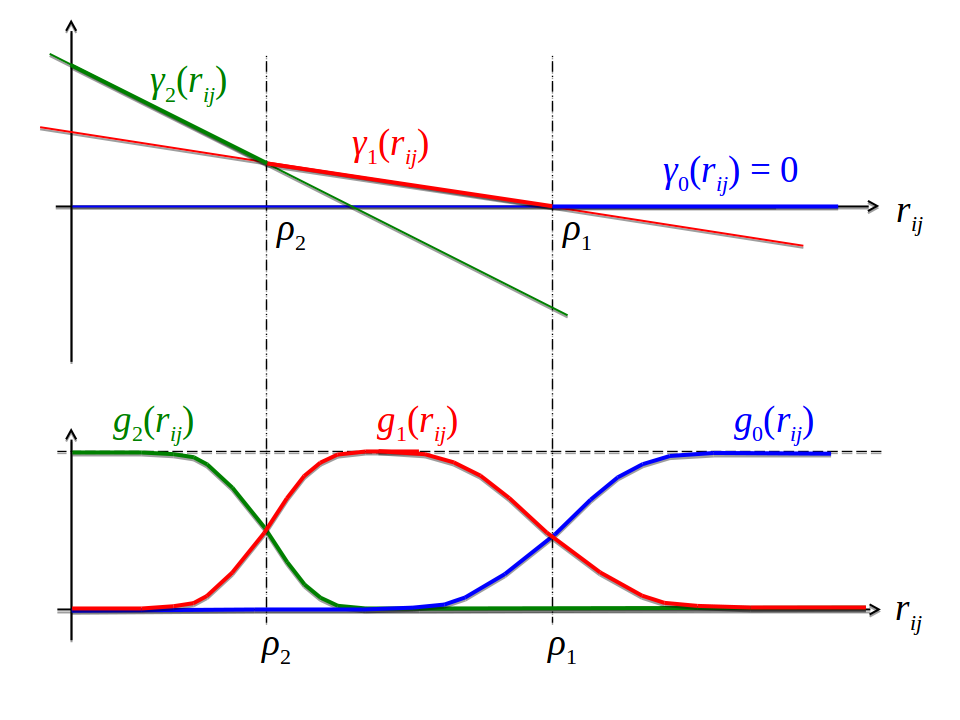
\includegraphics[width=0.5\linewidth]{img/theory/softmax_linear_fct} \caption{The Gaussian mixture coefficients
\(g_k(\rij)\) of \(p(\wij|\rij)\) are modelled as softmax over linear
functions \(\gamma_k(\rij)\). \(\rho_k\) sets the transition point
between neighbouring components \(g_{k-1}(\rij)\) and \(g_k(\rij)\),
while \(\alpha_k\) quantifies the abruptness of the transition between
\(g_{k-1}(\rij)\) and \(g_k(\rij)\).}\label{fig:softmax-linear-fct}
\end{figure}

The functions \(g_k(\rij)\) remain invariant when adding an offset to
all \(\gamma_k(\rij)\). This degeneracy can be removed by setting
\(\gamma_0(\rij) = 0\) (i.e., \(\alpha_0 = 0\) and \(\rho_0=0\)).
Further, the components are ordered, \(\rho_1> \ldots > \rho_K\) and it
is demanded that \(\alpha_k > 0\) for all \(k\). This ensures that for
\(\rij \rightarrow \infty\) we will obtain \(g_0(\rij) \rightarrow 1\)
and hence \(p(\w | \X) \rightarrow \Gauss(0, \sigma_0^2 \I )\).

The parameters \(\rho_k\) mark the transition points between the two
Gaussian mixture components \(k-1\) and \(k\), i.e., the points at which
the two components obtain equal weights. This follows from
\(\gamma_k(\rij) - \gamma_{k-1}(r) = \alpha_{t} ( \rij - \rho_{t})\) and
hence \(\gamma_{k-1}(\rho_k) = \gamma_k(\rho_k)\). A change in
\(\rho_k\) or \(\alpha_k\) only changes the behaviour of
\(g_{k-1}(\rij)\) and \(g_k(\rij)\) in the transition region around
\(\rho_k\). Therefore, this particular definition of \(\gamma_k(\rij)\)
makes the parameters \(\alpha_k\) and \(\rho_k\) as independent of each
other as possible, rendering the optimisation of these parameters more
efficient.

\subsection{\texorpdfstring{Training the Hyperparameters \(\rho_k\) and
\(\alpha_k\) for distance-dependent
prior}{Training the Hyperparameters \textbackslash{}rho\_k and \textbackslash{}alpha\_k for distance-dependent prior}}\label{training-the-hyperparameters-rho_k-and-alpha_k-for-distance-dependent-prior}

\section{Training Random Forest Contat
Prior}\label{training-random-forest-contat-prior}

\subsection{Sequence Derived Features}\label{seq-features}

Given a multiple sequence alignment of a protein family, various
sequence features can be derived that have been found to be informative
of a residue-residue contact.

In total there are \textbf{250} features that can be divided into
global, single position and pairwise features and are described in the
following sections. If not stated otherwise, \emph{weighted} features
have been computed using amino acid counts or amino acid frequencies
based on weighted sequences as described in section
\ref{seq-reweighting}.

\subsubsection{Global Features}\label{seq-features-global}

These features describe alignment characteristics. Every pair of
residues \((i,j)\) from the same protein will be attributed the same
feature.

\begin{longtable}[]{@{}rlc@{}}
\caption{Features characterizing the total alignment}\tabularnewline
\toprule
\begin{minipage}[b]{0.23\columnwidth}\raggedleft\strut
Feature\strut
\end{minipage} & \begin{minipage}[b]{0.50\columnwidth}\raggedright\strut
Description\strut
\end{minipage} & \begin{minipage}[b]{0.18\columnwidth}\centering\strut
No. Features per residue pair \((i, j)\)\strut
\end{minipage}\tabularnewline
\midrule
\endfirsthead
\toprule
\begin{minipage}[b]{0.23\columnwidth}\raggedleft\strut
Feature\strut
\end{minipage} & \begin{minipage}[b]{0.50\columnwidth}\raggedright\strut
Description\strut
\end{minipage} & \begin{minipage}[b]{0.18\columnwidth}\centering\strut
No. Features per residue pair \((i, j)\)\strut
\end{minipage}\tabularnewline
\midrule
\endhead
\begin{minipage}[t]{0.23\columnwidth}\raggedleft\strut
L\strut
\end{minipage} & \begin{minipage}[t]{0.50\columnwidth}\raggedright\strut
log of protein length L\strut
\end{minipage} & \begin{minipage}[t]{0.18\columnwidth}\centering\strut
1\strut
\end{minipage}\tabularnewline
\begin{minipage}[t]{0.23\columnwidth}\raggedleft\strut
N\strut
\end{minipage} & \begin{minipage}[t]{0.50\columnwidth}\raggedright\strut
number of sequences N\strut
\end{minipage} & \begin{minipage}[t]{0.18\columnwidth}\centering\strut
1\strut
\end{minipage}\tabularnewline
\begin{minipage}[t]{0.23\columnwidth}\raggedleft\strut
Neff\strut
\end{minipage} & \begin{minipage}[t]{0.50\columnwidth}\raggedright\strut
number of effective sequences Neff computed as the sum over sequence
weights (see section \ref{seq-reweighting})\strut
\end{minipage} & \begin{minipage}[t]{0.18\columnwidth}\centering\strut
1\strut
\end{minipage}\tabularnewline
\begin{minipage}[t]{0.23\columnwidth}\raggedleft\strut
gaps\strut
\end{minipage} & \begin{minipage}[t]{0.50\columnwidth}\raggedright\strut
average percentage of gaps over all positions\strut
\end{minipage} & \begin{minipage}[t]{0.18\columnwidth}\centering\strut
1\strut
\end{minipage}\tabularnewline
\begin{minipage}[t]{0.23\columnwidth}\raggedleft\strut
diversity\strut
\end{minipage} & \begin{minipage}[t]{0.50\columnwidth}\raggedright\strut
\(\frac{\sqrt{N}}{L}\), N=number of sequences, L=protein length\strut
\end{minipage} & \begin{minipage}[t]{0.18\columnwidth}\centering\strut
1\strut
\end{minipage}\tabularnewline
\begin{minipage}[t]{0.23\columnwidth}\raggedleft\strut
amino acid composition\strut
\end{minipage} & \begin{minipage}[t]{0.50\columnwidth}\raggedright\strut
weighted amino acid frequencies in alignment\strut
\end{minipage} & \begin{minipage}[t]{0.18\columnwidth}\centering\strut
20\strut
\end{minipage}\tabularnewline
\begin{minipage}[t]{0.23\columnwidth}\raggedleft\strut
secondary structure prediction\strut
\end{minipage} & \begin{minipage}[t]{0.50\columnwidth}\raggedright\strut
average three state propensities PSIPRED
(v4.0){[}{\textbf{???}}{]}\strut
\end{minipage} & \begin{minipage}[t]{0.18\columnwidth}\centering\strut
3\strut
\end{minipage}\tabularnewline
\begin{minipage}[t]{0.23\columnwidth}\raggedleft\strut
secondary structure prediction\strut
\end{minipage} & \begin{minipage}[t]{0.50\columnwidth}\raggedright\strut
average three state propensities Netsurfp
(v1.0){[}{\textbf{???}}{]}\strut
\end{minipage} & \begin{minipage}[t]{0.18\columnwidth}\centering\strut
3\strut
\end{minipage}\tabularnewline
\begin{minipage}[t]{0.23\columnwidth}\raggedleft\strut
contact prior protein length\strut
\end{minipage} & \begin{minipage}[t]{0.50\columnwidth}\raggedright\strut
simple contact predictor based on expected number of contacts per
protein with respect to protein length (see next subsection
\ref{contact-prior-protein-length})\strut
\end{minipage} & \begin{minipage}[t]{0.18\columnwidth}\centering\strut
1\strut
\end{minipage}\tabularnewline
\bottomrule
\end{longtable}

There are in total \textbf{32} global alignment features.

\subsubsection{Single Position Features}\label{seq-features-single}

These features describe characteristics of a single alignment column.
Every residue pair \((i,j)\) will be described by two features, once for
each position.

\begin{longtable}[]{@{}rlc@{}}
\caption{Single Position Sequence Features}\tabularnewline
\toprule
\begin{minipage}[b]{0.23\columnwidth}\raggedleft\strut
Feature\strut
\end{minipage} & \begin{minipage}[b]{0.50\columnwidth}\raggedright\strut
Description\strut
\end{minipage} & \begin{minipage}[b]{0.18\columnwidth}\centering\strut
No. Features per residue pair \((i, j)\)\strut
\end{minipage}\tabularnewline
\midrule
\endfirsthead
\toprule
\begin{minipage}[b]{0.23\columnwidth}\raggedleft\strut
Feature\strut
\end{minipage} & \begin{minipage}[b]{0.50\columnwidth}\raggedright\strut
Description\strut
\end{minipage} & \begin{minipage}[b]{0.18\columnwidth}\centering\strut
No. Features per residue pair \((i, j)\)\strut
\end{minipage}\tabularnewline
\midrule
\endhead
\begin{minipage}[t]{0.23\columnwidth}\raggedleft\strut
shannon entropy (20 states)\strut
\end{minipage} & \begin{minipage}[t]{0.50\columnwidth}\raggedright\strut
\(- \sum_{a=1}^{20} p_a \log p_a\)\strut
\end{minipage} & \begin{minipage}[t]{0.18\columnwidth}\centering\strut
2\strut
\end{minipage}\tabularnewline
\begin{minipage}[t]{0.23\columnwidth}\raggedleft\strut
shannon entropy (21 states)\strut
\end{minipage} & \begin{minipage}[t]{0.50\columnwidth}\raggedright\strut
\(- \sum_{a=1}^{21} p_a \log p_a\)\strut
\end{minipage} & \begin{minipage}[t]{0.18\columnwidth}\centering\strut
2\strut
\end{minipage}\tabularnewline
\begin{minipage}[t]{0.23\columnwidth}\raggedleft\strut
kullback leibler divergence\strut
\end{minipage} & \begin{minipage}[t]{0.50\columnwidth}\raggedright\strut
between weighted observed and background amino acid frequencies
{[}{\textbf{???}}{]}\strut
\end{minipage} & \begin{minipage}[t]{0.18\columnwidth}\centering\strut
2\strut
\end{minipage}\tabularnewline
\begin{minipage}[t]{0.23\columnwidth}\raggedleft\strut
jennson shannon divergence\strut
\end{minipage} & \begin{minipage}[t]{0.50\columnwidth}\raggedright\strut
between weighted observed and background amino acid frequencies
{[}{\textbf{???}}{]}\strut
\end{minipage} & \begin{minipage}[t]{0.18\columnwidth}\centering\strut
2\strut
\end{minipage}\tabularnewline
\begin{minipage}[t]{0.23\columnwidth}\raggedleft\strut
PSSM\strut
\end{minipage} & \begin{minipage}[t]{0.50\columnwidth}\raggedright\strut
log odds ratio of weighted observed and background amino acid
frequencies {[}{\textbf{???}}{]}\strut
\end{minipage} & \begin{minipage}[t]{0.18\columnwidth}\centering\strut
40\strut
\end{minipage}\tabularnewline
\begin{minipage}[t]{0.23\columnwidth}\raggedleft\strut
secondary structure prediction\strut
\end{minipage} & \begin{minipage}[t]{0.50\columnwidth}\raggedright\strut
three state propensities PSIPRED (v4.0) {[}{\textbf{???}}{]}\strut
\end{minipage} & \begin{minipage}[t]{0.18\columnwidth}\centering\strut
6\strut
\end{minipage}\tabularnewline
\begin{minipage}[t]{0.23\columnwidth}\raggedleft\strut
secondary structure prediction\strut
\end{minipage} & \begin{minipage}[t]{0.50\columnwidth}\raggedright\strut
three state propensities Netsurfp (v1.0) {[}{\textbf{???}}{]}\strut
\end{minipage} & \begin{minipage}[t]{0.18\columnwidth}\centering\strut
6\strut
\end{minipage}\tabularnewline
\begin{minipage}[t]{0.23\columnwidth}\raggedleft\strut
solvent accessibility prediction\strut
\end{minipage} & \begin{minipage}[t]{0.50\columnwidth}\raggedright\strut
RSA and RSA Z-score Netsurfp (v1.0) {[}{\textbf{???}}{]}\strut
\end{minipage} & \begin{minipage}[t]{0.18\columnwidth}\centering\strut
4\strut
\end{minipage}\tabularnewline
\begin{minipage}[t]{0.23\columnwidth}\raggedleft\strut
relative position in sequence\strut
\end{minipage} & \begin{minipage}[t]{0.50\columnwidth}\raggedright\strut
\(\frac{i}{L}\) for a protien of length \(L\)\strut
\end{minipage} & \begin{minipage}[t]{0.18\columnwidth}\centering\strut
2\strut
\end{minipage}\tabularnewline
\begin{minipage}[t]{0.23\columnwidth}\raggedleft\strut
number of ungapped sequences\strut
\end{minipage} & \begin{minipage}[t]{0.50\columnwidth}\raggedright\strut
\(\sum_n w_n I(x_{ni} \neq 20)\) for sequences \(x_n\) and sequence
weights \(w_n\)\strut
\end{minipage} & \begin{minipage}[t]{0.18\columnwidth}\centering\strut
2\strut
\end{minipage}\tabularnewline
\begin{minipage}[t]{0.23\columnwidth}\raggedleft\strut
percentage of gaps\strut
\end{minipage} & \begin{minipage}[t]{0.50\columnwidth}\raggedright\strut
\(\frac{\sum_n w_n I(x_{ni} = 20)}{N_{\text{eff}}}\) for sequences
\(x_n\) and sequence weights \(w_n\)\strut
\end{minipage} & \begin{minipage}[t]{0.18\columnwidth}\centering\strut
2\strut
\end{minipage}\tabularnewline
\begin{minipage}[t]{0.23\columnwidth}\raggedleft\strut
Average physico-chemical properties\strut
\end{minipage} & \begin{minipage}[t]{0.50\columnwidth}\raggedright\strut
Atchley Factors 1-5 {[}\protect\hyperlink{ref-Atchley2005}{94}{]}\strut
\end{minipage} & \begin{minipage}[t]{0.18\columnwidth}\centering\strut
10\strut
\end{minipage}\tabularnewline
\begin{minipage}[t]{0.23\columnwidth}\raggedleft\strut
Average physico-chemical properties\strut
\end{minipage} & \begin{minipage}[t]{0.50\columnwidth}\raggedright\strut
Polarity accordign to Grantham, 1974. Data taken from
\href{http://www.genome.jp/dbget-bin/www_bget?aaindex:GRAR740102}{AAindex
Database} {[}{\textbf{???}}{]}.\strut
\end{minipage} & \begin{minipage}[t]{0.18\columnwidth}\centering\strut
2\strut
\end{minipage}\tabularnewline
\begin{minipage}[t]{0.23\columnwidth}\raggedleft\strut
Average physico-chemical properties\strut
\end{minipage} & \begin{minipage}[t]{0.50\columnwidth}\raggedright\strut
Polarity according to Zimmermann et al., 1986. Data taken from
\href{http://www.genome.jp/dbget-bin/www_bget?aaindex:ZIMJ680103}{AAindex
Database} {[}{\textbf{???}}{]}.\strut
\end{minipage} & \begin{minipage}[t]{0.18\columnwidth}\centering\strut
2\strut
\end{minipage}\tabularnewline
\begin{minipage}[t]{0.23\columnwidth}\raggedleft\strut
Average physico-chemical properties\strut
\end{minipage} & \begin{minipage}[t]{0.50\columnwidth}\raggedright\strut
Isoelectric point according to Zimmermann et al., 1968. Data taken from
\href{http://www.genome.jp/dbget-bin/www_bget?aaindex:ZIMJ680104}{AAindex
Database} {[}{\textbf{???}}{]}.\strut
\end{minipage} & \begin{minipage}[t]{0.18\columnwidth}\centering\strut
2\strut
\end{minipage}\tabularnewline
\begin{minipage}[t]{0.23\columnwidth}\raggedleft\strut
Average physico-chemical properties\strut
\end{minipage} & \begin{minipage}[t]{0.50\columnwidth}\raggedright\strut
Hydrophobicity scale according to Wimley \& White, 1996. Data taken from
\href{https://www.cgl.ucsf.edu/chimera/docs/ContributedSoftware/defineattrib/wwHydrophobicity.txt}{UCSF
Chimera} {[}{\textbf{???}}{]}.\strut
\end{minipage} & \begin{minipage}[t]{0.18\columnwidth}\centering\strut
2\strut
\end{minipage}\tabularnewline
\begin{minipage}[t]{0.23\columnwidth}\raggedleft\strut
Average physico-chemical properties\strut
\end{minipage} & \begin{minipage}[t]{0.50\columnwidth}\raggedright\strut
Hydrophobicity index according to Kyte \& Doolittle, 1982. Data taken
from
\href{http://www.genome.jp/dbget-bin/www_bget?aaindex:KYTJ820101}{AAindex
Database} {[}{\textbf{???}}{]}.\strut
\end{minipage} & \begin{minipage}[t]{0.18\columnwidth}\centering\strut
2\strut
\end{minipage}\tabularnewline
\begin{minipage}[t]{0.23\columnwidth}\raggedleft\strut
Average physico-chemical properties\strut
\end{minipage} & \begin{minipage}[t]{0.50\columnwidth}\raggedright\strut
Hydrophobicity according to Cornette {[}{\textbf{???}}{]}.\strut
\end{minipage} & \begin{minipage}[t]{0.18\columnwidth}\centering\strut
2\strut
\end{minipage}\tabularnewline
\begin{minipage}[t]{0.23\columnwidth}\raggedleft\strut
Average physico-chemical properties\strut
\end{minipage} & \begin{minipage}[t]{0.50\columnwidth}\raggedright\strut
Bulkiness according to Zimmerman et al., 1968. Data taken from
\href{http://www.genome.jp/dbget-bin/www_bget?aaindex:ZIMJ680102}{AAindex
Database} {[}{\textbf{???}}{]}.\strut
\end{minipage} & \begin{minipage}[t]{0.18\columnwidth}\centering\strut
2\strut
\end{minipage}\tabularnewline
\begin{minipage}[t]{0.23\columnwidth}\raggedleft\strut
Average physico-chemical properties\strut
\end{minipage} & \begin{minipage}[t]{0.50\columnwidth}\raggedright\strut
Average volumes of residues according to Pontius et al., 1996. Data
taken from
\href{http://www.genome.jp/dbget-bin/www_bget?aaindex:PONJ960101}{AAindex
Database} {[}{\textbf{???}}{]}.\strut
\end{minipage} & \begin{minipage}[t]{0.18\columnwidth}\centering\strut
2\strut
\end{minipage}\tabularnewline
\bottomrule
\end{longtable}

There are in total \textbf{96} single sequence features.

Additionally, all single features will be computed within a window of
size 5. The window feature for center residue \(i\) will be computed as
the mean feature over residues \([i-2, \ldots, i, \ldots, i+2]\).
Whenever the window extends the range of the sequence (for \(i\!<\!2\)
and \(i\!>\!(L-2)\)), the window feature will be computed only for valid
sequence positions. This results in additional \textbf{96} window
features.

\subsubsection{Pairwise Features}\label{seq-features-pairwise}

These features are computed for every pair of columns \((i, j)\) in the
alignment with \(i<j\).

\begin{longtable}[]{@{}rlc@{}}
\caption{Pairwise Sequence Features}\tabularnewline
\toprule
\begin{minipage}[b]{0.23\columnwidth}\raggedleft\strut
Feature\strut
\end{minipage} & \begin{minipage}[b]{0.50\columnwidth}\raggedright\strut
Description\strut
\end{minipage} & \begin{minipage}[b]{0.18\columnwidth}\centering\strut
No. Features per residue pair \((i, j)\)\strut
\end{minipage}\tabularnewline
\midrule
\endfirsthead
\toprule
\begin{minipage}[b]{0.23\columnwidth}\raggedleft\strut
Feature\strut
\end{minipage} & \begin{minipage}[b]{0.50\columnwidth}\raggedright\strut
Description\strut
\end{minipage} & \begin{minipage}[b]{0.18\columnwidth}\centering\strut
No. Features per residue pair \((i, j)\)\strut
\end{minipage}\tabularnewline
\midrule
\endhead
\begin{minipage}[t]{0.23\columnwidth}\raggedleft\strut
sequence separation\strut
\end{minipage} & \begin{minipage}[t]{0.50\columnwidth}\raggedright\strut
\(j-i\)\strut
\end{minipage} & \begin{minipage}[t]{0.18\columnwidth}\centering\strut
1\strut
\end{minipage}\tabularnewline
\begin{minipage}[t]{0.23\columnwidth}\raggedleft\strut
gaps\strut
\end{minipage} & \begin{minipage}[t]{0.50\columnwidth}\raggedright\strut
pairwise percentage of gaps using weighted sequences\strut
\end{minipage} & \begin{minipage}[t]{0.18\columnwidth}\centering\strut
1\strut
\end{minipage}\tabularnewline
\begin{minipage}[t]{0.23\columnwidth}\raggedleft\strut
number of ungapped sequences\strut
\end{minipage} & \begin{minipage}[t]{0.50\columnwidth}\raggedright\strut
\(\sum_n w_n I(x_{ni} \! \neq \! 20, x_{nj} \! \neq \! 20)\) for
sequences \(x_n\) and sequence weights \(w_n\)\strut
\end{minipage} & \begin{minipage}[t]{0.18\columnwidth}\centering\strut
1\strut
\end{minipage}\tabularnewline
\begin{minipage}[t]{0.23\columnwidth}\raggedleft\strut
correlation physico-chemical features\strut
\end{minipage} & \begin{minipage}[t]{0.50\columnwidth}\raggedright\strut
pairwise correlation of all physico-chemical properties listed in
\ref{seq-features-single}\strut
\end{minipage} & \begin{minipage}[t]{0.18\columnwidth}\centering\strut
13\strut
\end{minipage}\tabularnewline
\begin{minipage}[t]{0.23\columnwidth}\raggedleft\strut
pairwise potential\strut
\end{minipage} & \begin{minipage}[t]{0.50\columnwidth}\raggedright\strut
Average quasi-chemical energy of interactions in an average buried
environment. Data taken from
\href{http://www.genome.jp/dbget-bin/www_bget?aaindex:MIYS990107}{AAindex
Database} {[}{\textbf{???}}{]}.\strut
\end{minipage} & \begin{minipage}[t]{0.18\columnwidth}\centering\strut
1\strut
\end{minipage}\tabularnewline
\begin{minipage}[t]{0.23\columnwidth}\raggedleft\strut
pairwise potential\strut
\end{minipage} & \begin{minipage}[t]{0.50\columnwidth}\raggedright\strut
Average quasi-chemical energy of transfer of amino acids from water to
the protein environment. Data taken from
\href{http://www.genome.jp/dbget-bin/www_bget?aaindex:MIYS990106}{AAindex
Database} {[}{\textbf{???}}{]}.\strut
\end{minipage} & \begin{minipage}[t]{0.18\columnwidth}\centering\strut
1\strut
\end{minipage}\tabularnewline
\begin{minipage}[t]{0.23\columnwidth}\raggedleft\strut
pairwise potential\strut
\end{minipage} & \begin{minipage}[t]{0.50\columnwidth}\raggedright\strut
Average general contact potential by Li\&Fang
{[}\protect\hyperlink{ref-Li2011}{95}{]}\strut
\end{minipage} & \begin{minipage}[t]{0.18\columnwidth}\centering\strut
1\strut
\end{minipage}\tabularnewline
\begin{minipage}[t]{0.23\columnwidth}\raggedleft\strut
pairwise potential\strut
\end{minipage} & \begin{minipage}[t]{0.50\columnwidth}\raggedright\strut
Average statistical potential from residue pairs in beta-sheets by
Zhu\&Braun {[}\protect\hyperlink{ref-Zhu1999}{96}{]}\strut
\end{minipage} & \begin{minipage}[t]{0.18\columnwidth}\centering\strut
1\strut
\end{minipage}\tabularnewline
\begin{minipage}[t]{0.23\columnwidth}\raggedleft\strut
joint\_shannon\_entropy (20 state)\strut
\end{minipage} & \begin{minipage}[t]{0.50\columnwidth}\raggedright\strut
\(- \sum_{a=1}^{20}\sum_{b=1}^{20} p(a,b) \log p(a,b)\)\strut
\end{minipage} & \begin{minipage}[t]{0.18\columnwidth}\centering\strut
1\strut
\end{minipage}\tabularnewline
\begin{minipage}[t]{0.23\columnwidth}\raggedleft\strut
joint\_shannon\_entropy (21 state)\strut
\end{minipage} & \begin{minipage}[t]{0.50\columnwidth}\raggedright\strut
\(- \sum_{a=1}^{21}\sum_{b=1}^{21} p(a,b) \log p(a,b)\)\strut
\end{minipage} & \begin{minipage}[t]{0.18\columnwidth}\centering\strut
1\strut
\end{minipage}\tabularnewline
\begin{minipage}[t]{0.23\columnwidth}\raggedleft\strut
mutual information (MI)\strut
\end{minipage} & \begin{minipage}[t]{0.50\columnwidth}\raggedright\strut
several variants: MI with pseudo-counts, MI with pseudo-counts + APC,
normalized MI\strut
\end{minipage} & \begin{minipage}[t]{0.18\columnwidth}\centering\strut
3\strut
\end{minipage}\tabularnewline
\begin{minipage}[t]{0.23\columnwidth}\raggedleft\strut
OMES\strut
\end{minipage} & \begin{minipage}[t]{0.50\columnwidth}\raggedright\strut
according to Fodor\&Aldrich {[}\protect\hyperlink{ref-Fodor2004a}{97}{]}
with and without APC\strut
\end{minipage} & \begin{minipage}[t]{0.18\columnwidth}\centering\strut
2\strut
\end{minipage}\tabularnewline
\bottomrule
\end{longtable}

There are in total \textbf{26} pairwise sequence features.

\subsubsection{Protein length dependent Contact
Prior}\label{contact-prior-protein-length}

The average number of contats per residue, computed as the observed
number of contacts divided by protein length L, has a non-linear
relationship with protein length L as can be seen in Figure
\ref{fig:avg-nr-contacts-per-residue-vs-protein-length}.






\begin{figure}

{\centering 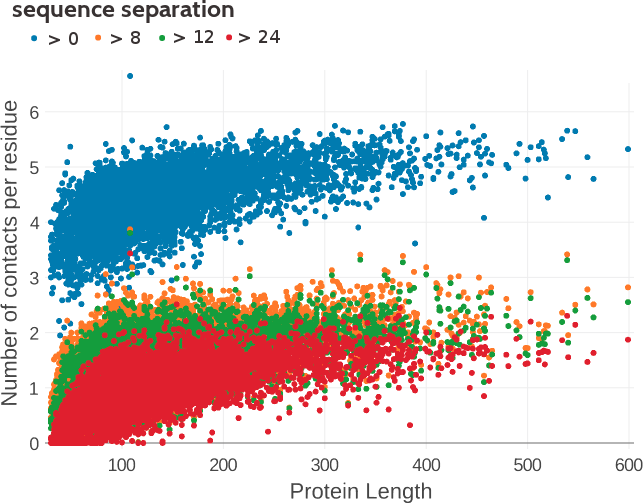
\includegraphics[width=0.8\linewidth]{img/random_forest_contact_prior/no_contacts_per_residue_vs_protein_length_thr8} 

}

\caption{Observed
number of contacts per residue has a non-linear relationship with
protein length. Distribution is shown for several thresholds of sequence
separation.}\label{fig:avg-nr-contacts-per-residue-vs-protein-length}
\end{figure}

In log space, the average number of contats per residue can be fitted
with a linear regression (see Figure
\ref{fig:avg-nr-contacts-per-residue-vs-log-protein-length-linfit}) and
yields the following functions:

\begin{itemize}
\tightlist
\item
  \(f(L) = 1.556 + 0.596 \log (L)\) for sequence separation of 0
  positions
\item
  \(f(L) = -1.273 + 0.59 \log (L)\) for sequence separation of 8
  positions
\item
  \(f(L) = -1.567 + 0.615 \log (L)\) for sequence separation of 12
  positions
\item
  \(f(L) = -2.0 + 0.624 \log (L)\) for sequence separation of 24
  positions
\end{itemize}

A simple contact predictor can be formulated as the ratio of the
expected number of contacts per residue, given by \(f(L)\), and the
possible number of contacts per residue which is \(L-1\),

\[
p(r_{ij} = 1 | L) = \frac{f(L)}{L-1} \; ,
\]

with \(r_{ij}=1\) representing a contact between residue \(i\) and
\(j\).

(ref:caption-avg-nr-contacts-per-residue-vs-log-protein-length-linfit)
Linear regression fits for average number of contats per residue on
logarithm of protein length. Distribution and linear regression fits are
shown for different sequence separation thresholds.

\begin{figure}

{\centering 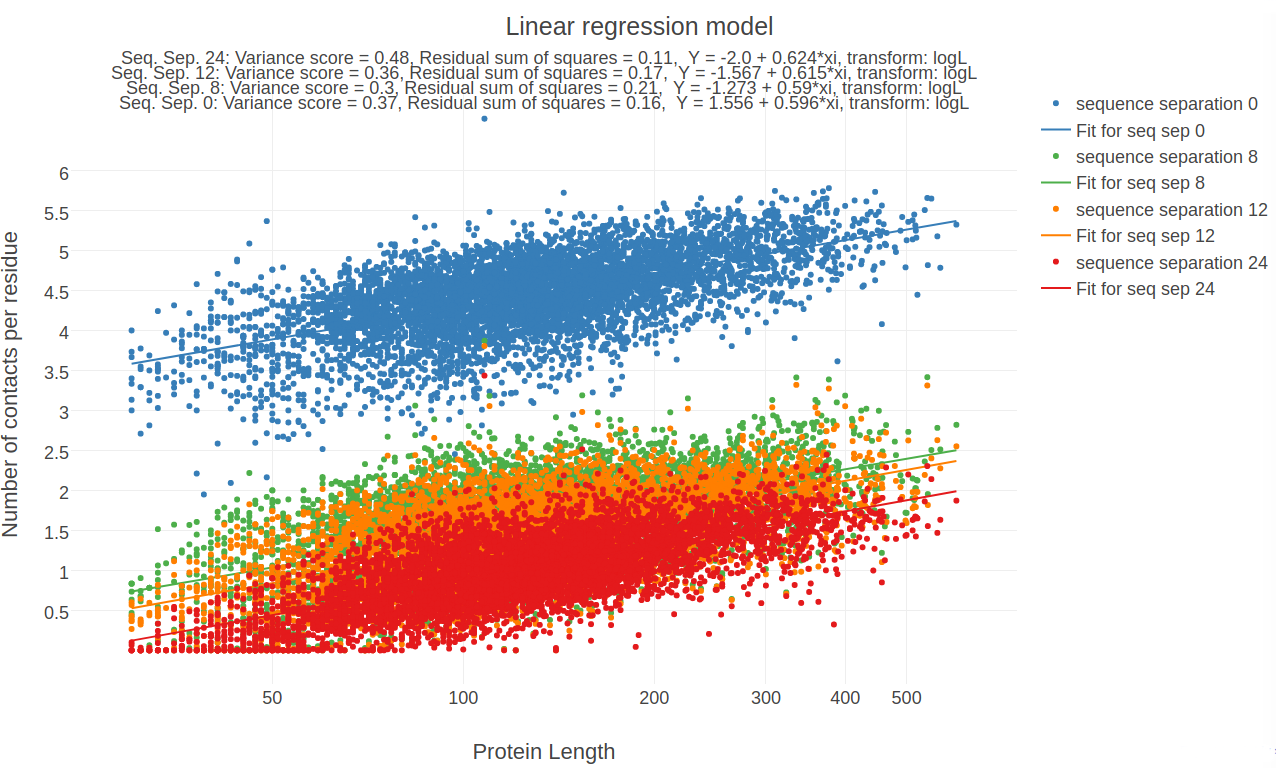
\includegraphics[width=0.9\linewidth]{img/random_forest_contact_prior/model_linreg_transformlogL_no_contacts_per_residue_vs_protein_length_thr8} 

}

\caption{(ref:caption-avg-nr-contacts-per-residue-vs-log-protein-length-linfit)}\label{fig:avg-nr-contacts-per-residue-vs-log-protein-length-linfit}
\end{figure}

\subsection{Hyperparameter Optimization for Random Forest
Prior}\label{rf-hyperparameter-optimization}

There are several parameters that need to be tuned in such a way as to
obtain a trade-off between model performance and size of the model.
Apart from requiring a lot of disk space, the larger the model becomes,
the longer it will take to train and to make predictions:

The module \texttt{ensemble.RandomForestClassifier} in the Python
package \texttt{sklearn\ (v.\ 0.19)} was used to learn random forest
classifiers over sequence features described in section
\ref{seq-features} {[}{\textbf{???}}{]}. Hyperparamters of the random
forest were optimized with a grid search over parameter space using
5-fold cross-validation on a dataset with 50.000 residue pairs
\(< 8 \AA\) (``contacts''``) and 250.000 residue pairs \(> 8 \AA\)
(''non-contacts``) using a window size of 5 for single position features
as described in section \ref{seq-features-single}.

First of all, I performed grid search over the parameters
\emph{n\_estimators}, defining the number of trees in the forest and
\emph{max\_features}, defining the number of randomly selected features
considerd for each split using the following settings:

\begin{itemize}
\tightlist
\item
  \emph{n\_estimators}: {[}100,500,1000{]}
\item
  \emph{max\_features}: {[}`sqrt', `log2', None{]}
\end{itemize}

Figure \ref{fig:rf-gridsearch-nestimators-maxfeatures} visualizes the
results of the grid search. Considering only \(\log_2 \approx 8\)
features for every split yields highest precision averaged over the five
cross-validation runs regardless of how many trees are learned. I chose
\emph{n\_estimators} = 1000 and \emph{max\_features} = log2 for further
analysis.







\begin{figure}

{\centering 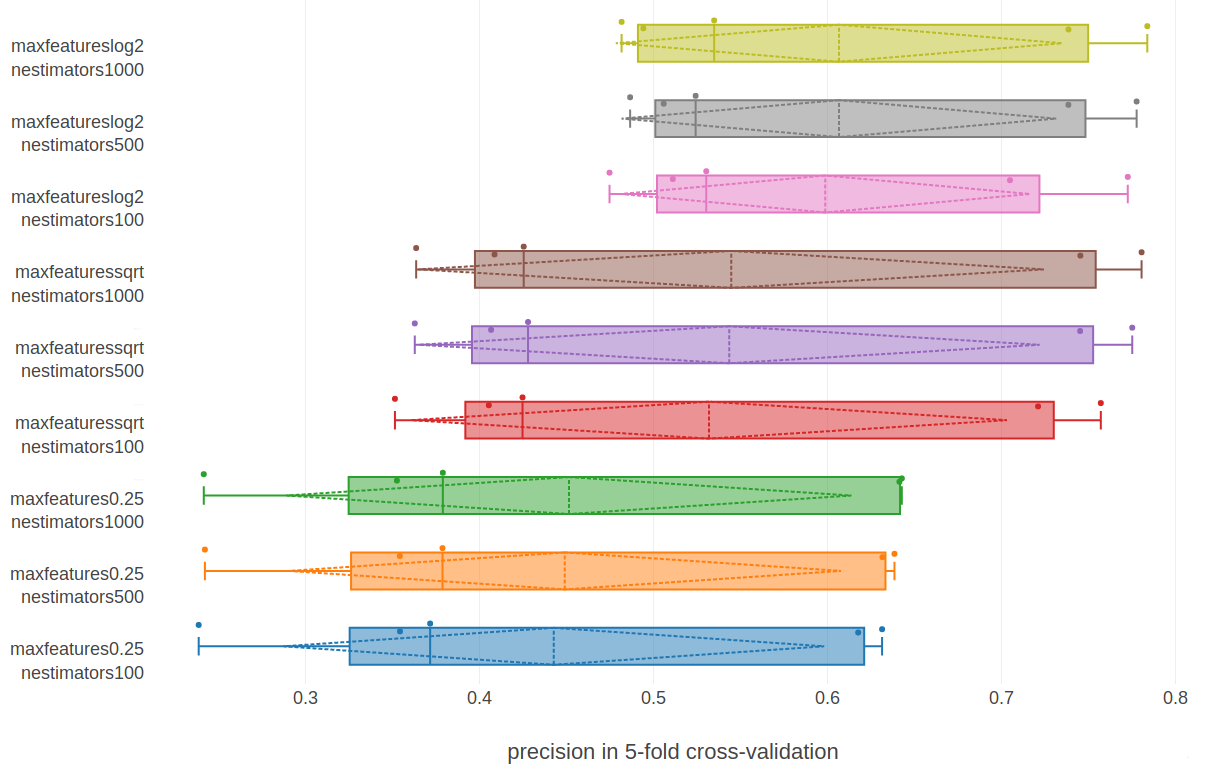
\includegraphics[width=0.9\linewidth]{img/random_forest_contact_prior/gridsearch/grid_search_cv_results_precision_random_forest_notitle_nrestimators_maxfeatures} 

}

\caption{Distribution of
precision for 5-fold cross-validation of a grid search over parameters
\emph{n\_estiamtors} and \emph{max\_features}. Using 1000 trees and
randomly selecting \(\log_2\) feautures at every split yields highest
mean precision over the five runs.}\label{fig:rf-gridsearch-nestimators-maxfeatures}
\end{figure}

Next, I optimized the parameters \emph{min\_samples\_leaf} defining the
minimum number of samples required to be at a leaf node and
\emph{max\_depth} defining the maximum depth of the trees using the
following settings:

\begin{itemize}
\tightlist
\item
  \emph{min\_samples\_leaf}: {[}1, 10, 100{]}
\item
  \emph{max\_depth}: {[}10, 100, 1000, None{]}
\end{itemize}

Evluated using precision for out-of-bag samples???? PLOT GRID SEARCH
RESULTS

Using the optimal setting of hyperparameters
(\texttt{n\_estimators=1000,\ min\_samples\_leaf=100,\ max\_depth=100,\ max\_features=sqrt})
obtained from the grid search, cross-validation was used to optimize the
window-size of features (see section\ref{seq-features-single}):

\begin{itemize}
\tightlist
\item
  window size: {[}5, 7, 9, 11{]}
\end{itemize}

PLOT PRECISISON FOR WINDOW SIZES

The problem of predicting contacting residues is a highly imbalanced
problem with approximately 5\% contacts.








\begin{figure}

{\centering 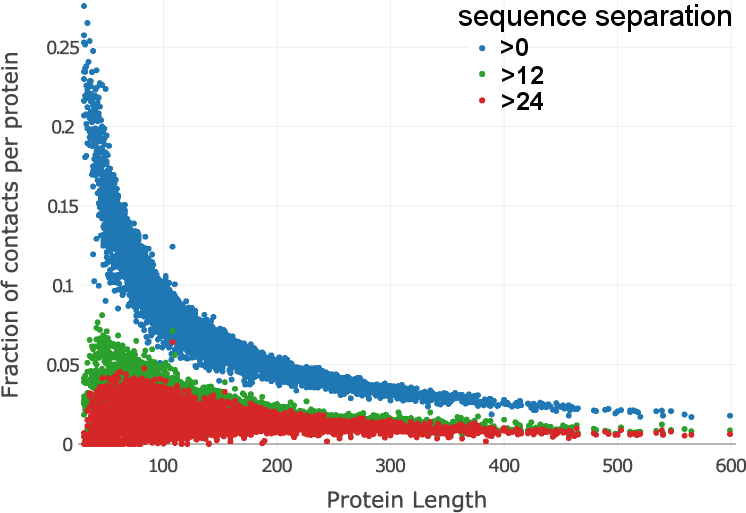
\includegraphics[width=0.8\linewidth]{img/random_forest_contact_prior/fraction_contacts_vs_protein_length_thr8} 

}

\caption{Fraction of contacts
among all possible contacts (\(\frac{L(L-1)}{2}\)) in a protein against
protein length L. The distribution has a non-linear relationship. At a
sequence separation threshold \textgreater{}8 positions the fraction of
contacts for intermediate size proteins with length \textgreater{}100 is
approximately 2\%.}\label{fig:fraction-contacts-vs-protein-length}
\end{figure}

Therefore, the ratio of contacts to non-contacts was optimized with
5-fold crossvalidation while performing a grid seardch over the
\texttt{class-weight} parameter which assigns a weight to each
datasample according to the class label.

\begin{itemize}
\tightlist
\item
  varying class ratios using equal amount of total data:
\item
  1:1 = 250 000 : 250 000
\item
  1:3 = 125 000 : 375 000
\item
  1:5 = 85 000 : 415 000
\item
  1:10 = 45 000 : 455 000
\item
  `class\_weight': {[} None, \# equal class weights ``balanced'', \#
  n\_samples / (n\_classes * np.bincount(y)) \{0: 0.6, 1: 3\}, \#
  ==\textgreater{} ``balanced'' for ratio 1:5 \{0: 0.55, 1: 5.5\}, \#
  ==\textgreater{} ``balanced'' for ratio 1:10 \{0: 0.525, 1: 10.5\}, \#
  ==\textgreater{} ``balanced'' for ratio 1:20 \{0: 10.5, 1: 0.525\} \#
  ==\textgreater{} ``balanced'' for ratio 20:1 (sanity check) {]}
\end{itemize}

PLOT GRID SEARCH RESULTS FOR EVERY DATASET (=4 plots)

\subsection{Feature Selection}\label{rf-feature-selection}

Many features obtain low \emph{Gini importance} scores and can most
likely be removed from the data set, thus also reducig model complexity.
It has been found, that prediction performance might even increase after
removing the most irrelevant feaures {[}{\textbf{???}}{]}. For example,
during the development of \emph{EPSILON-CP}, a deep neural network
method for contact prediction, the authors performed feature selection
using boosted trees. By removing 75\% of the most non-informative
features (mostly attributed to amino acid composition), the performance
of their predictor increased slightly {[}{\textbf{???}}{]}.

I therefore developed a feature selection pipeline with which to retrain
the random forest on subsets of features. As subsets I chose those
feautures with \emph{Gini importance} larger than the
\(\{10, 30, 50, 70, 90\}\)-percentile of \emph{Gini importance} values.
Performance is then evaluated for the models trained on these subsets of
features.

\subsection{Using Pseudo-likelihood Coevolution Score as Additional
Feature}\label{rf-with-pll-score}

In addition to the 250 sequence derived features, the pseudo-likelihood
contact score (L2norm + APC) is used as a feature. The random forest was
trained on 100.000 residue pairs in contact
(\(\Delta \Cb < 8 \AA \; \;\)) and 500.000 residue pairs not in contact
(\(\Delta \Cb > 8 \AA \; \;\)) using the cross-validated hyperparameters
as described in the last section.

The pseudo-likelihood contact score comprises by far the most important
feature as can be seen in the following Figure
\ref{fig:feature-importance-rf-with-pll-score}.






\begin{figure}

{\centering 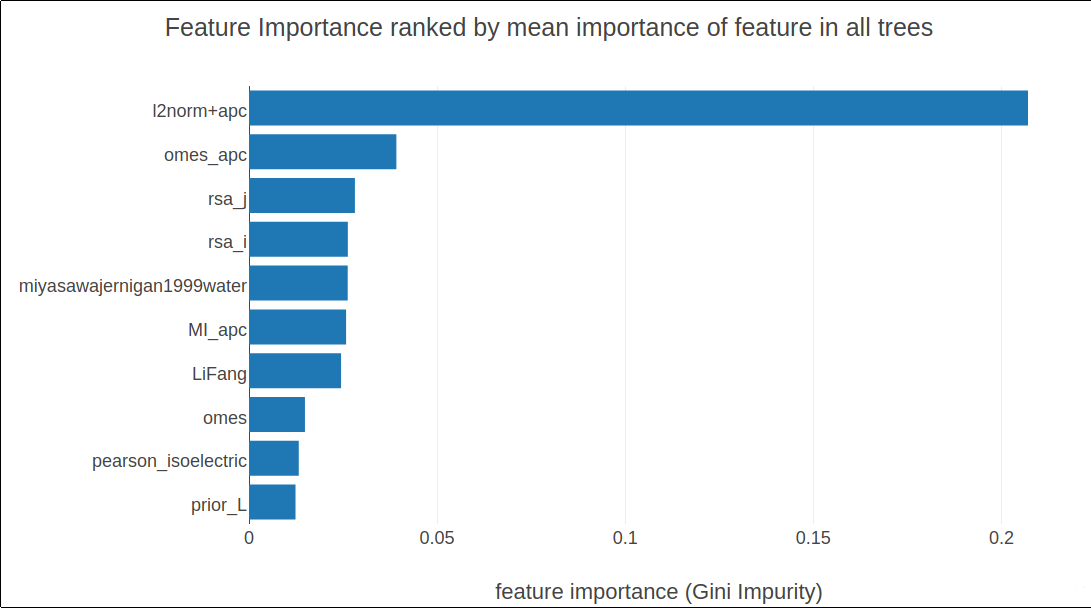
\includegraphics[width=0.9\linewidth]{img/random_forest_contact_prior/feature_plll2norm_random_forest_nestimators1000_maxfeaturesauto_251features_top} 

}

\caption{Most important
features in the random forest model. Features are ranked according to
Gini importance which is the mean decrease in Gini impurity over all
splits and all trees in the forest.}\label{fig:feature-importance-rf-with-pll-score}
\end{figure}

Training the model only on the 26 most important features improves
precision of the model compared to using the full feature set as is
illustrated in the following figure
\ref{fig:feature-importance-rf-with-pll-score}.








\begin{figure}

{\centering 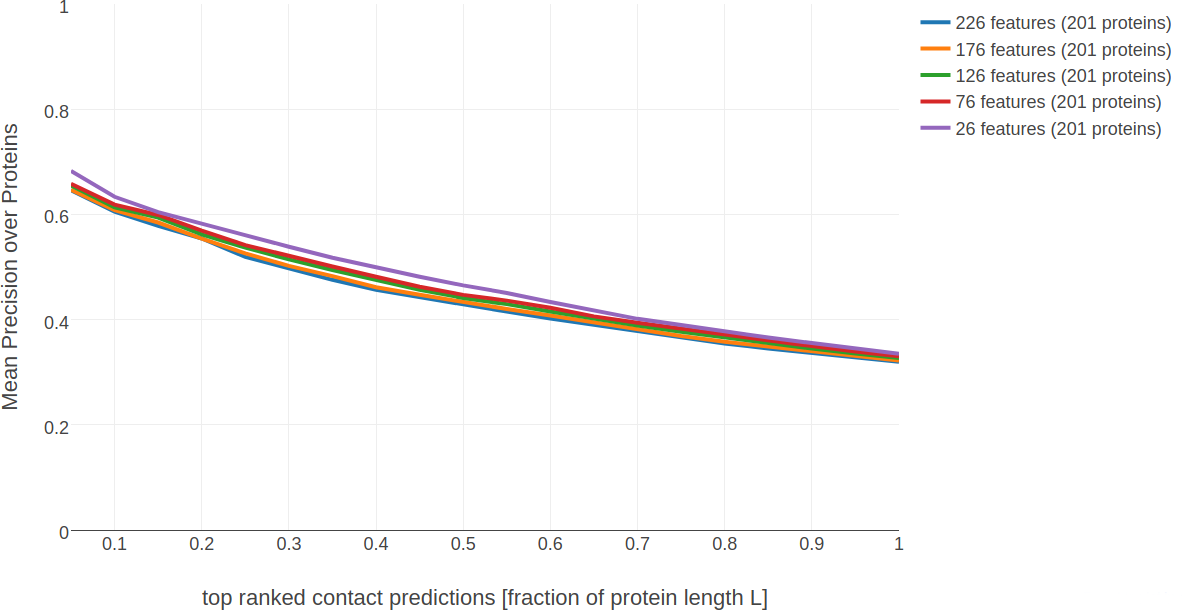
\includegraphics[width=0.9\linewidth]{img/random_forest_contact_prior/precision_vs_rank_featureselection_plll2norm_random_forest_nestimators1000_maxfeaturesauto_26features_notitle} 

}

\caption{Mean precision over
proteins in testset for the top ranked contacts for variaous random
forest models trained on subsets of features. Subsets of features have
been selected as described in section \ref{rf-feature-selection}.
Learning a random forest model on the 26 most important features yields
the best model with respect to precision.}\label{fig:feature-selection-rf-with-pll-score}
\end{figure}

\appendix


\hypertarget{abbrev}{\chapter{Abbreviations}\label{abbrev}}

\textbf{APC} Avarage Product Correction

\textbf{CASP} Critical Assessment of protein Structure Prediction

\textbf{CD} Contrastive Divergence

\textbf{DCA} Direct Coupling Analysis

\textbf{DI} Direct Information

\textbf{EM} electron microscopy

\textbf{IDP} intrinsically disordered proteins

\textbf{MAP} Maximum a posteriori

\textbf{MI} mutual information

\textbf{ML} Maximum-Likelihood

\textbf{MLE} Maximum-Likelihood Estimate

\textbf{MRF} Markov-Random Field

\textbf{MSA} Multiple Sequence Alignment

\textbf{Neff} Number of effective sequences

\textbf{PCD} Persistent Contrastive Divergence

\textbf{PDB} protein data bank

\%\%\%\% used as: \protect\hyperlink{abbrev}{MRF}

\chapter{Dataset Properties}\label{dataset-properties}

The following figures display various statistics about the dataset used
throughout this thesis. See section \ref{dataset} for information on how
this dataset has been generated.

\section{Alignment Diversity}\label{alignment-diversity}




\begin{figure}
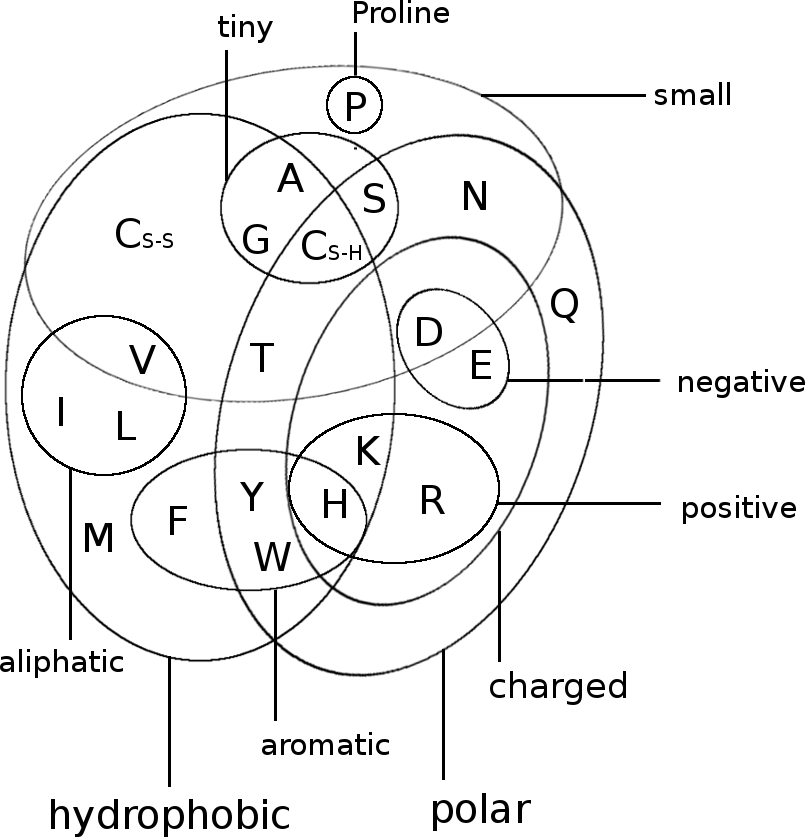
\includegraphics[width=1\linewidth]{img/amino_acid_physico_chemical_properties_venn_diagramm} \caption{Distribution of alignment diversity
(\(=\sqrt(\frac{N}{L})\)) in the dataset an its ten subsets.}\label{fig:dataset-diversity}
\end{figure}

\section{Proportion of Gaps in
Alignment}\label{proportion-of-gaps-in-alignment}




\begin{figure}
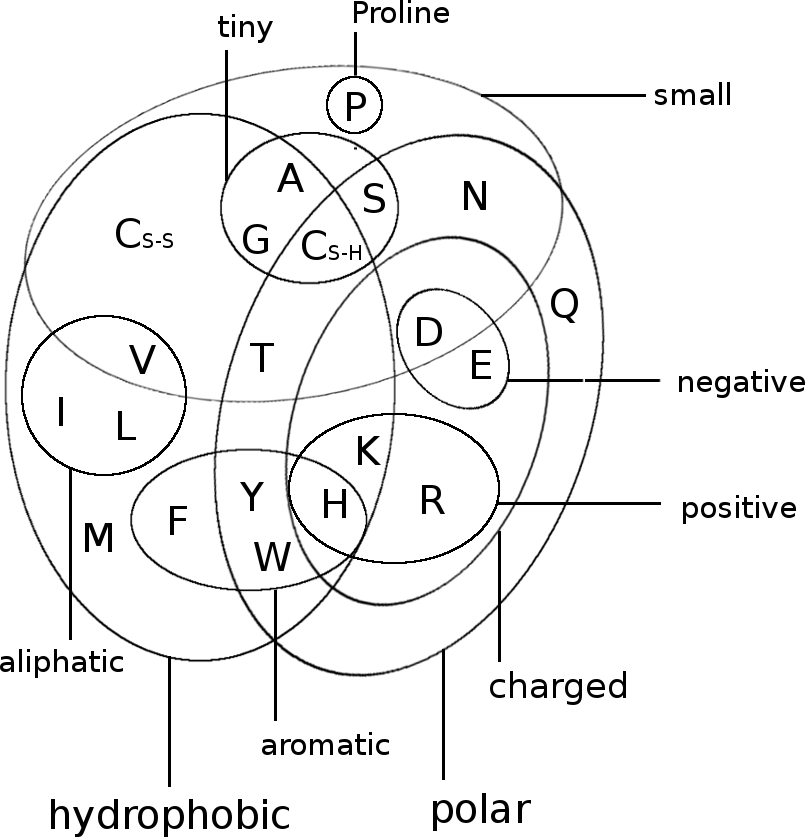
\includegraphics[width=1\linewidth]{img/amino_acid_physico_chemical_properties_venn_diagramm} \caption{Distribution of gap percentage of alignments in the
dataset an its ten subsets.}\label{fig:dataset-gaps}
\end{figure}

\section{Alignment Size (number of
sequences)}\label{alignment-size-number-of-sequences}




\begin{figure}
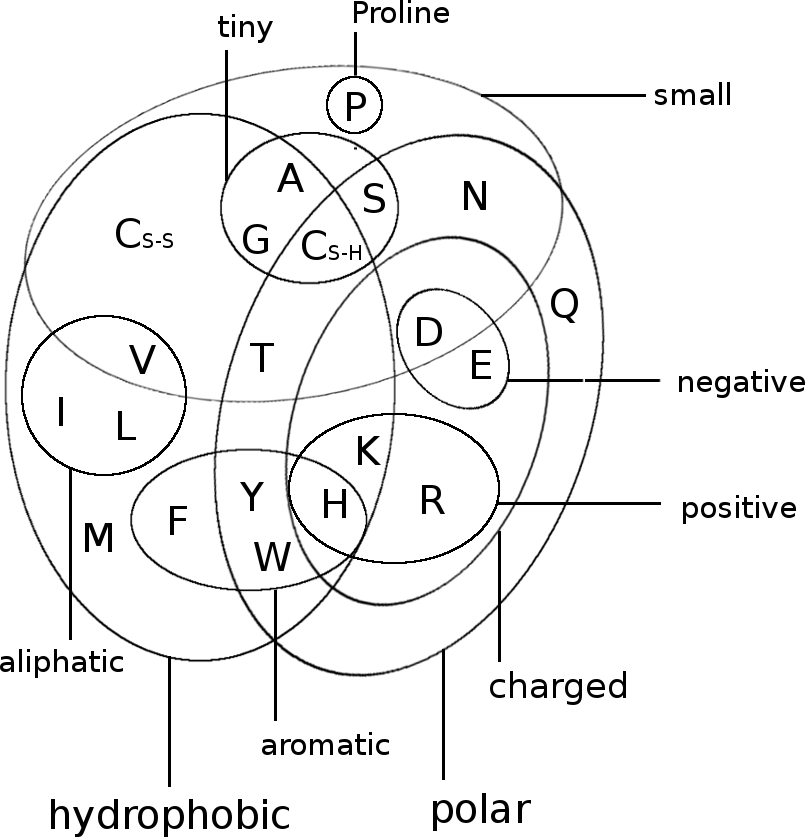
\includegraphics[width=1\linewidth]{img/amino_acid_physico_chemical_properties_venn_diagramm} \caption{Distribution of alignment size (number of
sequences N) in the dataset an its ten subsets.}\label{fig:dataset-alignment-size}
\end{figure}

\section{Protein Length}\label{protein-length}




\begin{figure}
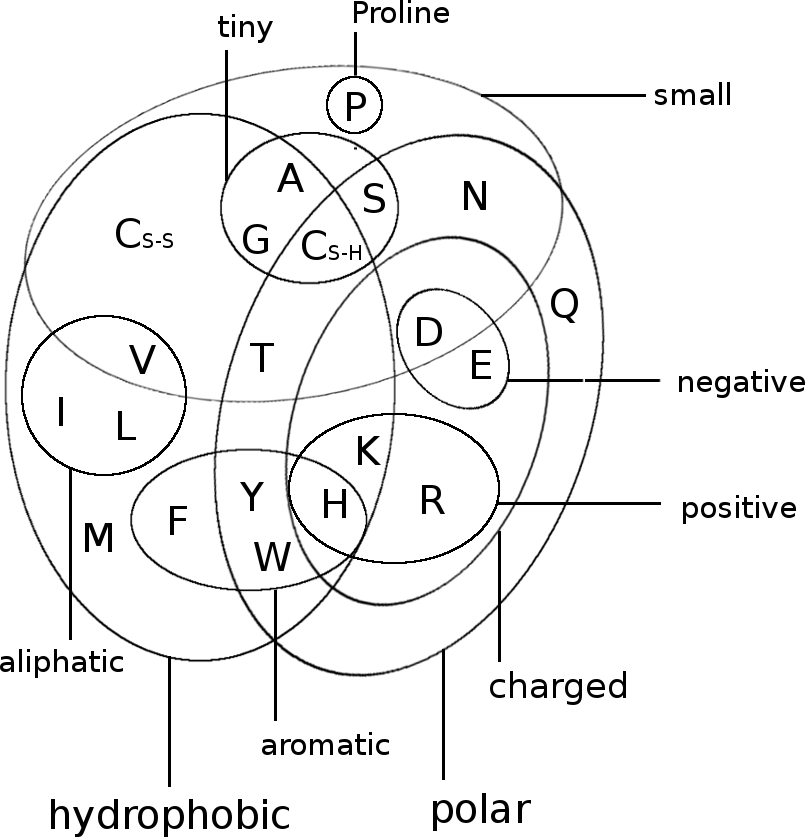
\includegraphics[width=1\linewidth]{img/amino_acid_physico_chemical_properties_venn_diagramm} \caption{Distribution of protein length L in the
dataset an its ten subsets.}\label{fig:dataset-protein-length}
\end{figure}

\chapter{Amino Acid Interaction Preferences Reflected in Coupling
Matrices}\label{amino-acid-interaction-preferences-reflected-in-coupling-matrices}

\section{Pi-Cation interactions}\label{pi-cation}

Figure \ref{fig:coupling-matrix-pication-pymol} shows a Tyrosine and a
Lysine residue forming a cation-\(\pi\) interaction in protein 2ayd. The
corresponding coupling matrix in figure
\ref{fig:coupling-matrix-pication-interaction} reflects the strong
interaction preference.





\begin{figure}
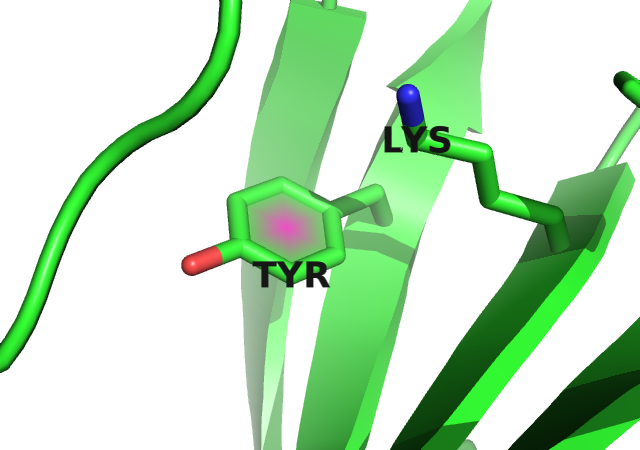
\includegraphics[width=0.5\linewidth]{img/coupling_matrix_analysis/2ayda01_37_48} \caption{Tyrosing (residue 37) and
Lysine (residue 48) forming a cation-\(\pi\) interaction in protein
2ayd.}\label{fig:coupling-matrix-pication-pymol}
\end{figure}










\begin{figure}
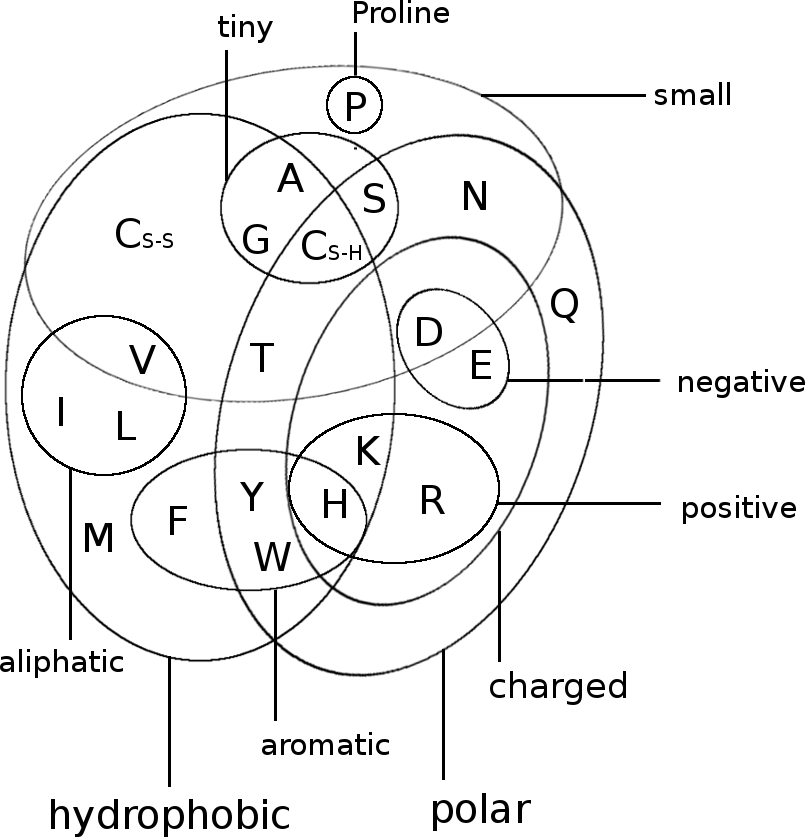
\includegraphics[width=1\linewidth]{img/amino_acid_physico_chemical_properties_venn_diagramm} \caption{Coupling Matrix for
residue pair i=37 and j=48 of PDB 2ayd chain A domain 1. Size of the
bubbles represents coupling strength and color represents the direction
of coupling: red = positive coupling, blue = negative coupling. Bars at
the x-axis represent single potentials for residue i=37 and bars at the
y-axis represent single potentials for residue j=48. Height of the bars
represents potential strength and color represents positive (red) and
negative (blue) values.}\label{fig:coupling-matrix-pication-interaction}
\end{figure}

\section{Disulfide Bonds}\label{disulfide}

Figure \ref{fig:coupling-matrix-disulfide-pymol} shows two cysteine
residues forming a covalent disulfide bond in protein 1alu. The
corresponding coupling matrix in figure
\ref{fig:coupling-matrix-disulfide-interaction} reflects the strong
interaction preference of cysteines.




\begin{figure}
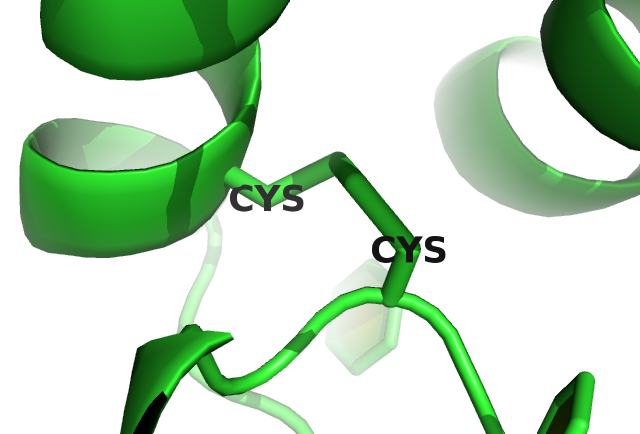
\includegraphics[width=0.5\linewidth]{img/coupling_matrix_analysis/1aluA00_54_64} \caption{Two cystein residues
(residues 54 and 64) forming a covalent disulfide bond in protein 1alu.}\label{fig:coupling-matrix-disulfide-pymol}
\end{figure}










\begin{figure}
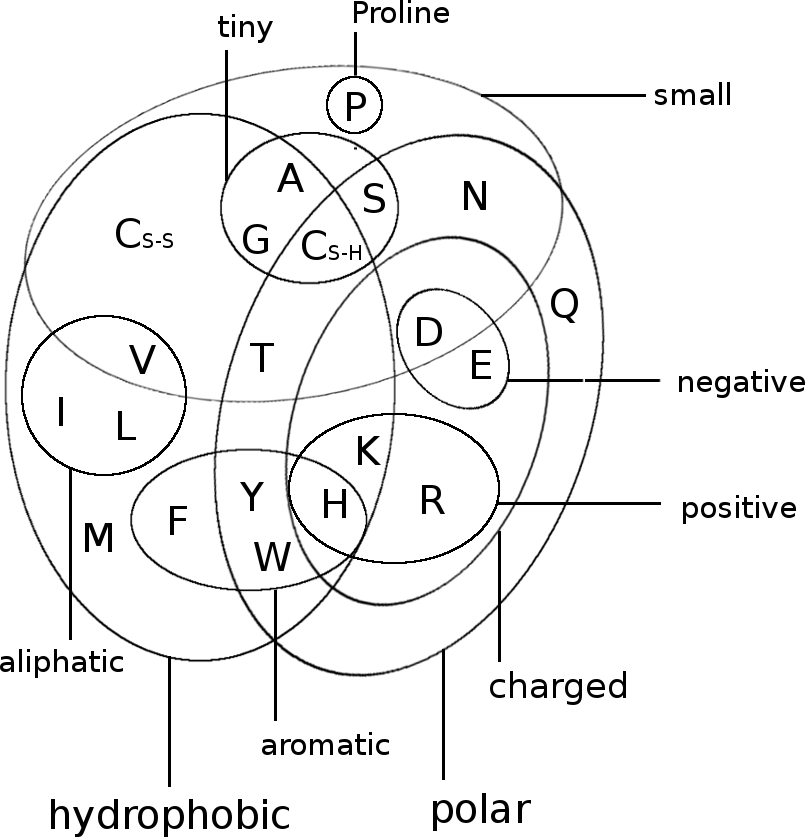
\includegraphics[width=1\linewidth]{img/amino_acid_physico_chemical_properties_venn_diagramm} \caption{Coupling Matrix for
residue pair i=54 and j=64 of PDB 1alu chain A. Size of the bubbles
represents coupling strength and color represents the direction of
coupling: red = positive coupling, blue = negative coupling. Bars at the
x-axis represent single potentials for residue i=54 and bars at the
y-axis represent single potentials for residue j=64. Height of the bars
represents potential strength and color represents positive (red) and
negative (blue) values.}\label{fig:coupling-matrix-disulfide-interaction}
\end{figure}

\section{Aromatic-Proline Interactions}\label{aromatic-proline}

Figure @ref(fig:coupling-matrix-aromatic-proline-pymol )shows a proline
and a tryptophan residue forming such a CH/\(\pi\) interaction in
protein 1aol. The corresponding coupling matrix in figure
\ref{fig:coupling-matrix-aromatic-proline} reflects this interaction
with strong positive coupling between proline and tryptophan.





\begin{figure}
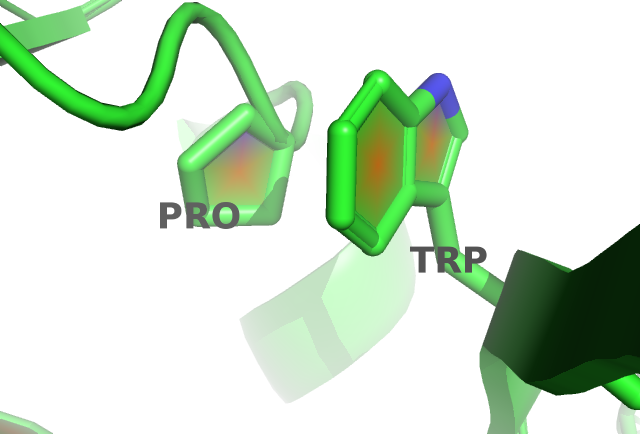
\includegraphics[width=0.5\linewidth]{img/coupling_matrix_analysis/1aolA00_17_34} \caption{Proline and
tryptophan (residues 17 and 34) stacked on top of each otherengaging in
a CH/\(\pi\) interaction in protein 1alu.}\label{fig:coupling-matrix-aromatic-proline-pymol}
\end{figure}










\begin{figure}
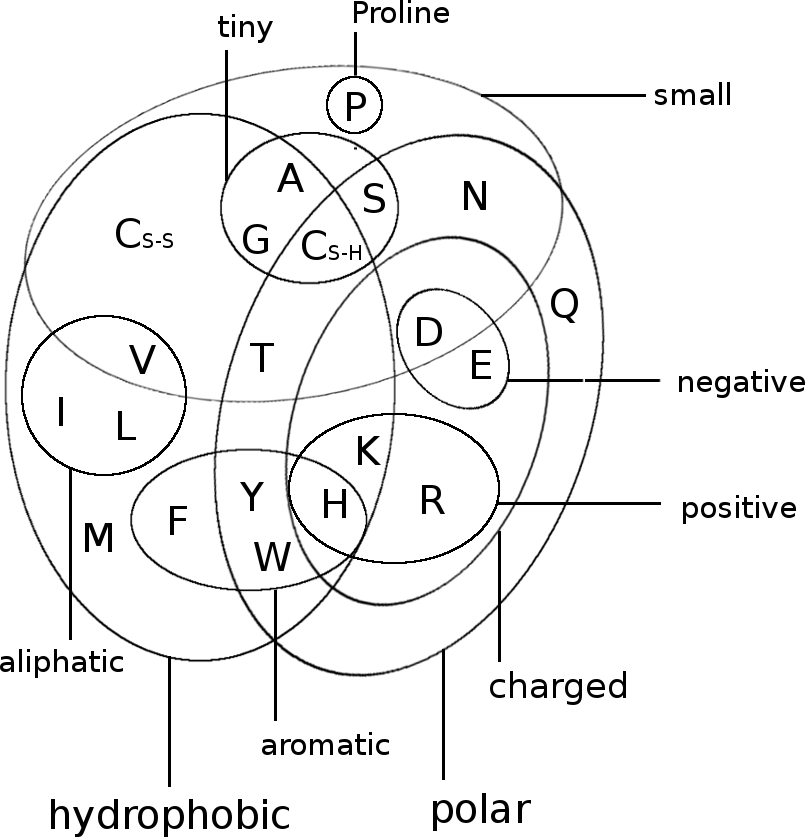
\includegraphics[width=1\linewidth]{img/amino_acid_physico_chemical_properties_venn_diagramm} \caption{Coupling Matrix for
residue pair i=17 and j=34 of PDB 1aol chain A. Size of the bubbles
represents coupling strength and color represents the direction of
coupling: red = positive coupling, blue = negative coupling. Bars at the
x-axis represent single potentials for residue i=17 and bars at the
y-axis represent single potentials for residue j=34. Height of the bars
represents potential strength and color represents positive (red) and
negative (blue) values.}\label{fig:coupling-matrix-aromatic-proline}
\end{figure}

\section{Network-like structure of aromatic
residues}\label{aromatic-network}






\begin{figure}
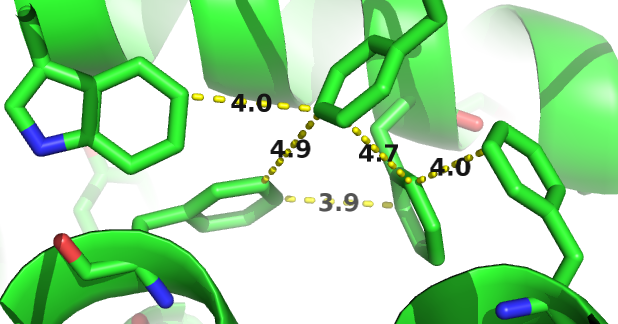
\includegraphics[width=0.5\linewidth]{img/coupling_matrix_analysis/aromatic_bundle} \caption{Network-like structure of aromatic
residues in the protein core. 80\% of aromatic residues are involved in
such networks that are important for protein stability
{[}\protect\hyperlink{ref-Burley1985}{13}{]}.}\label{fig:aromatic-network}
\end{figure}

\backmatter

\listoffigures
\addcontentsline{toc}{chapter}{List of Figures}

\listoftables
\addcontentsline{toc}{chapter}{List of Tables}

\chapter*{References}\label{references}
\addcontentsline{toc}{chapter}{References}

\hypertarget{refs}{}
\hypertarget{ref-Anfinsen1973}{}
1. Anfinsen, C.B. (1973). Principles that Govern the Folding of Protein
Chains. Science (80-. ). \emph{181}, 223--230. Available at:
\url{http://www.sciencemag.org/content/181/4096/223}.

\hypertarget{ref-Wright1999}{}
2. Wright, P.E., and Dyson, H. (1999). Intrinsically unstructured
proteins: re-assessing the protein structure-function paradigm. J. Mol.
Biol. \emph{293}, 321--331. Available at:
\href{http://www.ncbi.nlm.nih.gov/pubmed/10550212\%20http://linkinghub.elsevier.com/retrieve/pii/S0022283699931108}{http://www.ncbi.nlm.nih.gov/pubmed/10550212 http://linkinghub.elsevier.com/retrieve/pii/S0022283699931108}.

\hypertarget{ref-Samish2015}{}
3. Samish, I., Bourne, P.E., and Najmanovich, R.J. (2015). Achievements
and challenges in structural bioinformatics and computational
biophysics. Bioinformatics \emph{31}, 146--150. Available at:
\href{https://oup.silverchair-cdn.com/oup/backfile/Content\%7B/_\%7Dpublic/Journal/bioinformatics/31/1/10.1093\%7B/_\%7Dbioinformatics\%7B/_\%7Dbtu769/2/btu769.pdf?Expires=1500051331\%7B/\&\%7DSignature=WYTe4F7OxZkkcnJmsjt-r8gIyHaHX5ANqUoy6w0PUuete2b\%7B~\%7D5ZU\%7B~\%7D\%7B~\%7DD6KOB1vq5A8MgCnrq3pDHUn0OSgz0QFmtU2RYf907-}{https://oup.silverchair-cdn.com/oup/backfile/Content\{\textbackslash{}\_\}public/Journal/bioinformatics/31/1/10.1093\{\textbackslash{}\_\}bioinformatics\{\textbackslash{}\_\}btu769/2/btu769.pdf?Expires=1500051331\{\textbackslash{}\&\}Signature=WYTe4F7OxZkkcnJmsjt-r8gIyHaHX5ANqUoy6w0PUuete2b\{\textasciitilde{}\}5ZU\{\textasciitilde{}\}\{\textasciitilde{}\}D6KOB1vq5A8MgCnrq3pDHUn0OSgz0QFmtU2RYf907-}.

\hypertarget{ref-Lesk1980}{}
4. Lesk, A.M., and Chothia, C. (1980). How different amino acid
sequences determine similar protein structures: The structure and
evolutionary dynamics of the globins. J. Mol. Biol. \emph{136},
225--270. Available at:
\url{http://linkinghub.elsevier.com/retrieve/pii/0022283680903733}.

\hypertarget{ref-Sander1991}{}
5. Sander, C., and Schneider, R. (1991). Database of homology-derived
protein structures and the structural meaning of sequence alignment.
Proteins \emph{9}, 56--68. Available at:
\url{http://www.ncbi.nlm.nih.gov/pubmed/2017436}.

\hypertarget{ref-Chothia1986}{}
6. Chothia, C., and Lesk, A.M. (1986). The relation between the
divergence of sequence and structure in proteins. EMBO J. \emph{5},
823--6. Available at:
\href{http://www.ncbi.nlm.nih.gov/pubmed/3709526\%20http://www.pubmedcentral.nih.gov/articlerender.fcgi?artid=PMC1166865}{http://www.ncbi.nlm.nih.gov/pubmed/3709526 http://www.pubmedcentral.nih.gov/articlerender.fcgi?artid=PMC1166865}.

\hypertarget{ref-Marti-Renom2000}{}
7. Martí-Renom, M.A., Stuart, A.C., Fiser, A., Sánchez, R., Melo, F.,
and Šali, A. (2000). Comparative Protein Structure Modeling of Genes and
Genomes. Annu. Rev. Biophys. Biomol. Struct. \emph{29}, 291--325.
Available at:
\url{http://www.annualreviews.org/doi/10.1146/annurev.biophys.29.1.291}.

\hypertarget{ref-Dorn2014}{}
8. Dorn, M., Silva, M.B. e, Buriol, L.S., and Lamb, L.C. (2014).
Three-dimensional protein structure prediction: Methods and
computational strategies. Comput. Biol. Chem. \emph{53}, 251--276.
Available at:
\url{http://linkinghub.elsevier.com/retrieve/pii/S1476927114001248}.

\hypertarget{ref-Berman2000}{}
9. Berman, H.M. (2000). The Protein Data Bank. Nucleic Acids Res.
\emph{28}, 235--242. Available at:
\url{http://nar.oxfordjournals.org/content/28/1/235.short}.

\hypertarget{ref-Egelman2016}{}
10. Egelman, E.H. (2016). The Current Revolution in Cryo-EM. Biophysj
\emph{110}, 1008--1012. Available at:
\url{http://www.cell.com/biophysj/pdf/S0006-3495(16)00142-9.pdf}.

\hypertarget{ref-TheUniProtConsortium2013}{}
11. The UniProt Consortium (2013). Update on activities at the Universal
Protein Resource (UniProt) in 2013. Nucleic Acids Res. \emph{41},
D43--7. Available at:
\url{http://nar.oxfordjournals.org/content/41/D1/D43}.

\hypertarget{ref-Waters2002}{}
12. Waters, M.L. (2002). Aromatic interactions in model systems. Curr.
Opin. Chem. Biol. \emph{6}, 736--741. Available at:
\url{http://dx.doi.org/10.1016/S1367-5931(02)00359-9}.

\hypertarget{ref-Burley1985}{}
13. Burley, S., and Petsko, G. (1985). Aromatic-aromatic interaction: a
mechanism of protein structure stabilization. Science (80-. ).
\emph{229}, 23--28. Available at:
\url{http://www.sciencemag.org/cgi/doi/10.1126/science.3892686}.

\hypertarget{ref-Thornton1981}{}
14. Thornton, J.M. (1981). Disulphide bridges in globular proteins. J.
Mol. Biol. \emph{151}, 261--87. Available at:
\url{http://www.ncbi.nlm.nih.gov/pubmed/7338898}.

\hypertarget{ref-Bastolla2005}{}
15. Bastolla, U., and Demetrius, L. (2005). Stability constraints and
protein evolution: the role of chain length, composition and disulfide
bonds. Protein Eng. Des. Sel. \emph{18}, 405--415. Available at:
\url{https://academic.oup.com/peds/article-lookup/doi/10.1093/protein/gzi045}.

\hypertarget{ref-Donald2011}{}
16. Donald, J.E., Kulp, D.W., and DeGrado, W.F. (2011). Salt bridges:
geometrically specific, designable interactions. Proteins \emph{79},
898--915. Available at:
\href{http://www.pubmedcentral.nih.gov/articlerender.fcgi?artid=3069487\%7B/\&\%7Dtool=pmcentrez\%7B/\&\%7Drendertype=abstract}{http://www.pubmedcentral.nih.gov/articlerender.fcgi?artid=3069487\{\textbackslash{}\&\}tool=pmcentrez\{\textbackslash{}\&\}rendertype=abstract}.

\hypertarget{ref-Burley1986}{}
17. Burley, S., and Petsko, G. (1986). Amino-aromatic interactions in
proteins. FEBS Lett. \emph{203}, 139--143. Available at:
\url{http://dx.doi.org/10.1016/0014-5793(86)80730-X}.

\hypertarget{ref-Crowley2005}{}
18. Crowley, P.B., and Golovin, A. (2005). Cation-pi interactions in
protein-protein interfaces. Proteins \emph{59}, 231--9. Available at:
\url{http://www.ncbi.nlm.nih.gov/pubmed/15726638}.

\hypertarget{ref-Slutsky2004}{}
19. Slutsky, M.M., and Marsh, E.N.G. (2004). Cation-pi interactions
studied in a model coiled-coil peptide. Protein Sci. \emph{13},
2244--51. Available at:
\href{http://www.pubmedcentral.nih.gov/articlerender.fcgi?artid=2279832\%7B/\&\%7Dtool=pmcentrez\%7B/\&\%7Drendertype=abstract}{http://www.pubmedcentral.nih.gov/articlerender.fcgi?artid=2279832\{\textbackslash{}\&\}tool=pmcentrez\{\textbackslash{}\&\}rendertype=abstract}.

\hypertarget{ref-Levinthal1969}{}
20. Levinthal, C. (1969). How to Fold Graciously. 22--24. Available at:
\url{http://www.citeulike.org/user/FBerkemeier/article/380320}.

\hypertarget{ref-Rost1999}{}
21. Rost, B. (1999). Twilight zone of protein sequence alignments.
Protein Eng. Des. Sel. \emph{12}, 85--94. Available at:
\url{http://peds.oxfordjournals.org/content/12/2/85.full}.

\hypertarget{ref-Yan2013}{}
22. Yan, R., Xu, D., Yang, J., Walker, S., and Zhang, Y. (2013). A
comparative assessment and analysis of 20 representative sequence
alignment methods for protein structure prediction. Sci. Rep. \emph{3},
2619. Available at:
\url{http://www.nature.com/srep/2013/130910/srep02619/full/srep02619.html}.

\hypertarget{ref-Meier2015}{}
23. Meier, A. (2015). Automatic Prediction of Protein 3D Structures by
Probabilistic Multi-template Homology Modeling. PLoS Comput Biol
\emph{11}, 1--20.

\hypertarget{ref-Gu2009}{}
24. Gu, J., and Bourne, P.E. (2009). Structural Bioinformatics
(Wiley-Blackwell) Available at:
\url{http://www.amazon.com/Structural-Bioinformatics-Jenny-Gu/dp/0470181052}.

\hypertarget{ref-Eswar2007}{}
25. Eswar, N., Webb, B., Marti-Renom, M.A., Madhusudhan, M.S., Eramian,
D., Shen, M.-Y., Pieper, U., and Sali, A. (2007). Comparative protein
structure modeling using MODELLER. Curr. Protoc. Protein Sci.
\emph{Chapter 2}, Unit 2.9. Available at:
\url{http://www.ncbi.nlm.nih.gov/pubmed/18429317}.

\hypertarget{ref-Bates2001}{}
26. Bates, P.A., Kelley, L.A., MacCallum, R.M., and Sternberg, M.J.
(2001). Enhancement of protein modeling by human intervention in
applying the automatic programs 3D-JIGSAW and 3D-PSSM. Proteins
\emph{Suppl 5}, 39--46. Available at:
\url{http://www.ncbi.nlm.nih.gov/pubmed/11835480}.

\hypertarget{ref-Arnold2006}{}
27. Arnold, K., Bordoli, L., Kopp, J., and Schwede, T. (2006). The
SWISS-MODEL workspace: a web-based environment for protein structure
homology modelling. Bioinformatics \emph{22}, 195--201. Available at:
\url{http://bioinformatics.oxfordjournals.org/content/22/2/195.short}.

\hypertarget{ref-Gobel1994}{}
28. Göbel, U., Sander, C., Schneider, R., and Valencia, A. (1994).
Correlated mutations and residue contacts in proteins. Proteins
\emph{18}, 309--17. Available at:
\url{http://www.ncbi.nlm.nih.gov/pubmed/8208723}.

\hypertarget{ref-Dunn2008}{}
29. Dunn, S.D., Wahl, L.M., and Gloor, G.B. (2008). Mutual information
without the influence of phylogeny or entropy dramatically improves
residue contact prediction. Bioinformatics \emph{24}, 333--40. Available
at: \url{http://bioinformatics.oxfordjournals.org/content/24/3/333}.

\hypertarget{ref-Weigt2009}{}
30. Weigt, M., White, R.A., Szurmant, H., Hoch, J.A., and Hwa, T.
(2009). Identification of direct residue contacts in protein-protein
interaction by message passing. Proc. Natl. Acad. Sci. U. S. A.
\emph{106}, 67--72. Available at:
\url{http://www.pnas.org/content/106/1/67.abstract}.

\hypertarget{ref-Neher1994}{}
31. Neher, E. (1994). How frequent are correlated changes in families of
protein sequences? Proc. Natl. Acad. Sci. U. S. A. \emph{91}, 98--102.
Available at:
\href{http://www.pubmedcentral.nih.gov/articlerender.fcgi?artid=42893\%7B/\&\%7Dtool=pmcentrez\%7B/\&\%7Drendertype=abstract}{http://www.pubmedcentral.nih.gov/articlerender.fcgi?artid=42893\{\textbackslash{}\&\}tool=pmcentrez\{\textbackslash{}\&\}rendertype=abstract}.

\hypertarget{ref-Taylor1994}{}
32. Taylor, W.R., and Hatrick, K. (1994). Compensating changes in
protein multiple sequence alignments. "Protein Eng. Des. Sel. \emph{7},
341--348. Available at:
\url{http://peds.oxfordjournals.org/content/7/3/341.abstract}.

\hypertarget{ref-Oliveira2002}{}
33. Oliveira, L., Paiva, A.C.M., and Vriend, G. (2002). Correlated
mutation analyses on very large sequence families. Chembiochem \emph{3},
1010--7. Available at:
\href{http://onlinelibrary.wiley.com/doi/10.1002/1439-7633(20021004)3:10\%7B/\%\%7D3C1010::AID-CBIC1010\%7B/\%\%7D3E3.0.CO;2-T/full}{http://onlinelibrary.wiley.com/doi/10.1002/1439-7633(20021004)3:10\{\textbackslash{}\%\}3C1010::AID-CBIC1010\{\textbackslash{}\%\}3E3.0.CO;2-T/full}.

\hypertarget{ref-Clarke1995}{}
34. Clarke, N.D. (1995). Covariation of residues in the homeodomain
sequence family. Protein Sci. \emph{4}, 2269--78. Available at:
\href{http://www.pubmedcentral.nih.gov/articlerender.fcgi?artid=2143025\%7B/\&\%7Dtool=pmcentrez\%7B/\&\%7Drendertype=abstract}{http://www.pubmedcentral.nih.gov/articlerender.fcgi?artid=2143025\{\textbackslash{}\&\}tool=pmcentrez\{\textbackslash{}\&\}rendertype=abstract}.

\hypertarget{ref-Korber1993}{}
35. Korber, B. (1993). Covariation of Mutations in the V3 Loop of Human
Immunodeficiency Virus Type 1 Envelope Protein: An Information Theoretic
Analysis. Proc. Natl. Acad. Sci. \emph{90}, 7176--7180. Available at:
\href{http://www.pnas.org/content/90/15/7176.abstract?ijkey=6e1c9cbdef66bd0beefedc88ea07591b837f2213\%7B/\&\%7Dkeytype2=tf\%7B/_\%7Dipsecsha}{http://www.pnas.org/content/90/15/7176.abstract?ijkey=6e1c9cbdef66bd0beefedc88ea07591b837f2213\{\textbackslash{}\&\}keytype2=tf\{\textbackslash{}\_\}ipsecsha}.

\hypertarget{ref-Martin2005}{}
36. Martin, L.C., Gloor, G.B., Dunn, S.D., and Wahl, L.M. (2005). Using
information theory to search for co-evolving residues in proteins.
Bioinformatics \emph{21}, 4116--24. Available at:
\url{http://bioinformatics.oxfordjournals.org/content/21/22/4116.full}.

\hypertarget{ref-Atchley2000}{}
37. Atchley, W.R., Wollenberg, K.R., Fitch, W.M., Terhalle, W., and
Dress, A.W. (2000). Correlations Among Amino Acid Sites in bHLH Protein
Domains: An Information Theoretic Analysis. Mol. Biol. Evol. \emph{17},
164--178. Available at:
\href{http://mbe.oxfordjournals.org/content/17/1/164.abstract?ijkey=2a1f0a044a8fd2213955e4f2c17fa84682dd2571\%7B/\&\%7Dkeytype2=tf\%7B/_\%7Dipsecsha}{http://mbe.oxfordjournals.org/content/17/1/164.abstract?ijkey=2a1f0a044a8fd2213955e4f2c17fa84682dd2571\{\textbackslash{}\&\}keytype2=tf\{\textbackslash{}\_\}ipsecsha}.

\hypertarget{ref-Fodor2004}{}
38. Fodor, A.A., and Aldrich, R.W. (2004). Influence of conservation on
calculations of amino acid covariance in multiple sequence alignments.
Proteins \emph{56}, 211--21. Available at:
\url{http://www.ncbi.nlm.nih.gov/pubmed/15211506}.

\hypertarget{ref-Tillier2003}{}
39. Tillier, E.R., and Lui, T.W. (2003). Using multiple interdependency
to separate functional from phylogenetic correlations in protein
alignments. Bioinformatics \emph{19}, 750--755. Available at:
\href{http://bioinformatics.oxfordjournals.org/content/19/6/750.abstract?ijkey=d19c5a2492bfa46d1a02d661c29a610113da8db3\%7B/\&\%7Dkeytype2=tf\%7B/_\%7Dipsecsha}{http://bioinformatics.oxfordjournals.org/content/19/6/750.abstract?ijkey=d19c5a2492bfa46d1a02d661c29a610113da8db3\{\textbackslash{}\&\}keytype2=tf\{\textbackslash{}\_\}ipsecsha}.

\hypertarget{ref-Gouveia_Oliveira2007}{}
40. Gouveia-Oliveira, R., and Pedersen, A.G. (2007). Finding coevolving
amino acid residues using row and column weighting of mutual information
and multi-dimensional amino acid representation. Algorithms Mol. Biol.
\emph{2}, 12. Available at: \url{http://www.almob.org/content/2/1/12}.

\hypertarget{ref-Kass2002}{}
41. Kass, I., and Horovitz, A. (2002). Mapping pathways of allosteric
communication in GroEL by analysis of correlated mutations. Proteins
\emph{48}, 611--7. Available at:
\url{http://www.ncbi.nlm.nih.gov/pubmed/12211028}.

\hypertarget{ref-Noivirt2005}{}
42. Noivirt, O., Eisenstein, M., and Horovitz, A. (2005). Detection and
reduction of evolutionary noise in correlated mutation analysis. Protein
Eng. Des. Sel. \emph{18}, 247--53. Available at:
\url{http://peds.oxfordjournals.org/content/18/5/247.full}.

\hypertarget{ref-DeJuan2013}{}
43. Juan, D. de, Pazos, F., and Valencia, A. (2013). Emerging methods in
protein co-evolution. Nat. Rev. Genet. \emph{14}, 249--61. Available at:
\url{http://www.readcube.com/articles/10.1038/nrg3414?locale=en}.

\hypertarget{ref-Jones2012}{}
44. Jones, D.T., Buchan, D.W.A., Cozzetto, D., and Pontil, M. (2012).
PSICOV: precise structural contact prediction using sparse inverse
covariance estimation on large multiple sequence alignments.
Bioinformatics \emph{28}, 184--90. Available at:
\url{http://bioinformatics.oxfordjournals.org/content/28/2/184.full}.

\hypertarget{ref-Lapedes1999}{}
45. Lapedes, A., Giraud, B., Liu, L., and Stormo, G. (1999). Correlated
mutations in models of protein sequences: phylogenetic and structural
effects. \emph{33}, 236--256. Available at:
\url{http://www.citeulike.org/user/qluo/article/5092214}.

\hypertarget{ref-Burger2008}{}
46. Burger, L., and Nimwegen, E. van (2008). Accurate prediction of
protein-protein interactions from sequence alignments using a Bayesian
method. Mol. Syst. Biol. \emph{4}, 165. Available at:
\url{http://msb.embopress.org/content/4/1/165.abstract}.

\hypertarget{ref-Burger2010}{}
47. Burger, L., and Nimwegen, E. van (2010). Disentangling direct from
indirect co-evolution of residues in protein alignments. PLoS Comput.
Biol. \emph{6}, e1000633. Available at:
\url{http://dx.plos.org/10.1371/journal.pcbi.1000633}.

\hypertarget{ref-Monastyrskyy2015}{}
48. Monastyrskyy, B., D'Andrea, D., Fidelis, K., Tramontano, A., and
Kryshtafovych, A. (2015). New encouraging developments in contact
prediction: Assessment of the CASP11 results. Proteins. Available at:
\url{http://www.ncbi.nlm.nih.gov/pubmed/26474083}.

\hypertarget{ref-Jaynes1957a}{}
49. Jaynes, E.T. (1957). Information Theory and Statistical Mechanics I.
Phys. Rev. \emph{106}, 620--630. Available at:
\url{https://link.aps.org/doi/10.1103/PhysRev.106.620}.

\hypertarget{ref-Jaynes1957b}{}
50. Jaynes, E.T. (1957). Information Theory and Statistical Mechanics.
II. Phys. Rev. \emph{108}, 171--190. Available at:
\url{https://link.aps.org/doi/10.1103/PhysRev.108.171}.

\hypertarget{ref-Wainwright2007}{}
51. Wainwright, M.J., and Jordan, M.I. (2007). Graphical Models,
Exponential Families, and Variational Inference. Found. Trends Mach.
Learn. \emph{1}, 1--305. Available at:
\url{http://www.nowpublishers.com/article/Details/MAL-001}.

\hypertarget{ref-Murphy2012}{}
52. Murphy, K.P. (2012). Machine Learning: A Probabilistic Perspective
(MIT Press).

\hypertarget{ref-Morcos2011}{}
53. Morcos, F., Pagnani, A., Lunt, B., Bertolino, A., Marks, D.S.,
Sander, C., Zecchina, R., Onuchic, J.N., Hwa, T., and Weigt, M. (2011).
Direct-coupling analysis of residue coevolution captures native contacts
across many protein families. Proc. Natl. Acad. Sci. U. S. A.
\emph{108}, E1293--301. Available at:
\url{http://www.pnas.org/content/108/49/E1293.full}.

\hypertarget{ref-Marks2011}{}
54. Marks, D.S., Colwell, L.J., Sheridan, R., Hopf, T.A., Pagnani, A.,
Zecchina, R., and Sander, C. (2011). Protein 3D structure computed from
evolutionary sequence variation. PLoS One \emph{6}, e28766. Available
at: \url{http://dx.plos.org/10.1371/journal.pone.0028766}.

\hypertarget{ref-Cocco2017}{}
55. Cocco, S., Feinauer, C., Figliuzzi, M., Monasson, R., and Weigt, M.
(2017). Inverse Statistical Physics of Protein Sequences: A Key Issues
Review. arXiv. Available at: \url{https://arxiv.org/pdf/1703.01222.pdf}.

\hypertarget{ref-Koller2009}{}
56. Koller, D., and Friedman, N.I.R. (2009). Probabilistic graphical
models: Principles and Techniques (MIT Press).

\hypertarget{ref-Ekeberg2013}{}
57. Ekeberg, M., Lövkvist, C., Lan, Y., Weigt, M., and Aurell, E.
(2013). Improved contact prediction in proteins: Using pseudolikelihoods
to infer Potts models. Phys. Rev. E \emph{87}, 012707. Available at:
\url{http://link.aps.org/doi/10.1103/PhysRevE.87.012707}.

\hypertarget{ref-Stein2015a}{}
58. Stein, R.R., Marks, D.S., and Sander, C. (2015). Inferring Pairwise
Interactions from Biological Data Using Maximum-Entropy Probability
Models. PLOS Comput. Biol. \emph{11}, e1004182. Available at:
\href{http://www.pubmedcentral.nih.gov/articlerender.fcgi?artid=4520494\%7B/\&\%7Dtool=pmcentrez\%7B/\&\%7Drendertype=abstract}{http://www.pubmedcentral.nih.gov/articlerender.fcgi?artid=4520494\{\textbackslash{}\&\}tool=pmcentrez\{\textbackslash{}\&\}rendertype=abstract}.

\hypertarget{ref-Seemayer2014}{}
59. Seemayer, S., Gruber, M., and Söding, J. (2014). CCMpred-fast and
precise prediction of protein residue-residue contacts from correlated
mutations. Bioinformatics, btu500. Available at:
\url{http://bioinformatics.oxfordjournals.org/content/early/2014/08/12/bioinformatics.btu500}.

\hypertarget{ref-Ekeberg2014}{}
60. Ekeberg, M., Hartonen, T., and Aurell, E. (2014). Fast
pseudolikelihood maximization for direct-coupling analysis of protein
structure from many homologous amino-acid sequences. J. Comput. Phys.
\emph{276}, 341--356. Available at:
\url{http://www.sciencedirect.com/science/article/pii/S0021999114005178}.

\hypertarget{ref-Kamisetty2013}{}
61. Kamisetty, H., Ovchinnikov, S., and Baker, D. (2013). Assessing the
utility of coevolution-based residue-residue contact predictions in a
sequence- and structure-rich era. Proc. Natl. Acad. Sci. U. S. A.
\emph{110}, 15674--9. Available at:
\href{http://www.pubmedcentral.nih.gov/articlerender.fcgi?artid=3785744\%7B/\&\%7Dtool=pmcentrez\%7B/\&\%7Drendertype=abstract}{http://www.pubmedcentral.nih.gov/articlerender.fcgi?artid=3785744\{\textbackslash{}\&\}tool=pmcentrez\{\textbackslash{}\&\}rendertype=abstract}.

\hypertarget{ref-Balakrishnan2011}{}
62. Balakrishnan, S., Kamisetty, H., Carbonell, J.G., Lee, S.-I., and
Langmead, C.J. (2011). Learning generative models for protein fold
families. Proteins \emph{79}, 1061--78. Available at:
\url{http://www.ncbi.nlm.nih.gov/pubmed/21268112}.

\hypertarget{ref-Friedman2008}{}
63. Friedman, J., Hastie, T., and Tibshirani, R. (2008). Sparse inverse
covariance estimation with the graphical lasso. Biostatistics \emph{9},
432--41. Available at:
\url{http://biostatistics.oxfordjournals.org/content/9/3/432.abstract}.

\hypertarget{ref-Baldassi2014}{}
64. Baldassi, C., Zamparo, M., Feinauer, C., Procaccini, A., Zecchina,
R., Weigt, M., and Pagnani, A. (2014). Fast and accurate multivariate
gaussian modeling of protein families: predicting residue contacts and
protein-interaction partners. PLoS One \emph{9}, e92721. Available at:
\url{http://dx.plos.org/10.1371/journal.pone.0092721}.

\hypertarget{ref-Besag1975}{}
65. Besag, J. (1975). Statistical Analysis of Non-Lattice Data. Source
Stat. \emph{24}, 179--195. Available at:
\href{http://www.jstor.org\%20http://www.jstor.org/stable/2987782}{http://www.jstor.org http://www.jstor.org/stable/2987782}.

\hypertarget{ref-Gidas1988}{}
66. Gidas, B. (1988). Consistency of maximum likelihood and
pseudo-likelihood estimators for Gibbs Distributions. Stoch. Differ.
Syst. Stoch. Control Theory Appl. Available at:
\href{http://www.researchgate.net/publication/244456377\%7B/_\%7DConsistency\%7B/_\%7Dof\%7B/_\%7Dmaximum\%7B/_\%7Dlikelihood\%7B/_\%7Dand\%7B/_\%7Dpseudo-likelihood\%7B/_\%7Destimators\%7B/_\%7Dfor\%7B/_\%7DGibbs\%7B/_\%7DDistributions}{http://www.researchgate.net/publication/244456377\{\textbackslash{}\_\}Consistency\{\textbackslash{}\_\}of\{\textbackslash{}\_\}maximum\{\textbackslash{}\_\}likelihood\{\textbackslash{}\_\}and\{\textbackslash{}\_\}pseudo-likelihood\{\textbackslash{}\_\}estimators\{\textbackslash{}\_\}for\{\textbackslash{}\_\}Gibbs\{\textbackslash{}\_\}Distributions}.

\hypertarget{ref-Feinauer2014}{}
67. Feinauer, C., Skwark, M.J., Pagnani, A., and Aurell, E. (2014).
Improving contact prediction along three dimensions. 19. Available at:
\url{http://arxiv.org/abs/1403.0379}.

\hypertarget{ref-Zhang2016}{}
68. Zhang, H., Gao, Y., Deng, M., Wang, C., Zhu, J., Li, S.C., Zheng,
W.-M., and Bu, D. (2016). Improving residue-residue contact prediction
via low-rank and sparse decomposition of residue correlation matrix.
Biochem. Biophys. Res. Commun. Available at:
\url{http://www.sciencedirect.com/science/article/pii/S0006291X16301838}.

\hypertarget{ref-Marks2012}{}
69. Marks, D.S., Hopf, T.A., and Sander, C. (2012). Protein structure
prediction from sequence variation. Nat. Biotechnol. \emph{30},
1072--1080. Available at:
\url{http://www.nature.com/nbt/journal/v30/n11/full/nbt.2419.html}.

\hypertarget{ref-Buslje2009}{}
70. Buslje, C.M., Santos, J., Delfino, J.M., and Nielsen, M. (2009).
Correction for phylogeny, small number of observations and data
redundancy improves the identification of coevolving amino acid pairs
using mutual information. Bioinformatics \emph{25}, 1125--31. Available
at:
\href{http://www.ncbi.nlm.nih.gov/pubmed/19276150\%20http://www.pubmedcentral.nih.gov/articlerender.fcgi?artid=PMC2672635}{http://www.ncbi.nlm.nih.gov/pubmed/19276150 http://www.pubmedcentral.nih.gov/articlerender.fcgi?artid=PMC2672635}.

\hypertarget{ref-Anishchenko2017}{}
71. Anishchenko, I., Ovchinnikov, S., Kamisetty, H., and Baker, D.
(2017). Origins of coevolution between residues distant in protein 3D
structures. Proc. Natl. Acad. Sci., 201702664. Available at:
\href{http://www.ncbi.nlm.nih.gov/pubmed/28784799\%20http://www.pnas.org/lookup/doi/10.1073/pnas.1702664114}{http://www.ncbi.nlm.nih.gov/pubmed/28784799 http://www.pnas.org/lookup/doi/10.1073/pnas.1702664114}.

\hypertarget{ref-Finn2016}{}
72. Finn, R.D., Coggill, P., Eberhardt, R.Y., Eddy, S.R., Mistry, J.,
Mitchell, A.L., Potter, S.C., Punta, M., Qureshi, M., and
Sangrador-Vegas, A. \emph{et al.} (2016). The Pfam protein families
database: towards a more sustainable future. Nucleic Acids Res.
\emph{44}, D279--D285. Available at:
\url{https://academic.oup.com/nar/article-lookup/doi/10.1093/nar/gkv1344}.

\hypertarget{ref-Remmert2012}{}
73. Remmert, M., Biegert, A., Hauser, A., and Söding, J. (2012).
HHblits: lightning-fast iterative protein sequence searching by HMM-HMM
alignment. Nat. Methods \emph{9}, 173--5. Available at:
\url{http://dx.doi.org/10.1038/nmeth.1818}.

\hypertarget{ref-Espada2014}{}
74. Espada, R., Parra, R.G., Mora, T., Walczak, A.M., and Ferreiro, D.
(2015). Capturing coevolutionary signals in repeat proteins. BMC
Bioinformatics \emph{16}, 207. Available at:
\url{http://arxiv.org/abs/1407.6903}.

\hypertarget{ref-Toth-Petroczy2016}{}
75. Toth-Petroczy, A., Palmedo, P., Ingraham, J., Hopf, T.A., Berger,
B., Sander, C., Marks, D.S., Alexander, P., He, Y., and Chen, Y.
\emph{et al.} (2016). Structured States of Disordered Proteins from
Genomic Sequences. Cell \emph{167}, 158--170.e12. Available at:
\url{http://linkinghub.elsevier.com/retrieve/pii/S0092867416312430}.

\hypertarget{ref-Hopf2012}{}
76. Hopf, T.A., Colwell, L.J., Sheridan, R., Rost, B., Sander, C., and
Marks, D.S. (2012). Three-dimensional structures of membrane proteins
from genomic sequencing. Cell \emph{149}, 1607--21. Available at:
\href{http://www.pubmedcentral.nih.gov/articlerender.fcgi?artid=3641781\%7B/\&\%7Dtool=pmcentrez\%7B/\&\%7Drendertype=abstract}{http://www.pubmedcentral.nih.gov/articlerender.fcgi?artid=3641781\{\textbackslash{}\&\}tool=pmcentrez\{\textbackslash{}\&\}rendertype=abstract}.

\hypertarget{ref-Bettsa}{}
77. Betts, M.J., and Russell, R.B. Amino Acid Properties and
Consequences of Substitutions. In Bioinforma. genet. (Chichester, UK:
John Wiley \& Sons, Ltd), pp. 289--316. Available at:
\url{http://doi.wiley.com/10.1002/0470867302.ch14}.

\hypertarget{ref-Duarte2010}{}
78. Duarte, J.M., Sathyapriya, R., Stehr, H., Filippis, I., and Lappe,
M. (2010). Optimal contact definition for reconstruction of contact
maps. BMC Bioinformatics \emph{11}, 283. Available at:
\url{http://www.biomedcentral.com/1471-2105/11/283}.

\hypertarget{ref-Lee2009}{}
79. Lee, B.-C., and Kim, D. (2009). A new method for revealing
correlated mutations under the structural and functional constraints in
proteins. Bioinformatics \emph{25}, 2506--13. Available at:
\url{http://www.ncbi.nlm.nih.gov/pubmed/19628501}.

\hypertarget{ref-Wang2015}{}
80. Wang, Y., and Barth, P. (2015). Evolutionary-guided de novo
structure prediction of self-associated transmembrane helical proteins
with near-atomic accuracy. Nat. Commun. \emph{6}, 7196. Available at:
\url{http://www.nature.com/ncomms/2015/150521/ncomms8196/abs/ncomms8196.html}.

\hypertarget{ref-Sutto2015}{}
81. Sutto, L., Marsili, S., Valencia, A., and Gervasio, F.L. (2015).
From residue coevolution to protein conformational ensembles and
functional dynamics. Proc. Natl. Acad. Sci. U. S. A., 1508584112.
Available at:
\url{http://www.pnas.org/content/early/2015/10/20/1508584112.abstract}.

\hypertarget{ref-Jana2014}{}
82. Jana, B., Morcos, F., and Onuchic, J.N. (2014). From structure to
function: the convergence of structure based models and co-evolutionary
information. Phys. Chem. Chem. Phys. \emph{16}, 6496. Available at:
\href{http://www.ncbi.nlm.nih.gov/pubmed/24603809\%20http://xlink.rsc.org/?DOI=c3cp55275f}{http://www.ncbi.nlm.nih.gov/pubmed/24603809 http://xlink.rsc.org/?DOI=c3cp55275f}.

\hypertarget{ref-DosSantos2015a}{}
83. Dos Santos, R.N., Morcos, F., Jana, B., Andricopulo, A.D., and
Onuchic, J.N. (2015). Dimeric interactions and complex formation using
direct coevolutionary couplings. Sci. Rep. \emph{5}, 13652. Available
at:
\url{http://www.nature.com/srep/2015/150904/srep13652/full/srep13652.html}.

\hypertarget{ref-Ovchinnikov2015b}{}
84. Ovchinnikov, S., Kim, D.E., Wang, R.Y.-R., Liu, Y., DiMaio, F., and
Baker, D. (2015). Improved de novo structure prediction in CASP11 by
incorporating Co-evolution information into rosetta. Proteins. Available
at: \url{http://www.ncbi.nlm.nih.gov/pubmed/26677056}.

\hypertarget{ref-Noel2016}{}
85. Noel, J.K., Morcos, F., and Onuchic, J.N. (2016). Sequence
co-evolutionary information is a natural partner to minimally-frustrated
models of biomolecular dynamics. F1000Research \emph{5}. Available at:
\url{http://f1000research.com/articles/5-106/v1}.

\hypertarget{ref-Sfriso2016}{}
86. Sfriso, P., Duran-Frigola, M., Mosca, R., Emperador, A., Aloy, P.,
and Orozco, M. (2016). Residues Coevolution Guides the Systematic
Identification of Alternative Functional Conformations in Proteins.
Structure \emph{24}, 116--126. Available at:
\url{http://linkinghub.elsevier.com/retrieve/pii/S0969212615004657}.

\hypertarget{ref-Coucke2016}{}
87. Coucke, A., Uguzzoni, G., Oteri, F., Cocco, S., Monasson, R., and
Weigt, M. (2016). Direct coevolutionary couplings reflect biophysical
residue interactions in proteins. J. Chem. Phys. \emph{145}, 174102.
Available at:
\url{http://scitation.aip.org/content/aip/journal/jcp/145/17/10.1063/1.4966156}.

\hypertarget{ref-Aurell2012}{}
88. Aurell, E., and Ekeberg, M. (2012). Inverse Ising Inference Using
All the Data. Phys. Rev. Lett. \emph{108}, 090201. Available at:
\url{https://link.aps.org/doi/10.1103/PhysRevLett.108.090201}.

\hypertarget{ref-Jones2015a}{}
89. Jones, D.T., Singh, T., Kosciolek, T., and Tetchner, S. (2015).
MetaPSICOV: combining coevolution methods for accurate prediction of
contacts and long range hydrogen bonding in proteins. Bioinformatics
\emph{31}, 999--1006. Available at:
\url{http://bioinformatics.oxfordjournals.org/content/31/7/999.short}.

\hypertarget{ref-Ma2015a}{}
90. Ma, J., Wang, S., Wang, Z., and Xu, J. (2015). Protein contact
prediction by integrating joint evolutionary coupling analysis and
supervised learning. Bioinformatics, btv472. Available at:
\url{http://bioinformatics.oxfordjournals.org/content/early/2015/09/04/bioinformatics.btv472}.

\hypertarget{ref-Miyazawa1999a}{}
91. Miyazawa, S., and Jernigan, R.L. (1999). Self-consistent estimation
of inter-residue protein contact energies based on an equilibrium
mixture approximation of residues. Proteins \emph{34}, 49--68. Available
at: \url{http://www.ncbi.nlm.nih.gov/pubmed/10336383}.

\hypertarget{ref-Sillitoe2015}{}
92. Sillitoe, I., Lewis, T.E., Cuff, A., Das, S., Ashford, P., Dawson,
N.L., Furnham, N., Laskowski, R.A., Lee, D., and Lees, J.G. \emph{et
al.} (2015). CATH: comprehensive structural and functional annotations
for genome sequences. Nucleic Acids Res. \emph{43}, D376--D381.
Available at:
\url{https://academic.oup.com/nar/article-lookup/doi/10.1093/nar/gku947}.

\hypertarget{ref-Kingma2014}{}
93. Kingma, D., and Ba, J. (2014). Adam: A Method for Stochastic
Optimization. Available at: \url{http://arxiv.org/abs/1412.6980}.

\hypertarget{ref-Atchley2005}{}
94. Atchley, W.R., Zhao, J., Fernandes, A.D., and Drüke, T. (2005).
Solving the protein sequence metric problem. Proc. Natl. Acad. Sci. U.
S. A. \emph{102}, 6395--400. Available at:
\url{http://www.pnas.org/content/102/18/6395.abstract}.

\hypertarget{ref-Li2011}{}
95. Li, Y., Fang, Y., and Fang, J. (2011). Predicting residue-residue
contacts using random forest models. Bioinformatics \emph{27}, 3379--84.
Available at:
\url{http://bioinformatics.oxfordjournals.org/content/27/24/3379.long}.

\hypertarget{ref-Zhu1999}{}
96. Zhu, H., and Braun, W. (1999). Sequence specificity, statistical
potentials, and three-dimensional structure prediction with
self-correcting distance geometry calculations of beta-sheet formation
in proteins. Protein Sci. \emph{8}, 326--42. Available at:
\href{http://www.pubmedcentral.nih.gov/articlerender.fcgi?artid=2144259\%7B/\&\%7Dtool=pmcentrez\%7B/\&\%7Drendertype=abstract}{http://www.pubmedcentral.nih.gov/articlerender.fcgi?artid=2144259\{\textbackslash{}\&\}tool=pmcentrez\{\textbackslash{}\&\}rendertype=abstract}.

\hypertarget{ref-Fodor2004a}{}
97. Fodor, A.A., and Aldrich, R.W. (2004). Influence of conservation on
calculations of amino acid covariance in multiple sequence alignments.
Proteins \emph{56}, 211--21. Available at:
\url{http://www.ncbi.nlm.nih.gov/pubmed/15211506}.


\end{document}
